\documentclass[fr]{../../../eplexercises}

\RequirePackage{titlesec}
\titleformat
{\section} % command
[hang] % shape
{\bfseries\Large} % format
{\thesection} % label
{0.5ex} % sep
{} % before-code

\usepackage{../fitch}
\usepackage{pdfpages}

\usepackage{../../../eplcode}
\definecolor{mygray}{rgb}{0.5,0.5,0.5} % needed by: 14, 17
\lstset{language=Prolog, frame = single, numbers=left, numbersep=-0.5cm, numberstyle=\small\color{mygray}, escapeinside={\%*}{*)}}

\newcommand{\true}{\mathrm{true}}
\newcommand{\false}{\mathrm{false}}
\newcommand{\val}{\mathrm{val}}
\newcommand{\VAL}{\mathrm{VAL}}
\newcommand{\decale}{\par\nodecale\hspace*{20pt}\ignorespaces}

\hypertitle{logique-INGI1101}{5}{INGI}{1101}
{Maxime Dimidschstein\and Basile Cassiers\and Nicolas Vanvyve\and Adrien Ballet\and Samuel Monroe\and Sébastien Mottet\and Grâce Musuvaho\and  Mathias Novak\and Céline Deknop}
{Peter Van Roy}

% OR
\pgfkeys{
	orGate/.is family,
	orGate,
	x/.initial=0,
	y/.initial=0,
	l/.initial=or,
}
\newcommand\orGateSet[1]{\pgfkeys{orGate, #1}}
\newcommand\orGate[1][]{
	\orGateSet{#1,
    x/.get=\x,
    y/.get=\y,
		l/.get=\l,
  }
	\draw (\x, 1 + \y) to [out=0,in=120] (0.85 + \x, 0.5 + \y);
	\draw (\x, \y) to [out=0,in=250] (0.85 + \x, 0.5 + \y);
	\draw (\x, \y) to [out=60,in=270] (0.2 + \x, 0.5 + \y);
	\draw (\x, 1 + \y) to [out=300,in=90] (0.2 + \x, 0.5 + \y);
	\draw (\x, 0.2 + \y) -- (0.12 + \x, 0.2 + \y);
	\draw (\x, 0.8 + \y) -- (0.12 + \x, 0.8 + \y);
	\draw (0.85 + \x, 0.5 + \y) -- (1 + \x, 0.5 + \y);
	\node at (\x + 0.5, \y + 0.5) {\tiny \textsf{\l}};
}

% NOR
\pgfkeys{
	norGate/.is family,
	norGate,
	x/.initial=0,
	y/.initial=0,
	l/.initial=nor,
}
\newcommand\norGateSet[1]{\pgfkeys{norGate, #1}}
\newcommand\norGate[1][]{
	\norGateSet{#1,
    x/.get=\x,
    y/.get=\y,
		l/.get=\l,
  }
	\draw (\x, 1 + \y) to [out=0,in=120] (0.85 + \x, 0.5 + \y);
	\draw (\x, \y) to [out=0,in=250] (0.85 + \x, 0.5 + \y);
	\draw (\x, \y) to [out=60,in=270] (0.2 + \x, 0.5 + \y);
	\draw (\x, 1 + \y) to [out=300,in=90] (0.2 + \x, 0.5 + \y);
	\draw (\x, 0.2 + \y) -- (0.12 + \x, 0.2 + \y);
	\draw (\x, 0.8 + \y) -- (0.12 + \x, 0.8 + \y);
	\draw (0.85 + \x, 0.5 + \y) -- (1 + \x, 0.5 + \y);
	\draw[fill = white] (0.85 + \x, 0.5 + \y) circle (0.04);
	\node at (\x + 0.5, \y + 0.5) {\tiny \textsf{\l}};
}

% AND
\pgfkeys{
	andGate/.is family,
	andGate,
	x/.initial=0,
	y/.initial=0,
	l/.initial=and,
}
\newcommand\andGateSet[1]{\pgfkeys{andGate, #1}}
\newcommand\andGate[1][]{
	\andGateSet{#1,
    x/.get=\x,
    y/.get=\y,
		l/.get=\l,
  }
	\draw (0.1 + \x, \y) -- (0.1 + \x, 1 + \y);
	\draw (0.1 + \x, \y) -- (0.6 + \x, \y);
	\draw (0.1 + \x, 1 + \y) -- (0.6 + \x, 1 + \y);
	\draw (0.6 + \x, \y) to [out=0, in=270] (0.9 + \x, 0.5 + \y);
	\draw (0.6 + \x, 1 + \y) to [out=0, in=90] (0.9 + \x, 0.5 + \y);
	\draw (\x, 0.2 + \y) -- (0.1 + \x, 0.2 + \y);
	\draw (\x, 0.8 + \y) -- (0.1 + \x, 0.8 + \y);
	\draw (0.9 + \x, 0.5 + \y) -- (1 + \x, 0.5 + \y);
	\node at (\x + 0.5, \y + 0.5) {\tiny \textsf{\l}};
}

% NAND
\pgfkeys{
	nandGate/.is family,
	nandGate,
	x/.initial=0,
	y/.initial=0,
	l/.initial=nand,
}
\newcommand\nandGateSet[1]{\pgfkeys{nandGate, #1}}
\newcommand\nandGate[1][]{
	\nandGateSet{#1,
    x/.get=\x,
    y/.get=\y,
		l/.get=\l,
  }
	\draw (0.1 + \x, \y) -- (0.1 + \x, 1 + \y);
	\draw (0.1 + \x, \y) -- (0.6 + \x, \y);
	\draw (0.1 + \x, 1 + \y) -- (0.6 + \x, 1 + \y);
	\draw (0.6 + \x, \y) to [out=0, in=270] (0.9 + \x, 0.5 + \y);
	\draw (0.6 + \x, 1 + \y) to [out=0, in=90] (0.9 + \x, 0.5 + \y);
	\draw (\x, 0.2 + \y) -- (0.1 + \x, 0.2 + \y);
	\draw (\x, 0.8 + \y) -- (0.1 + \x, 0.8 + \y);
	\draw (0.9 + \x, 0.5 + \y) -- (1 + \x, 0.5 + \y);
	\draw[fill = white] (0.9 + \x, 0.5 + \y) circle (0.04);
	\node at (\x + 0.5, \y + 0.5) {\tiny \textsf{\l}};
}

% NOT
\pgfkeys{
	notGate/.is family,
	notGate,
	x/.initial=0,
	y/.initial=0,
	l/.initial=not,
}
\newcommand\notGateSet[1]{\pgfkeys{notGate, #1}}
\newcommand\notGate[1][]{
	\notGateSet{#1,
    x/.get=\x,
    y/.get=\y,
		l/.get=\l,
  }
	\draw (0.1 + \x, \y) -- (0.1 + \x, 1 + \y);
	\draw (0.1 + \x, \y) -- (0.9 + \x, 0.5 + \y);
	\draw (0.1 + \x, 1 + \y) -- (0.9 + \x, 0.5 + \y);
	\draw (\x, 0.5 + \y) -- (0.1 + \x, 0.5 + \y);
	\draw (0.9 + \x, 0.5 + \y) -- (1 + \x, 0.5 + \y);
	\draw[fill = white] (0.9 + \x, 0.5 + \y) circle (0.04);
	\node at (\x + 0.4, \y + 0.5) {\tiny \textsf{\l}};
}

% T
\pgfkeys{
	tWire/.is family,
	tWire,
	x/.initial=0,
	y/.initial=0,
}
\newcommand\tWireSet[1]{\pgfkeys{tWire, #1}}
\newcommand\tWire[1][]{
	\notGateSet{#1,
    x/.get=\x,
    y/.get=\y,
  }
	\draw (\x, 0.5 + \y) -- (\x + 1, 0.5 + \y);
	\draw (\x + 0.5, 0.5 + \y) -- (\x + 0.5 , \y);
}

\pgfkeys{
  mygrid/.is family,
  mygrid,
  min x/.initial=-5,
  max x/.initial=5,
  min y/.initial=-5,
  max y/.initial=5,
  small step/.initial=.1,
  step/.initial=1,
  big step/.initial=5,
  color/.initial=red,
}
\newcommand\mygridset[1]{\pgfkeys{mygrid,#1}}
\newcommand\mygrid[1][]{
  \mygridset{#1,
    min x/.get=\gridminx,
    max x/.get=\gridmaxx,
    min y/.get=\gridminy,
    max y/.get=\gridmaxy,
    small step/.get=\gridsmallstep,
    step/.get=\gridstep,
    big step/.get=\gridbigstep,
    color/.get=\gridcolor
  }

  \draw [step=\gridsmallstep, help lines,\gridcolor!20]
  (\gridminx,\gridminy) grid (\gridmaxx,\gridmaxy);
  \draw [step=\gridstep, help lines,\gridcolor!40]
  (\gridminx,\gridminy) grid (\gridmaxx,\gridmaxy);
  \draw [step=\gridbigstep, help lines,\gridcolor!100]
  (\gridminx,\gridminy) grid (\gridmaxx,\gridmaxy);
  \foreach \x in {\gridminx,...,\gridmaxx} {
    \node[below,font=\tiny] at (\x,\gridminy) {$\x$};
    \node[above,font=\tiny] at (\x,\gridmaxy) {$\x$};
  };
  \foreach \y in {\gridminy,...,\gridmaxy} {
    \node[left,font=\tiny] at (\gridminx,\y) {$\y$};
    \node[right,font=\tiny] at (\gridmaxx,\y) {$\y$};
  };
}

\newcommand\loeq{\Lleftarrow\!\!\!\!\Rrightarrow }

\newcommand\enter[0]{
	{\color{white} newline}
}

\newif\ifanswers
\answerstrue

\newenvironment{sol}
{
\textbf{Solution} \\
}
{
\vspace{0.25cm}
}
\renewcommand\t[1]{\text{#1}}


\section*{Avant propos}
Ce document reprend les solutions des exercices du cours LINGI1101 dispensé par M. Peter Van Roy au cours de l'année académique 2016-2017.\\
La quasi totalité de ces solutions ont été rédigées par des étudiants\footnote{La solution du TP 3 a été publieé par erreur par un assistant}, et il est donc important de rester critique en les consultant : des erreurs subsistent, et la matière peut avoir changé.

Une partie du document a été révisée par un assistant, François Aubry

N'hésitez pas à vous servir de ce document et à le reprendre pour le corriger, l'améliorer et l'étendre.
A ce jour, certain exercices sont encore sans solution ou incomplets, en voici une liste non exhaustive:
\begin{itemize}
	\item TP 4 ex. 3
	\item TP 7 ex. 5, 7, 8.1
	\item TP 8 ex. 5.1, 5.2
	\item TP 10 ex. 9
\end{itemize}

\paragraph{\large{N.B. :}} Bien que les TP portent en grande partie sur les preuves, l'examen est lui beaucoup plus théorique et porte sur des exemples vu au cours.
%\section*{TEMPLATE}
Le syllabus peut être trouvé à l'adresse \url{https://github.com/petervanroy/lingi1101}.
C'est de là que proviennent la majorité des templates utilisés dans ce solutionnaire, inspirez-vous en.\\
Lorsque vous trouvez une nouvelle structure qui n'a pas encore été employée dans ce rapport, tapez-en un exemple ici dans une section, en plus de la mettre dans votre partie.
(Et faites en sorte que ça compile!)
Comme ça les prochains pourront également s'en servir sans devoir fouiller partout.\\
Cette partie ne sera pas inclue dans le rapport final, elle sert uniquement lors de sa rédaction.

\subsection*{Quantificateurs et symboles}
\begin{itemize}
    \item \textbf{Et logique} : $\land$
    \item \textbf{Ou logique} : $\lor$
    \item \textbf{Négation} : $\neg$
    \item \textbf{Pour tout} : $\forall$
    \item \textbf{Il existe} : $\exists$
    \item \textbf{Implication} : $\Rightarrow$
    \item \textbf{Si et seulement si} : $\Leftrightarrow$
    \item \textbf{Tautologie} : $\models$
    \item \textbf{Conséquence logique} : $\Rrightarrow$
    \item \textbf{Équivalence logique} : $\Lleftarrow \Rrightarrow$
\end{itemize}


\subsection*{Règle - cas - résultat}
\begin{enumerate}
  \item Règle: $\forall$ $x$, $sac(x)$ $\Rightarrow$ $blanc(x)$
  \item Cas: $sac(a)$, $sac(b)$, $\cdots$\\
  \rule{5.5cm}{.1pt} 
  \item Résultat: $blanc(a)$, $blanc(b)$, $\cdots$
\end{enumerate}

\subsection*{Table de vérité}
\begin{center}
	\begin{tabular}{cc|ccccc}
		$P$ & $Q$ & $\lnot P$ & $\lnot Q$ & $\lnot( P \land Q)$ & $P \land Q$ & $ (\lnot P \lor \lnot Q)$\\
		\hline
		F&F&T&T&T&F&T\\
		T&F&F&T&T&F&T\\
		F&T&T&F&T&F&T\\
		T&T&F&F&F&T&F\\
	\end{tabular}
\end{center}

\subsection*{Règle BNF}
\begin{tabular}{rrl}
  $\textrm{<identificateur>}$ & ::= & $A$ | $B$ | $C$ | $D$ | \dots \\
  $\textrm{<proposition>}$
  & ::= & $\true$ \\
  & | & $\false$ \\
  & | & $\textrm{<identificateur>}$ \\
  & | & $(\textrm{<proposition>})$ \\
  & | & $\lnot \textrm{<proposition>}$ \\
  & | & $\textrm{<proposition>} \land \textrm{<proposition>}$ \\
  & | & $\textrm{<proposition>} \lor \textrm{<proposition>}$ \\
  & | & $\textrm{<proposition>} \Rightarrow \textrm{<proposition>}$ \\
  & | & $\textrm{<proposition>} \Leftrightarrow \textrm{<proposition>}$
\end{tabular}

%\subsection*{Pseudocode}

%\begin{algorithm}[H]
%\While{$false \not\in S$ et $\exists$? clauses résolvables non résolues}{
%	\begin{itemize}
%		\item choisir $C_1,C_2 \in S$ tel que $\exists P \in C_1, \lnot P \in C_2$ 		
%		\item calculer r:=$C_1 - \{P\} \lor C_2 - \{\lnot P\}$
%		\item calculer S:= $S \cup \{r\}$
%	\end{itemize}
%}
%\eIf{$false \in S$}{C est prouvé}{C n'est pas prouvé}
%\end{algorithm}

\subsubsection*{Exemple de résolution}
\begin{tabbing}
\hspace{3cm}\=\hspace{2cm}\=\kill
C$_{1}$ : P $\lor$ Q \\
C$_{2}$ : P $\lor$ R \\
C$_{3}$ : $\lnot$Q $\lor$ $\lnot$R \\
C : P \> \> \{C$_{1}$,C$_{2}$,C$_{3}$,$\lnot$C\}
\end{tabbing}

\noindent \emph{Quelques pas de résolution :}

\noindent C$_{1}$ + $\lnot$C $\rightarrow$  Q (C$_{5}$) \newline
C$_{2}$ + $\lnot$C $\rightarrow$ R  (C$_{6}$) \newline
C$_{3}$ + C$_{5}$ $\rightarrow$ $\lnot$R (C$_{7}$) \newline 
C$_{6}$ + C$_{7}$ $\rightarrow$ \underline{false} ($\in$ S donc C est prouvé) \newline


\subsubsection*{Preuve}

\begin{tabular}{|l|l|}
\hline
1. A$\Rightarrow$B & prémisse \\
2. C$\Rightarrow$D & prémisse \\
3. B$\lor$D $\Rightarrow$E & prémisse \\
4. $\lnot$E & prémisse \\ 
\indent 5. A & hypothèse \\
\indent 6. B & modus ponens (1) \\
\indent 7. B$\lor$D & addition (6) \\
\indent 8. E & modus ponens (7) \\
9. $\lnot$A & preuve indirecte \\
\indent 10. C & hypothèse \\
\indent 11. D & modus ponens (2) \\
\indent 12. D$\lor$B & addition (11) \\
\indent 13. B$\lor$D & commutativité (12)\\
\indent 14. E & modus ponens (9) \\
15. $\lnot$C & preuve indirecte \\
16. $\lnot$A $\land$ $\lnot$C & conjonction (9,15) \\
\hline
\end{tabular}\\

\subsection*{Tracer des graphes avec Tikz}

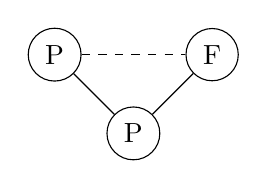
\begin{tikzpicture}
\coordinate (A) at (0,1);
\coordinate (B) at (1,0);
\coordinate (C) at (2,1);


\node[draw,circle] (A) at (A){P};
\node[draw,circle] (B) at (B){P};
\node[draw] (C) at (C){F};

\draw  (A)--(B);
\draw [dashed] (A)--(C);
\draw (C)--(B);

\end{tikzpicture}



\section{TP 1}
%\addcontentsline{toc}{section}{TP 1}


% \subsection*{Rappel}

% Sémantique des connecteurs logiques:

% \begin{center}
% \begin{tabular}{ c c | c c c c c c }
% $p$ & $q$ & $\neg p$ & $p \land q$ & $p \lor q$ & $p \Rightarrow q$ & $p \Leftrightarrow q$ & $p \oplus q$ \\
% \hline
%  T  &  T  & F        & T            & T          & T                 & T                     & F            \\
%  T  &  F  & F        & F            & T          & F                 & F                     & T            \\
%  F  &  T  & T        & F            & T          & T                 & F                     & T            \\
%  F  &  F  & T        & F            & F          & T                 & T                     & F
% \end{tabular}
% \end{center}

% % Portes logiques (ici on considère que des portes a deux inputs):
% %
% % \begin{center}
% % \begin{tikzpicture}
% % %\mygrid[min x=-5, max x=5,min y=-5,max y=5,color=blue]
% % \notGate[x=0,y=0]
% % \andGate[x=2,y=0]
% % \nandGate[x=4,y=0]
% % \orGate[x=6,y=0]
% % \norGate[x=8,y=0]
% % \end{tikzpicture}
% % \end{center}

% Convention de précédances des connecteur logiques:

% \begin{center}
% \begin{tabular}{c c c c c}
% $\neg$ & $\land$ & $\lor$ & $\Rightarrow$ & $\Leftrightarrow$
% \end{tabular}
% \end{center}

% \newpage

% \section*{TP 1}

\subsection*{Exercice 1}
Expliquez ce qu'est une interprétation et un modèle en logique propositionnelle.


\subsubsection*{Solution}
    \begin{itemize}
            \item L'\textbf{interprétation} est une fonction :
            \begin{equation*}
                val_{I}(Ep)\rightarrow \left \{true, false \right \}
            \end{equation*}

            \item Un \textbf{modèle} est une interprétation telle que

            \begin{equation*}
                VAL_{I}(p) = True
            \end{equation*}

        \end{itemize}

% \subsection*{Exercice }
% Pour chaque phrase, identifiez les connecteurs logiques et les propositions.
% \begin{enumerate}
% 	\item \textit{Je vais à la piscine ou je vais au cinéma.}
% 	\item \textit{Je vais soit à la piscine soit au cinéma.}
% \end{enumerate}
%

\subsection*{Exercice 2}
Si je vous dis: \textit{s'il fait beau alors je vais faire du vélo}, dans quelles situations je suis un menteur?

\begin{center}
\begin{tabular}{l l | l}
& & Menteur? \\
\hline
\multicolumn{1}{ l| }{Il a fait beau} & J'ai fait du vélo &  \\
\multicolumn{1}{ l| }{Il a fait beau} & Je n'ai pas fait du vélo & \\
\multicolumn{1}{ l| }{Il n'as pas fait beau} & J'ai fait du vélo & \\
\multicolumn{1}{ l| }{Il n'as pas fait beau} & Je n'ai pas fait du vélo &
\end{tabular}
\end{center}

Comparez ceci avec la table de vérité de $P \Rightarrow Q$:

\begin{center}
\begin{tabular}{c c | c}
$P$ & $Q$ & $P \Rightarrow Q$ \\
\hline
 T & T & T \\
 T & F & F \\
 F & T & T \\
 F & F & T
\end{tabular}
\end{center}



\subsubsection*{Solution}

    Posons tout d'abord les propositions suivantes :
    \begin{itemize}
        \item A : Il a fait beau
        \item B : J'ai fait du vélo
        \item M : Je suis un menteur
    \end{itemize}


    \begin{center}
    	\begin{tabular}{cc|c}
    		A & B & M\\
    		\hline
    		T & T & F\\
    		T & F & T\\
    		F & T & F\\
    		F & F & F\\
    	\end{tabular}
    \end{center}


% \subsection*{Exercice }
% Considérons les propositions suivantes:
% \begin{align*}
% P & = \textit{le voleur est jeune} & Q & = \textit{le voleur est pendu} \\
% R & = \textit{le voleur va vieillir} & S & = \textit{le voleur va voler}
% \end{align*}
% Écrivez en Français les formules suivantes:
% $$
% P \land Q \Rightarrow \neg R \land \neg S \quad \text{et} \quad P \land Q \Rightarrow \neg (R \lor S)
% $$
% Quelle est la différence entre les deux?
%

% \subsection*{Exercice }
% A l'entrée d'un bar, une affiche dit: \\
%
% \textit{Si le portier juge que vous avez plus de 18 ans alors il vous laisse renter.} \\
%
% Que peut-on conclure si quelqu'un de moins de 18 ans se présente?
%

% \subsection*{Exercice }
% L'affirmation suivante est-elle vrai ou fausse? \\
%
% \textit{Si un cheval possède des ailes alors il sait chanter.}
%

% \subsection*{Exercice }
% Dans un restaurant, votre père a demandé du poisson, votre mère un plat végetarien
% et vous de la viande. Après un certain temps le serveur arrive et demande
% ``Qui a demandé du poisson?'' et donne l'assiette à votre père. Il demande alors
% ``Qui a demandé de la viande?'' et vous donne l'assiette. Après, sans rien
% demander d'autre, il donne l'assiette restante à votre mère. \\
%
% Expliquer formellement le raisonnement du serveur. Faites attention à bien définir les propositions.
%

% \subsection*{Exercice }
% Parmi formules suivantes, lesquelles sont bien formées?
%
% \begin{enumerate}
% 	\item $A \Rightarrow B \land \neg C$
% 	\item $A \neg \land B$
% 	\item $p \land q \lor q$
% 	\item $(p) \land \neg (q \lor q)$
% 	\item $A \land \land B$
% 	\item $\Leftrightarrow (A \lor B)$
% 	\item $\neg \neg p$
% 	\item $A \land A$
% \end{enumerate}
%
%



\subsection*{Exercice 3}
Enlevez les parenthèses non nécessaires dans les formules suivantes:
\begin{enumerate}
	\item $(P \lor (\neg Q)) \Rightarrow R$
	\item $(\neg P) \Leftrightarrow (Q \Rightarrow R)$
	\item $((\neg P) \Leftrightarrow Q) \Rightarrow R$
	\item $P \land (Q \lor R)$
	\item $(Q \land P) \lor R$
\end{enumerate}


\subsubsection*{Solution}
    Ordre de priorité : $\neg$ ; $\land$ ; $\lor$ ; $\Rightarrow$ ; $\Leftrightarrow$.
    En cas d'égalité : le connecteur de gauche est prioritaire, sauf dans le cas de $\Rightarrow$.
    (Donc $P \Rightarrow Q \Rightarrow R$ est équivalent à $P \Rightarrow (Q \Rightarrow R)$.)

    \begin{enumerate}
        \item $P \lor \neg Q \Rightarrow R$
        \item $\neg P \Leftrightarrow Q \Rightarrow R$
        \item $(\neg P \Leftrightarrow Q) \Rightarrow R$
        \item $P \land (Q \lor R)$
        \item $P \land Q \lor R$
    \end{enumerate}

\subsection*{Exercice 4}
Ajoutez des parenthèses dans les formules suivantes, de façon à pouvoir
les lire sans tenir compte des règles de précédance des connecteurs logiques:
\begin{enumerate}
	\item $\neg P \land \neg Q \Rightarrow \neg R$
	\item $\neg P \land (Q \Rightarrow R)$
	\item $P \Rightarrow Q \lor (R \land \neg S)$
	\item $P \land (Q \lor R \Rightarrow S) \lor T \Leftrightarrow U$
\end{enumerate}


\subsubsection*{Solution}
    \begin{enumerate}
        \item $((\neg P) \land (\neg Q)) \Rightarrow (\neg R)$
        \item $(\neg P) \land (Q \Rightarrow R)$
        \item $P \Rightarrow (Q \lor (R \land (\neg S)))$
        \item $((P \land ((Q \lor R) \Rightarrow S)) \lor T) \Leftrightarrow U$
    \end{enumerate}


\subsection*{Exercice 5}
Combien de lignes y a-t-il dans la table de vérité d'une proposition avec
$n$ propositions primaires?


\subsubsection*{Solution}

    Une proposition primaire peut être soit vraie, soit fausse.
    Chacune des n propositions peut donc prendre 2 valeurs différentes.
    Il y a $2^n$ combinaisons différentes de ces valeurs, et donc autant de lignes dans la table de vérité.

\subsection*{Exercice 6}
Écrivez la table de vérité des formules suivantes:
\begin{enumerate}
	\item $\neg (P \lor Q)$
	\item $\neg (P \land Q)$
	\item $(P \lor Q) \land \neg(P \land Q)$
	\item $P \lor (Q \land R) \Rightarrow (P \land Q) \lor R$
\end{enumerate}


\subsubsection*{Solution}
\begin{enumerate}
	\item \hspace{1em}

    \begin{center}
    	\begin{tabular}{cc|cc}
    		$P$ & $Q$ & $\neg$ & $(P \lor Q)$ \\
    		\hline
    		T & T & \color{red}F & T\\
    		T & F & \color{red}F & T\\
    		F & T & \color{red}F & T\\
    		F & F & \color{red}T & F\\
    	\end{tabular}
    \end{center}

	\item  \hspace{1em}

    \begin{center}
    	\begin{tabular}{cc|cc}
    		$P$ & $Q$ & $\neg$ & $(P \land Q)$ \\
    		\hline
    		T & T & \color{red}F & T\\
    		T & F & \color{red}T & F\\
    		F & T & \color{red}T & F\\
    		F & F & \color{red}T & F\\
    	\end{tabular}
    \end{center}

	\item  \hspace{1em}

    \begin{center}
    	\begin{tabular}{cc|cccc}
    		$P$ & $Q$ & $(P \lor Q) $ & $\land$ & $\neg$ & $(P \land Q)$ \\
    		\hline
    		T & T & T & \color{red}F & F & T\\
    		T & F & T & \color{red}T & T & F\\
    		F & T & T & \color{red}T & T & F\\
    		F & F & F & \color{red}F & T & F\\
    	\end{tabular}
    \end{center}

	\item  \hspace{1em}

    \begin{center}
    	\begin{tabular}{ccc|ccccccc}
    		$P$ & $Q$ & $R$ & $P$ & $\lor$ & $(Q \land R)$ & $\Rightarrow$ & $(P \land Q)$ & $\lor$ & $R$ \\
    		\hline
    		T & T & T & T & T & T & \color{red}T & T & T & T\\
    		T & T & F & T & T & F & \color{red}T & T & T & F\\
    		T & F & T & T & T & F & \color{red}T & F & T & T\\
    		T & F & F & T & T & F & \color{red}F & F & F & F\\
    		F & T & T & F & T & T & \color{red}T & F & T & T\\
    		F & T & F & F & F & F & \color{red}T & F & F & F\\
    		F & F & T & F & F & F & \color{red}T & F & T & T\\
    		F & F & F & F & F & F & \color{red}T & F & F & F\\
    	\end{tabular}
    \end{center}
\end{enumerate}
\subsection*{Exercice 7}
Quel est la différence entre l'utilisation de $p$ et $P$ (majuscule vs minuscule)?


\subsubsection*{Solution}
    Une majuscule représente une proposition première, tandis que les minuscules sont utilisées pour construire les phrases propositionnelles.\\

\subsection*{Exercice 8}
Pour chacune des propositions suivantes, dites si c'est une
\textit{tautologie}, une \textit{contradiction} ou une \textit{proposition contingente}
sans construire leur tables de vérité.
\begin{enumerate}
	\item $P \Rightarrow P$
	\item $P \land \neg P$
	\item $P \land (Q \lor P)$
	\item $P \land \neg (Q \Rightarrow P)$
	\item $P \Rightarrow (Q \Rightarrow P)$
	\item $P \Rightarrow Q \Leftrightarrow \neg P \lor Q$
	\item $P \land Q \land \neg Q$
	\item $P \lor Q \land \neg Q$
	\item $P \lor Q \lor \neg Q$
	\item $P \Leftrightarrow (\neg P \land Q)$
\end{enumerate}


\subsubsection*{Solution}


    Une tautologie est toujours vraie, une contradiction toujours fausse et une contingence est tantôt vraie, tantôt fausse.

    \begin{enumerate}
        \item Tautologie
        \item Contradiction
        \item Contingence
        \item Contradiction
        \item Tautologie
        \item Tautologie
        \item Contradiction
        \item Contingence
        \item Tautologie
        \item Contingence
    \end{enumerate}

% \subsection*{Exercice }
% Evaluez chacune des formules suivantes:
% \begin{enumerate}
% 	\item $\textbf{true} \land \textbf{false}$
% 	\item $\textbf{false} \lor \textbf{true}$
% 	\item $\textbf{false} \Rightarrow \textbf{false}$
% 	\item $\textbf{true} \lor \textbf{true}$
% 	\item $\neg \textbf{false} \land \textbf{true}$
% 	\item $\neg \neg \textbf{false} \lor \textbf{false}$
% 	\item $(\textbf{true} \land \textbf{false}) \lor (\neg \textbf{false} \land \neg \textbf{false})$
% 	\item $\textbf{true} \Rightarrow \textbf{true} \land \neg \textbf{true}$
% 	\item $\neg (\textbf{true} \land \neg \textbf{false}) \Leftrightarrow \textbf{true} \Rightarrow \textbf{false} \lor \textbf{true}$
% \end{enumerate}
%

\subsection*{Exercice 9}
Pour chacune des formules suivantes, écrivez une formule équivalente
en utilisant uniquement les connecteurs logiques $\neg$, $\land$ et $\lor$.
\begin{enumerate}
	\item $p \Rightarrow q$
	\item $p \Leftrightarrow q$
\end{enumerate}


\subsubsection*{Solution}

    \begin{enumerate}
        \item $p \Rightarrow q \Lleftarrow \Rrightarrow \neg p \lor q$
        \item $p \Leftrightarrow q \Lleftarrow \Rrightarrow (p \land q) \lor (\neg p \land \neg q)$
    \end{enumerate}

\subsection*{Exercice 10}
Pour chacune des formules suivantes, écrivez une formule équivalente
en utilisant uniquement les connecteurs logiques $\land$, et $\neg$.
\begin{enumerate}
	\item $p \lor q$
	\item $p \Rightarrow q$
	\item $p \Leftrightarrow q$
\end{enumerate}


\subsubsection*{Solution}

    \begin{enumerate}
        \item $p \lor q \Lleftarrow \Rrightarrow \neg (\neg p \land \neg q)$
        \item $p \Rightarrow q \Lleftarrow \Rrightarrow \neg p \lor q \Lleftarrow \Rrightarrow \neg (p \land \neg q)$
        \item $p \Leftrightarrow q \Lleftarrow \Rrightarrow (p \land q) \lor (\neg p \land \neg q) \Lleftarrow \Rrightarrow \neg(\neg(p \land q) \land \neg(\neg p \land \neg q))$
    \end{enumerate}

\subsection*{Exercice 11}
Expliquez la différence entre $\Rightarrow$, $\Leftrightarrow$ et $\Rrightarrow$, $\Lleftarrow\!\!\!\!\Rrightarrow$, respectivement.


\subsubsection*{Solution}

    On emploie la conséquence logique $p \Rrightarrow q$ lorsque l'implication $p \Rightarrow q$ est une tautologie.
    De même, on utilise l'équivalence logique $p \Lleftarrow \Rrightarrow q$ lorsque l'équivalence $p \Leftrightarrow q$ est une tautologie.
% \subsection*{Exercice }
% Construisez un circuit digital pour les connecteurs $\Rightarrow$ et $\Leftrightarrow$.
%
%
% \subsection*{Exercice }
% Pour chaque circuit digital, exprimez la formule logique correspondante et construisez la table des inputs/outputs.
%
% \begin{enumerate}
% \item \enter
%
% \begin{center}
% \begin{tikzpicture}
% \andGate[x=0,y=0]
% \notGate[x=0,y=-2]
% \orGate[x=2,y=-1]
% \draw (-1, 0.8) node[anchor = east] {\tiny $A$} -- (0, 0.8);
% \draw (-1, 0.2) node[anchor = east] {\tiny $B$} -- (0, 0.2);
% \draw (1, 0.5) -- (1.5, 0.5) -- (1.5, -0.2) -- (2, -0.2);
% \draw (1, -1.5) -- (1.5, -1.5) -- (1.5, -0.8) -- (2, -0.8);
% \draw[fill] (-0.5, 0.8) circle (0.03);
% \draw (-0.5, 0.8) -- (-0.5, -1.5) -- (0, -1.5);
% \node[anchor = west] at (3, -0.5) {\tiny $O$};
% \end{tikzpicture}
% \end{center}
%
% \item \enter
%
% \begin{center}
% \begin{tikzpicture}
% %\mygrid[min x=-5, max x=5,min y=-5,max y=5,color=blue]
% \andGate[x=0,y=0]
% \andGate[x=0,y=-2]
% \orGate[x=2,y=-1]
% \draw (-1, 0.8) node[anchor = east] {\tiny $A$} -- (0, 0.8);
% \draw (-1, 0.2) node[anchor = east] {\tiny $B$} -- (0, 0.2);
% \draw (1, 0.5) -- (1.5, 0.5) -- (1.5, -0.2) -- (2, -0.2);
% \draw (1, -1.5) -- (1.5, -1.5) -- (1.5, -0.8) -- (2, -0.8);
% \draw[fill] (-0.5, 0.8) circle (0.03);
% \draw (-0.5, 0.8) -- (-0.5, -1.2) -- (0, -1.2);
% \draw (-1, -1.8) node[anchor = east] {\tiny $C$} -- (0, -1.8);
% \node[anchor = west] at (3, -0.5) {\tiny $O$};
% \end{tikzpicture}
% \end{center}
%
% \item \enter
%
% \begin{center}
% \begin{tikzpicture}
% \andGate[x=0,y=0]
% \notGate[x=0,y=-2]
% \notGate[x=0,y=-4]
% \andGate[x=2,y=-1]
% \andGate[x=2,y=-3]
% \orGate[x=4,y=0]
% \orGate[x=6,y=-1]
% \draw (-1, 0.8) node[anchor = east] {\tiny $A$} -- (0, 0.8);
% \draw[fill] (-0.5, 0.8) circle (0.03);
% \draw (-0.5, 0.8) -- (-0.5, -1.5) -- (0, -1.5);
% \draw (-1, -0.2) node[anchor = east] {\tiny $B$} -- (2, -0.2);
% \draw[fill] (-0.75, -0.2) circle (0.03);
% \draw (-0.75, -0.2) -- (-0.75, 0.2) -- (0 ,0.2);
% \draw (-0.75, -0.2) -- (-0.75, -3.5) -- (0, -3.5);
% \draw (1, -3.5) -- (1.5, -3.5) -- (1.5, -2.8) -- (2, -2.8);
% \draw (1, -1.5) -- (1.5, -1.5);
% \draw[fill] (1.5, -1.5) circle (0.03);
% \draw (1.5, -1.5) -- (1.5, -0.8) -- (2, -0.8);
% \draw (1.5, -1.5) -- (1.5, -2.2) -- (2, -2.2);
% \draw (1, 0.5) -- (3.5, 0.5) -- (3.5, 0.8) -- (4, 0.8);
% \draw (3, -0.5) -- (3.5, -0.5) -- (3.5, 0.2) -- (4, 0.2);
% \draw (3, -2.5) -- (5.5, -2.5) -- (5.5, -0.8) -- (6, -0.8);
% \draw (5, 0.5) -- (5.5, 0.5) -- (5.5, -0.2) -- (6, -0.2);
% \node[anchor = west] at (7, -0.5) {\tiny $O$};
% \end{tikzpicture}
% \end{center}
%
% Essayez de construire un circuit plus simple qui possède la même table inputs/outputs.
%
% \end{enumerate}
%
%
% \subsection*{Exercice }
% Pour chaque table inputs/outputs, essayez de construire un circuit digital qui lui correspond.
% \begin{enumerate}
%
% 	\item \enter
%
%
% \begin{center}
% \begin{tabular}{|c c | c|}
% \hline
% A & B & O \\
% \hline
% 0 & 0 & 0 \\
% 0 & 1 & 1 \\
% 1 & 0 & 1 \\
% 1 & 1 & 0 \\
% \hline
% \end{tabular}
% \end{center}
%
% A quel connecteur logique correspond ce circuit?
%
% 	\item \enter
%
%
% \begin{center}
% \begin{tabular}{|c c c | c|}
% \hline
% A & B & C & O \\
% \hline
% 0 & 0 & 0 & 1 \\
% 0 & 0 & 1 & 0 \\
% 0 & 1 & 0 & 1 \\
% 0 & 1 & 1 & 0 \\
% 1 & 0 & 0 & 0 \\
% 1 & 0 & 1 & 1 \\
% 1 & 1 & 0 & 0 \\
% 1 & 1 & 1 & 0 \\
% \hline
% \end{tabular}
% \end{center}
%
% \end{enumerate}
%
%
% \subsection*{Exercice }
% Soit $f : \{0, 1, \ldots, 7\} \rightarrow \{0, 1\}$ définie par
% $$
% f(x) = \left\{
% \begin{array}{l l}
% 1 \quad & \text{si $x \in \{3, 6\}$} \\
% 0 \quad & \text{sinon}
% \end{array}
% \right.
% $$
%
%
% \begin{enumerate}
% 	\item Construisez un circuit digital qui calcule la fonction $f$.
% 	\item Construisez un circuit digital qui calcule la fonction $g : \{0, 1, \ldots, 7\} \rightarrow \{0, 1\}$ définie par $g(x) = 1 - f(x)$.
% \end{enumerate}
%
%
%
% \subsection*{Exercice }
% Soit $f : \{0, 1, \ldots, 7\} \rightarrow \{0, 1\}$ définie par
% $$
% f(x) = \left\{
% \begin{array}{l l}
% 1 \quad & \text{si $x$ est une puissance de deux} \\
% 0 \quad & \text{sinon}
% \end{array}
% \right.
% $$
% Construisez un circuit digital qui calcule la fonction $f$.
%

% \subsection*{Exercice }
% Donnez, si possible, un exemple d'une formule propositionnelle qui est satisfaisable
% mais pas contingente.
%
%
% \subsection*{Exercice }
% Donnez, si possible, un exemple d'une formule propositionnelle qui est contingente
% mais pas satisfaisable.
%

% \subsection*{Exercice }
% Construisez un modèle de $P \land Q$ et un modèle de $P \lor Q$.
%
%
% \subsection*{Exercice }
% Donnez, tout les modèles de $P \land Q \lor \neg R$.
%
%
% \subsection*{Exercice }
% Construisez un modèle de $\{P \land Q, P \lor Q \}$.
%
%
% \subsection*{Exercice }
% Prouvez qu'il n'existe pas de modèle des trois formules $P \land Q$, $P \lor Q$ et $\neg P$.
%

% \subsection*{Exercice }
% Prouvez que $P$ est vrai dans tous les modèles de $P \land Q$.  Donc $P$ est une
% conséquence de $P \land Q$.
%

% \subsection*{Exercice }
% Soit $I$ une interprètation de $(A \lor B) \land \neg A$ tel que $\textit{val}_I(A) = \textbf{false}$ et $\textit{val}_I(B) = \textbf{true}$. Calculez
% $\textit{VAL}_I((A \lor B) \land \neg A)$
%


\subsection*{Exercice 12}
Pour chacune des formules suivantes, comptez combien de modèles elle possède.
\begin{enumerate}
 \item $(A \land B \land \neg C) \Rightarrow ((D \lor E) \Rightarrow \neg B)$
 \item $(((A \Rightarrow B) \Rightarrow C) \Rightarrow D) \Rightarrow E$
 \item $(A \land B \Rightarrow \neg C) \Leftrightarrow (D \Rightarrow \neg (E \lor F))$
\end{enumerate}


\subsubsection*{Solution}


    Un modèle est une interprétation qui rend vraie la proposition, il faut donc ici compter le nombre de "combinaisons" qui donnent True.

\begin{enumerate}
	\item $(A \land B \land \neg C) \Rightarrow ((D \lor E) \Rightarrow \neg B)$

    Posons tout d'abord les propositions suivantes pour simplifier les notations :
    \begin{itemize}
        \item $p$ : $A \land \neg C$
        \item $q$ : $B$
        \item $r$ : $D \lor E$
    \end{itemize}

    \begin{center}
    	\begin{tabular}{ccc|ccc}
    		$p$ & $q$ & $r$ & $p \land q$ & $\Rightarrow$ & $(r \Rightarrow \neg q)$\\
    		\hline
    		T & T & T & T & \color{red}F & F \\
    		T & T & F & T & \color{red}T & T \\
    		T & F & T & F & \color{red}T & T \\
    		T & F & F & F & \color{red}T & T \\
    		F & T & T & F & \color{red}T & F \\
    		F & T & F & F & \color{red}T & T \\
    		F & F & T & F & \color{red}T & T \\
    		F & F & F & F & \color{red}T & T \\
    	\end{tabular}
    \end{center}

    On voit donc que la proposition n'est fausse que dans le cas où $(A \land B \land \neg C)$ et $(D \lor E)$ sont vraies.
    Cela correspond à 3 combinaisons possibles (soit D, soit E, soit les deux sont vrais).\\
    Puisque l'on a un total de 5 propositions primaires, on a $2^5 = 32$ combinaisons possibles.
    On a donc $32-3 = 29$ cas où la proposition est vraie, et donc \textbf{29} modèles.\\

	\item $(((A \Rightarrow B) \Rightarrow C) \Rightarrow D) \Rightarrow E$

    %Cette proposition n'est fausse que lorsque $E$ est fausse alors que $(((A \Rightarrow B) \Rightarrow C) \Rightarrow D)$ est vraie.
    %C'est à dire dans tous les cas où $E$ est fausse, sauf lorsque $D$ est fausse alors que $((A \Rightarrow B) \Rightarrow C)$ est vraie.
    %C'est à dire dans tous les cas où $D$ est fausse, sauf lorsque $C$ est fausse alors que $(A \Rightarrow B)$ est vraie.
    %C'est à dire dans tous les cas où $C$ est fausse, sauf lorsque $B$ est fausse alors que $A$ est vraie.\\
    %On constate dès lors qu'il n'y a qu'une seule possibilité pour que la proposition soit fausse.
    %Puisqu'on a 5 propositions primaires, à nouveau on a 32 combinaisons possibles.
    %Seule 1 de ces combinaisons n'est pas valable, et donc on a \textbf{31} modèles.%%FAUX

    Une formulation équivalente est $(((A \leq\ \neg\ B) \lor\ C) \leq\ \neg\ D) \lor\ E$, qui est fausse quand $E$ et $((A \leq\ \neg\ B) \lor\ C) \leq\ \neg\ D)$ sont fausse. \\
    $((A \leq\ \neg\ B) \lor\ C) \leq\ \neg\ D)$ est fausse quand $D$ est vraie ($2^3 = 8$ possibilités) ou quand $D$ est fausse et $(A \leq\ \neg\ B) \lor\ C)$ est fausse. \\
    $(A \leq\ \neg\ B) \lor\ C)$ est fausse quand $C$ est fausse et $A \leq\ \neg\ B$ est fausse ($2^2 - 1 = 3$ possibilités).\\
    Ce qui donne $1* (8 + 1 * (1 * 3)) = 11$ possibilités sur 32 fausses, donc \textbf{21} modèles

	\item $(A \land B \Rightarrow \neg C) \Leftrightarrow (D \Rightarrow \neg(E \lor F))$

    Posons tout d'abord les propositions suivantes pour simplifier les notations :
    \begin{itemize}
        \item $p$ : $A \land B \Rightarrow \neg C$
        \item $q$ : $D \Rightarrow \neg(E \lor F)$
    \end{itemize}

    On sait que $p \Leftrightarrow q$ est vraie si $p$ et $q$ sont toutes les deux vraies ou toutes les deux fausses.\\
    $p$ est fausse uniquement lorsque $\neg C$ est fausse alors que $(A \land B)$ est vraie, c'est à dire dans un seul cas.
    $p$ est donc vraie dans $2^3-1=7$ cas.\\
    $q$ est fausse uniquement lorsque $\neg(E \lor F)$ est fausse alors que $D$ est vraie, c'est à dire dans 3 cas (soit E, soit F, soit les deux sont fausses).
    $q$ est donc vraie dans $2^3-3=5$ cas.\\
    $p$ et $q$ sont donc toutes les deux fausses dans $1 \times 3 = 3$ cas ; et toutes les deux vraies dans $7 \times 5 = 35$ cas.
    On a donc un total de \textbf{38} modèles.
\end{enumerate}
\subsection*{Exercice 13}
Soient $p$ et $q$ deux formules propositionelles définies sur $P_1, \ldots, P_k$.
Montrez que $p \Rrightarrow q$ si et seulement si $p \models q$.


\subsubsection*{Solution}

    \noindent On cherche à démontrer : $(p \Rrightarrow q) \Leftrightarrow (p \models q)$.

    \noindent $\Rightarrow$ :
    Supposons $p \Rrightarrow q$.
    Soit M un modèle de $p$.
    On cherche à montrer que $q$ est vrai dans M.\\
    Puisque $p \Rrightarrow q$, et $p$ est vrai dans M, $q$ est également toujours vrai dans M.\\
    On a donc montré que $p \Rrightarrow q$ implique $p \models q$.

    \noindent $\Leftarrow$ :
    Supposons $p \models q$.
    On cherche à montrer que $p \Rrightarrow q$.\\
    Puisque $q$ est une tautologie de $p$, $q$ est vrai dans n'importe quel modèle M de $p$.
    On a donc dans M $p \Rightarrow q$ qui est toujours vrai, car $p$ et $q$ sont toujours vrais.
    Et donc $p \Rightarrow q$ est une tautologie, ce que l'on peut écrire comme $\models (p \Rightarrow q)$ ou encore $p \Rrightarrow q$.\\
    On a donc montré que $p \models q$ implique $p \Rrightarrow q$.


\section{TP 2}
%\addcontentsline{toc}{section}{TP 2}


% \section*{Rappel}

% \begin{center}
% \textbf{Liste des équivalences logiques}
% \end{center}

% \textsf{Lois commutatives}
% \begin{enumerate}
% 	\item $p \vee q \Lleftarrow\!\!\!\!\Rrightarrow q \vee p$ \textit{(commutativité de $\vee$)}
% 	\item $p \wedge q \Lleftarrow\!\!\!\!\Rrightarrow q \wedge p$ \textit{(commutativité de $\wedge$)}
% 	\item $p \Leftrightarrow q \Lleftarrow\!\!\!\!\Rrightarrow q \Leftrightarrow q$ \textit{(commutativité de $\Leftrightarrow$)}
% \end{enumerate}

% \textsf{Lois associatives}
% \begin{enumerate}
% 	\item $(p \vee q) \vee r \Lleftarrow\!\!\!\!\Rrightarrow p \vee (q \vee r)$ \textit{(associativité de $\vee$)}
% 	\item $(p \wedge q) \wedge r \Lleftarrow\!\!\!\!\Rrightarrow p \wedge (q \wedge r)$ \textit{(associativité de $\wedge$)}
% \end{enumerate}

% \textsf{Lois distributives}
% \begin{enumerate}
% 	\item $p \wedge (q \vee r) \Lleftarrow\!\!\!\!\Rrightarrow (p \wedge q) \vee (p \wedge r)$ \textit{(distributivité de $\wedge$ sur $\vee$)}
% 	\item $p \vee (q \wedge r) \Lleftarrow\!\!\!\!\Rrightarrow (p \vee q) \wedge (p \vee r)$ \textit{(distributivité de $\vee$ sur $\wedge$)}
% \end{enumerate}

% \textsf{Lois de De Morgan}
% \begin{enumerate}
% 	\item $\neg(p \wedge q) \Lleftarrow\!\!\!\!\Rrightarrow \neg p \vee \neg q$ \textit{(loi 1 de De Morgan)}
% 	\item $\neg(p \vee q) \Lleftarrow\!\!\!\!\Rrightarrow \neg p \wedge \neg q$ \textit{(loi 2 de De Morgan)}
% \end{enumerate}

% \textsf{Loi de la négation}
% \begin{enumerate}
% 	\item $\neg \neg p \Lleftarrow\!\!\!\!\Rrightarrow p$
% \end{enumerate}

% \textsf{Loi du tiers exclu}
% \begin{enumerate}
% 	\item $p \vee \neg p \Lleftarrow\!\!\!\!\Rrightarrow \textbf{true} $
% \end{enumerate}

% \textsf{Loi de la contradiction}
% \begin{enumerate}
% 	\item $p \wedge \neg p \Lleftarrow\!\!\!\!\Rrightarrow \textbf{false}$
% \end{enumerate}

% \textsf{Loi de l'implication}
% \begin{enumerate}
% 	\item $p \Rightarrow q \Lleftarrow\!\!\!\!\Rrightarrow \neg p \vee q$
% \end{enumerate}

% \textsf{Loi du contraposée}
% \begin{enumerate}
% 	\item $p \Rightarrow q \Lleftarrow\!\!\!\!\Rrightarrow \neg q \Rightarrow \neg p$
% \end{enumerate}

% \textsf{Loi de l'équivalence}
% \begin{enumerate}
% 	\item $p \Leftrightarrow q \Lleftarrow\!\!\!\!\Rrightarrow (p \Rightarrow q) \wedge (q \Rightarrow p)$
% \end{enumerate}

% \textsf{Lois de l'idempotence}
% \begin{enumerate}
% 	\item $p \Lleftarrow\!\!\!\!\Rrightarrow p \vee p$ \textit{(idempotence de $\vee$)}
% 	\item $p \Lleftarrow\!\!\!\!\Rrightarrow p \wedge p$ \textit{(idempotence de $\wedge$)}
% \end{enumerate}

% \textsf{Lois de simplification}
% \begin{enumerate}
% 	\item $p \wedge \textbf{true} \Lleftarrow\!\!\!\!\Rrightarrow p$
% 	\item $p \vee \textbf{true} \Lleftarrow\!\!\!\!\Rrightarrow \textbf{true}$
% 	\item $p \wedge \textbf{false} \Lleftarrow\!\!\!\!\Rrightarrow \textbf{false}$
% 	\item $p \vee \textbf{false} \Lleftarrow\!\!\!\!\Rrightarrow p$
% 	\item $p \vee (p \wedge q) \Lleftarrow\!\!\!\!\Rrightarrow p$
% 	\item $p \wedge (p \vee q) \Lleftarrow\!\!\!\!\Rrightarrow p$
% \end{enumerate}

% \begin{center}
% \textbf{Liste des règles d'inférence}
% \end{center}

% \begin{tabular}{c c c c}

% \textsf{Conjonction} & \textsf{Simplification} & \textsf{Addition} & \textsf{Syllogisme disjoint}   \\

% \begin{tabular}{l}
% $p$ \\
% $q$ \\
% \hline
% $p \wedge q$
% \end{tabular}

% &

% \begin{tabular}{l}
% $p \wedge q$ \\
% \hline
% $p$
% \end{tabular}

% &

% \begin{tabular}{l}
% $p$ \\
% \hline
% $p \vee q$
% \end{tabular}

% &

% \begin{tabular}{l}
% $p \vee q$ \\
% $\neg p$ \\
% \hline
% $q$
% \end{tabular} \\

% \textsf{Modus ponens} & \textsf{Modus tollens} & \textsf{Contradiction} & \textsf{Double négation} \\

% \begin{tabular}{l}
% $p \Rightarrow q$ \\
% $p$ \\
% \hline
% $q$
% \end{tabular}

% &

% \begin{tabular}{l}
% $p \Rightarrow q$ \\
% $\neg q$ \\
% \hline
% $\neg p$
% \end{tabular}

% &

% \begin{tabular}{l}
% $p$ \\
% $\neg p$ \\
% \hline
% $q$
% \end{tabular}

% &
% \begin{tabular}{l}
% $\neg \neg p$ \\
% \hline
% $p$
% \end{tabular} \\

% \textsf{Transitivité} & \textsf{Lois de l'équivalence} & \textsf{Théorème de la déduction} & \textsf{Réduction à l'absurde} \\

% \begin{tabular}{l}
% $p \Leftrightarrow q$ \\
% $q \Leftrightarrow r$ \\
% \hline
% $p \Leftrightarrow r$
% \end{tabular}

% &

% \begin{tabular}{l}
% $p \Leftrightarrow q$ \\
% \hline
% $p \Rightarrow q$ \\
% $q \Rightarrow p$
% \end{tabular}

% &

% \begin{tabular}{l}
% $p, \ldots, r, \boxed{s} \vdash t$ \\
% \hline
% $p, \ldots, r \vdash s \Rightarrow t$
% \end{tabular}

% &

% \begin{tabular}{l}
% $p, \ldots, q, \boxed{r} \vdash s$ \\
% $p, \ldots, q, \boxed{r} \vdash \neg s$ \\
% \hline
% $p, \ldots, q \vdash \neg r$
% \end{tabular}

% \end{tabular}

% \newpage
% \section*{Exercices}

\subsection*{Exercice 1}
Démontrez les équivalences logiques suivantes.

\begin{enumerate}
	\item $p \wedge (q \wedge r)  \Lleftarrow\!\!\!\!\Rrightarrow (p \wedge q) \wedge r$
	\item $p \Rightarrow (q \Rightarrow r) \Lleftarrow\!\!\!\!\Rrightarrow (p \Rightarrow q) \Rightarrow (p \Rightarrow r)$
	\item $p \wedge (p \Rightarrow q) \Rightarrow q \Lleftarrow\!\!\!\!\Rrightarrow \textbf{true}$
	\item $(p \vee q) \wedge (\neg p \vee q) \Lleftarrow\!\!\!\!\Rrightarrow q$
	\item $(p \vee q) \vee (\neg p \wedge \neg q) \Lleftarrow\!\!\!\!\Rrightarrow \textbf{true}$
% 	\item $(p \vee q) \wedge (\neg p \wedge \neg q) \Lleftarrow\!\!\!\!\Rrightarrow \textbf{false}$
	\item $p \vee (q \wedge r) \Lleftarrow\!\!\!\!\Rrightarrow \neg (\neg (p \vee q) \vee \neg (p \vee r))$
	\item $(p \vee q) \wedge \neg (p \wedge q) \Lleftarrow\!\!\!\!\Rrightarrow (p \wedge \neg q) \vee (\neg p \wedge q)$
	\item $p \wedge q \Lleftarrow\!\!\!\!\Rrightarrow (p \vee q) \wedge (p \Leftrightarrow q)$
\end{enumerate}

    \subsubsection*{Solution}
    Notons d'abord que toutes les preuves suivantes peuvent aussi être réalisées grâce aux table de vérités.
\begin{enumerate}
	\item
    \begin{flalign*}
    p \land (q \land r) &\Lleftarrow\!\!\!\!\Rrightarrow \lnot \lnot (p \land ( q \land r )) \tag*{Double négation}\\
    &\Lleftarrow\!\!\!\!\Rrightarrow \lnot ( \lnot (q \land r) \lor \lnot p ) \tag*{De Morgan}\\
    & \Lleftarrow\!\!\!\!\Rrightarrow \lnot ((\lnot r \lor \lnot q) \lor \lnot p) \tag*{De Morgan} \\
    & \Lleftarrow\!\!\!\!\Rrightarrow \lnot(( \lnot p \lor \lnot q) \lor \lnot r) \tag*{Associativité}\\
    & \Lleftarrow\!\!\!\!\Rrightarrow \lnot (\lnot p \lor \lnot q) \land \lnot \lnot r \tag*{De Morgan} \\
    & \Lleftarrow\!\!\!\!\Rrightarrow (p \land q) \land r \tag*{De Morgan et double négation}
    \end{flalign*}

	\item
	\begin{flalign*}
    p \Rightarrow (q \Rightarrow r)& \Lleftarrow\!\!\!\!\Rrightarrow p \Rightarrow (\lnot q \lor r) \tag*{Implication} \\
    & \Lleftarrow\!\!\!\!\Rrightarrow \lnot p \lor (\lnot q \lor r) \tag*{Implication} \\
    & \Lleftarrow\!\!\!\!\Rrightarrow (\lnot p \lor \lnot q) \lor r \tag*{Associativité}\\
    & \Lleftarrow\!\!\!\!\Rrightarrow (\text{true} \land (\lnot p \lor \lnot q)) \lor r \tag*{Simplification inverse} \\
    & \Lleftarrow\!\!\!\!\Rrightarrow ((\lnot p \lor p) \land  (\lnot p \lor \lnot q)) \lor r \tag*{Loi du tiers exclus}\\
    & \Lleftarrow\!\!\!\!\Rrightarrow (\lnot p \lor (p \land \lnot q)) \lor r \tag*{Distributivité}\\
    & \Lleftarrow\!\!\!\!\Rrightarrow ((p \land \lnot q) \lor \lnot p) \lor r \tag*{Associativité} \\
    & \Lleftarrow\!\!\!\!\Rrightarrow (p \land \lnot q) \lor (\lnot p \lor r) \tag*{Associativité} \\
    & \Lleftarrow\!\!\!\!\Rrightarrow \lnot \lnot (p \land \lnot q) \lor (\lnot p \lor r) \tag*{Double négation} \\
    & \Lleftarrow\!\!\!\!\Rrightarrow \lnot (\lnot p \lor q ) \lor ( \lnot p \lor \lnot r) \tag*{De Morgan}\\
    & \Lleftarrow\!\!\!\!\Rrightarrow (p \Rightarrow q) \Rightarrow (p \Rightarrow r) \tag*{Implication}
    \end{flalign*}

	\item
	\begin{flalign*}
    p \land (p \Rightarrow q ) \Rightarrow q & \Lleftarrow\!\!\!\!\Rrightarrow p \land (\lnot p \lor q ) \Rightarrow q \tag*{Implication} \\
    & \Lleftarrow\!\!\!\!\Rrightarrow \lnot (p \land ( \lnot p \lor q )) \lor q \tag*{Implication}\\
    & \Lleftarrow\!\!\!\!\Rrightarrow \lnot p \lor \lnot ( \lnot p \lor q ) \lor q \tag*{De Morgan}\\
    & \Lleftarrow\!\!\!\!\Rrightarrow \lnot p \lor (p \land \lnot q) \lor q \tag*{De Morgan}\\
    & \Lleftarrow\!\!\!\!\Rrightarrow (( \lnot p \lor p ) \land ( \lnot p \lor \lnot q )) \lor q \tag*{Distributivité}\\
    & \Lleftarrow\!\!\!\!\Rrightarrow (\text{true} \land ( \lnot p \lor \lnot q )) \lor q \tag*{Loi du tiers exclu}\\
    & \Lleftarrow\!\!\!\!\Rrightarrow ( \lnot p \lor \lnot q ) \lor q \tag*{Simplification}\\
    & \Lleftarrow\!\!\!\!\Rrightarrow \lnot p \lor (\lnot q \lor q ) \tag*{Associativité}\\
    & \Lleftarrow\!\!\!\!\Rrightarrow \lnot p \lor \text{true} \tag*{Loi du tiers exclu}\\
    & \Lleftarrow\!\!\!\!\Rrightarrow \text{true} \tag*{Simplification}\\
    \end{flalign*}

	\item
    \begin{flalign*}
    (p \lor q) \land (\lnot p \lor q) & \Lleftarrow\!\!\!\!\Rrightarrow (q \lor p) \land (q \lor \lnot p) \tag*{Loi commutative}\\
    & \Lleftarrow\!\!\!\!\Rrightarrow q \lor (p \land \lnot p) \tag*{Distributivité}\\
    & \Lleftarrow\!\!\!\!\Rrightarrow q \lor \text{false} \tag*{Simplification}\\
    & \Lleftarrow\!\!\!\!\Rrightarrow q \tag*{Simplification}
    \end{flalign*}

	\item
    \begin{flalign*}
    (p \vee q) \vee (\neg p \wedge \neg q) & \Lleftarrow\!\!\!\!\Rrightarrow (p \vee q) \vee \neg ( p \vee q) \tag*{De Morgan} \\
    & \Lleftarrow\!\!\!\!\Rrightarrow \text{true} \tag*{Loi du tiers exclu}
    \end{flalign*}

	\item
    \begin{flalign*}
    \lnot ( \lnot ( p \lor q ) \lor \lnot (p \lor r ) ) & \Lleftarrow\!\!\!\!\Rrightarrow (p \lor q ) \land ( p \lor r) \tag*{De Morgan}\\
    & \Lleftarrow\!\!\!\!\Rrightarrow p \lor ( q \land r ) \tag*{Distributivité}
    \end{flalign*}

	\item
    \begin{flalign*}
    (p \lor q) \land \lnot ( p \land q) & \Lleftarrow\!\!\!\!\Rrightarrow \lnot (\lnot (p \lor q ) \lor (p \land q)) \tag*{Double négation et De Morgan}\\
    & \Lleftarrow\!\!\!\!\Rrightarrow \lnot (( \lnot p \land \lnot q) \lor ( p \land q)) \tag*{De Morgan}\\
    & \Lleftarrow\!\!\!\!\Rrightarrow \lnot ((\lnot p \lor p) \land (\lnot p \lor q) \land (\lnot q \lor p) \land (\lnot q \lor q)) \tag*{Distributivité}\\
    & \Lleftarrow\!\!\!\!\Rrightarrow \lnot (\text{true} \land (\lnot p \lor q) \land (\lnot q \lor p) \land \text{true}) \tag*{Simplification}\\
    & \Lleftarrow\!\!\!\!\Rrightarrow \lnot ((\lnot p \lor q) \land (\lnot q \lor p)) \tag*{Simplification}\\
    & \Lleftarrow\!\!\!\!\Rrightarrow \lnot (\lnot p \lor q) \lor \lnot(\lnot q \lor p) \tag*{De Morgan}\\
    & \Lleftarrow\!\!\!\!\Rrightarrow (p \land \lnot q) \lor ( q \land \lnot p) \tag*{De Morgan}
    \end{flalign*}

	\item
    \begin{flalign*}
    (p \lor q) \land (p \Leftrightarrow q) & \Lleftarrow\!\!\!\!\Rrightarrow (p \lor q) \land (\lnot p \lor q) \land (p \lor \lnot q) \tag*{Double implication + loi de l'équivalence}\\
    & \Lleftarrow\!\!\!\!\Rrightarrow (p \land \lnot p \land p) \lor (p \land \lnot p \land \lnot q) \lor (p \land q \land p) \lor (p \land q \land \lnot q)\\
    & \lor (q \land \lnot p \land p)\lor (q \land \lnot p \land \lnot q) \lor (q \land q \land p) \lor (q \land q \land \lnot q) \tag*{Distributivité}\\
    & \Lleftarrow\!\!\!\!\Rrightarrow \text{false} \lor \text{false} \lor (p \land q \land p) \lor \text{false} \lor \text{false} \lor \text{false} \lor (q \land q \land p) \lor \text{false} \tag*{Simplification}\\
    & \Lleftarrow\!\!\!\!\Rrightarrow (p \land q) \lor (q \land p) \tag*{Simplification}\\
    & \Lleftarrow\!\!\!\!\Rrightarrow (p \land q) \tag*{Simplification}
    \end{flalign*}

\end{enumerate}


\subsection*{Exercice 2}
Démontrez, à l'aide d'une table de vérité, la validité des arguments suivants:

\begin{enumerate}
	\item \enter

	\begin{flushleft}
	\begin{tabular}{l}
		$p \vee q$ \\
		$\neg p$ \\
	\hline
	$q$
	\end{tabular}
\end{flushleft}


	\item \enter

	\begin{flushleft}
	\begin{tabular}{l}
		$p$ \\
		\hline
	$p \vee q$
	\end{tabular}

\end{flushleft}

	\item \enter

	\begin{flushleft}
	\begin{tabular}{l}
		$p \Rightarrow q$ \\
		$q \Rightarrow r$ \\
	\hline
	$p \Rightarrow r$
	\end{tabular}

\end{flushleft}

\end{enumerate}

    \subsubsection*{Solution}

    \begin{enumerate}
    	\item \hspace{1em}

    \begin{center}
	\begin{tabular}{cc|ccc}
		$p$ & $q$ & $\lnot p$ & $p \lor q$ & $(\lnot p) \land (p \lor q)$ \\
		\hline
		T&T&F&T&F\\
		T&F&F&T&F\\
		F&\color{red}T&T&T&\color{red}T\\
		F&F&T&F&F\\
	\end{tabular}
    \end{center}

    On remarque que quand $(\lnot p) \land (p \lor q)$ est vrai, $q$ est vrai.

	\item  \hspace{1em}
    \begin{center}
    	\begin{tabular}{cc|c}
    		$p$ & $q$ & $p \lor q$ \\
    		\hline
    		\color{red}T&T&\color{red}T\\
    		\color{red}T&F&\color{red}T\\
    		F&T&T\\
    		F&F&F\\
    	\end{tabular}
    \end{center}

    On remarque que quand $p$ est vrai, $p \lor q$ est vrai.

	\item  \hspace{1em}
    \begin{center}
    	\begin{tabular}{ccc|cccc}
    		$p$ & $q$ & $r$ & $(p \Rightarrow q)$ & $\land$ & $(q \Rightarrow r)$ & $(p \Rightarrow r)$ \\
    		\hline
    		T&T&T&T&\color{red}T&T&\color{red}T\\
    		T&T&F&T&F&F&F\\
    		T&F&T&F&F&T&T\\
    		T&F&F&F&F&T&F\\
    		F&T&T&T&\color{red}T&T&\color{red}T\\
    		F&T&F&T&F&F&T\\
    		F&F&T&T&\color{red}T&T&\color{red}T\\
    		F&F&F&T&\color{red}T&T&\color{red}T\\
    	\end{tabular}
    \end{center}

    On remarque que quand $(p \Rightarrow q) \land (q \Rightarrow r)$ est vrai, $(p \Rightarrow r)$ est vrai.


\end{enumerate}
\subsection*{Exercice 3}
Démontrez que les arguments suivants ne sont pas valides.

\begin{enumerate}
	\item \enter

	\begin{flushleft}
	\begin{tabular}{l}
		$p \vee q$ \\
		$\neg p$ \\
	\hline
	$\neg q$
	\end{tabular}

\end{flushleft}

	\item \enter

	\begin{flushleft}
	\begin{tabular}{l}
		$p \Leftrightarrow q$ \\
		$p \Rightarrow r$ \\
	$r$ \\
	\hline
	$p$
	\end{tabular}

\end{flushleft}


% 	\item \enter
%
% 	\begin{flushleft}
% 	\begin{tabular}{l}
% 		$p \vee q$ \\
% 		$q$ \\
% 	\hline
% 	$p$
% 	\end{tabular}
%
% \end{flushleft}

	\item \enter

	\begin{flushleft}
	\begin{tabular}{l}
		$p \Rightarrow q$ \\
		$q \Rightarrow p$ \\
	\hline
	$p \wedge q$
	\end{tabular}

\end{flushleft}

% 	\item \enter
%
% 	\begin{flushleft}
% 	\begin{tabular}{l}
% 		$p \Rightarrow q$ \\
% 		$q$ \\
% 	\hline
% 	$p$
% 	\end{tabular}
% \end{flushleft}

\end{enumerate}

    \subsubsection*{Solution}
    Il y a deux façons de résoudre cet exercice.
    Nous faisons avec le premier un exemple de ces deux méthodes.
\begin{enumerate}
	\item
    Tout d'abord, l'algorithme de preuve :

    \begin{center}
    \begin{tabular}{|l|l|}
    \hline
    1. $p \lor q$ & Prémisse \\
    2. $\lnot p$ & Prémisse \\
    \hspace{0.5cm} 3. $\lnot q$ & Hypothèse \\
    \hspace{0.5cm} 4. $p$ & Syllogisme disjoint (1, 3) \\
    5. $q$ & Réduction à l'absurde \\
    \hline
    \end{tabular}
    \end{center}

    Ensuite une table de vérité :

    \begin{center}
    	\begin{tabular}{cc|ccc|c}
    		$P$ & $Q$ & $(P \lor Q) $ & $\land$ & $\neg P$ & $\neg Q$ \\
    		\hline
    		T & T & T & F & F & F\\
    		T & F & T & F & F & T\\
    		F & T & T & \color{red}T & T & \color{red}F\\
    		F & F & F & F & T & T\\
    	\end{tabular}
    \end{center}

    On constate que lorsque $(P \lor Q) \land \neg P$ est vrai, $\neg Q$ est faux.

	\item
    Il suffit de trouver une interprétation où c'est faux. Ici on peut prendre :

    \begin{flalign*}
    VAL_{I}(p) &= \text{false}\\
    VAL_{I}(q) &= \text{false}\\
    VAL_{I}(r) &= \text{true}\\
    \end{flalign*}

    Les prémisses sont vraies, pas la conclusion.

	\item
    Il suffit de trouver une interprétation où c'est faux. Ici on peut prendre :

    \begin{flalign*}
    VAL_{I}(p) &= \text{false}\\
    VAL_{I}(q) &= \text{false}\\
    \end{flalign*}

    Les prémisses sont vraies, pas la conclusion.
\end{enumerate}

\subsection*{Exercice 4}
Pour chaque ensemble de prémisses, démontrez la conclusion qui suit. Faites attention à bien identifier les
lois logiques et les règles d'inférence utilisées.
\begin{enumerate}

% \item Premisses: $A \vee B \vee C, \ \neg A, \ \neg B$ \\
% 			Conclusion: $C$
% \item Premisses: $(p \wedge q) \vee r$ \\
%       Conclusion: $\neg q \Rightarrow r$
\item Premisses: $p \Rightarrow q$, \ $q \Rightarrow r$ \\
      Conclusion: $p \Rightarrow r$
\item Premisses: $p \Rightarrow q$, \ $r \Rightarrow t$, \ $q \vee t \Rightarrow u$, \ $\neg u$ \\
      Conclusion: $\neg p \wedge \neg r$
\item Premisses: $\neg p \Rightarrow (q \Rightarrow r)$, \ $t \vee \neg r \vee u$, \ $p \Rightarrow t$, \ $\neg t$ \\
      Conclusion: $q \Rightarrow u$
% \item Premisses: $A \Rightarrow B, \ C \Rightarrow D, \ (B \vee D) \Rightarrow E, \ \neg E$ \\
% 			Conclusion: $\neg A \wedge \neg C$


\item Premisses: $p \Rightarrow \neg q, \ q \vee r \vee s, \ \neg r \vee s \Rightarrow p, \ \neg r$  \\
			Conclusion: $s$


\item Premisses: $\neg p \Rightarrow (q \Rightarrow r), \ s \vee \neg r \vee t, \ p \Rightarrow s, \ \neg s$ \\
			Conclusion: $q \Rightarrow t$


%   \item Premisses: $p \wedge q$ \\
%        ronclusion: $p \vee q$
%  \item Premisses: $(p \wedge q) \vee r$ \\
%        ronclusion: $r \vee q$
 \item Premisses: $\neg ( \neg p \wedge q), \ \neg (\neg q \vee r)$ \\
       Conclusion: $p$
%  \item Premisses: $p \vee q$ \\
%        ronclusion: $p \vee \neg \neg q$
 \item Premisses: $p \vee q, \ \neg q \vee r$ \\
       Conclusion: $p \vee r$
 \item Premisses: $(p \wedge q) \vee (r \wedge s), \ (q \wedge r) \vee (s \wedge t)$ \\
       Conclusion: $r \vee (p \wedge t)$

\end{enumerate}

    \subsubsection*{Solution}
    \begin{enumerate}

    %%% 4.1 %%%
	\item  \hspace{1em}
    \begin{center}
    \begin{tabular}{|l|l|}
    \hline
    1. $p \Rightarrow q$ & Prémisse \\
    2. $q \Rightarrow r$ & Prémisse \\
    \hspace{0.5cm} 3. $p$ & Hypothèse \\
    \hspace{0.5cm} 4. $q$ & Modus ponens (1, 3) \\
    \hspace{0.5cm} 5. $r$ & Modus ponens (2, 4) \\
    6. $p \Rightarrow r$ & Théorème de déduction (3, 5) \\
    \hline
    \end{tabular}
    \end{center}

    %%% 4.2 %%%
	\item  \hspace{1em}
    \begin{center}
    \begin{tabular}{|l|l|}
    \hline
    1. $p \Rightarrow q$ & Prémisse \\
    2. $r \Rightarrow t$ & Prémisse \\
    3. $q \lor t \Rightarrow u $ & Prémisse \\
    4. $\lnot u$ & Prémisse \\
    5. $\lnot (q \lor t)$ & Modus tollens (3, 4) \\
    6. $\lnot q \land \lnot t$ & De Morgan (5) \\
    7. $\lnot t$ & Simplification (6) \\
    8. $\lnot r$ & Modus tollens (2, 7) \\
    9. $\lnot q$ & Simplification (6) \\
    10. $\lnot p$ & Modus tollens (1, 9) \\
    11. $\lnot r \land \lnot p$ & Conjonction (8, 10) \\
    \hline
    \end{tabular}
    \end{center}

    %%% 4.3 %%%
	\item  \hspace{1em}
    \begin{center}
    \begin{tabular}{|l|l|}
    \hline
    1. $\lnot p \Rightarrow (q \Rightarrow r)$ & Prémisse \\

    2. $t \lor \lnot r \lor u$ & Prémisse \\
    3. $p \Rightarrow t$ & Prémisse \\
    4. $\lnot t$ & Prémisse \\
    5. $\lnot p$ & Modus tollens (3, 4) \\
    6. $q \Rightarrow r$ & Modus ponens (1, 5) \\
    7. $\lnot r \lor u$ & Syllogisme disjoint (2, 4) \\
    \hspace{0.5cm} 8. $q$ & Hypothèse \\
    \hspace{0.5cm} 9. $r$ & Modus ponens (6, 8) \\
    \hspace{0.5cm} 10. $u$ & Syllogisme disjoint (7,9) \\
    11. $q \Rightarrow u$ & Déduction (8, 10) \\
    \hline
    \end{tabular}
    \end{center}

    %%% 4.4 %%%
	\item  \hspace{1em}
    \begin{center}
    \begin{tabular}{|l|l|}
    \hline
    1. $p \Rightarrow \lnot q$ & Prémisse \\
    2. $q \lor r \lor s$ & Prémisse \\
    3. $\lnot r \lor s \Rightarrow p$ & Prémisse \\
    4. $\lnot r$ & Prémisse \\
    5. $q \lor s$ & Syllogisme disjoint (2, 4) \\
    6. $\lnot r \lor s$ & Addition(4) \\
    7. $p$ & Modus ponens (3, 6) \\
    8. $\lnot q$ & Modus ponens (1, 7) \\
    9. $s$ & Syllogisme disjoint (5, 8) \\
    \hline
    \end{tabular}
    \end{center}

    %%% 4.5 %%%
	\item  \hspace{1em}
    \begin{center}
    \begin{tabular}{|l|l|}
    \hline
    1. $\lnot p \Rightarrow (q \Rightarrow r)$ & Prémisse \\
    2. $s \lor \lnot r \lor t$ & Prémisse \\
    3. $p \Rightarrow s$ & Prémisse \\
    4. $\lnot s$ & Prémisse \\
    5. $\lnot p$ & Modus tollens (3, 4) \\
    6. $q \Rightarrow r$ & Modus ponens (1, 5) \\
    7. $\lnot r \lor t$ & Syllogisme disjoint (2, 4) \\
    \hspace{0.5cm} 8. $q$ & Hypothèse \\
    \hspace{0.5cm} 9. $r$ & Modus ponens (6, 8) \\
    \hspace{0.5cm} 10. $t$ & Syllogisme disjoint (7,9) \\
    11. $q \Rightarrow t$ & Déduction (8, 10) \\
    \hline
    \end{tabular}
    \end{center}

    %%% 4.6 %%%
	\item  \hspace{1em}
    \begin{center}
    \begin{tabular}{|l|l|}
    \hline
    1. $\lnot ( \lnot p \land q)$ & Prémisse \\
    2. $\lnot ( \lnot q \lor r)$ & Prémisse \\
    3. $p \lor \lnot q$ & De Morgan (1) \\
    4. $q \land \lnot r$ & De Morgan (2) \\
    5. $q$ & Simplification (4) \\
    6. $p$ & Syllogisme disjoint (3, 5) \\
    \hline
    \end{tabular}
    \end{center}

    %%% 4.7 %%%
	\item  \hspace{1em}
    \begin{center}
    \begin{tabular}{|l|l|}
    \hline
    1. $p \lor q$ & Prémisse \\
    2. $\lnot q \lor r$ & Prémisse \\
    3. $q \Rightarrow r$ & Loi de l'implication (2) \\
    \hspace{0.5cm} 4. $\lnot(p \lor r)$ & Hypothèse \\
    \hspace{0.5cm} 5. $\lnot p \land \lnot r$ & De Morgan (4) \\
    \hspace{0.5cm} 6. $\lnot p$ & Simplification (5) \\
    \hspace{0.5cm} 7. $\lnot r$ & Simplification (5) \\
    \hspace{0.5cm} 8. $q$ & Syllogisme disjoint (1, 6) \\
    \hspace{0.5cm} 9. $\lnot q$ & Syllogisme disjoint (2, 7) \\
    10. $p \lor r$ & Réduction à l'absurde (4)\\
    \hline
    \end{tabular}
    \end{center}

    %%% 4.8 %%%
	\item  \hspace{1em}
    \begin{center}
    \begin{tabular}{|l|l|}
    \hline
    1. $(p \land q) \lor (r \land s)$ & Prémisse \\
    2. $(q \land r) \lor (s \land t)$ & Prémisse \\
    3. $(p \lor r) \land (p \lor s) \land (q \lor s) \land (q \lor r)$ & Distributivité (1) \\
    4. $(q \lor s) \land (q \lor t) \land (r \lor s) \land (r \lor t)$ & Distributivité (2) \\
    5. $p \lor r$ & Simplification (3) \\
    6. $r \lor t$ & Simplification (4) \\
    7. $(p \lor r) \land (r \lor t)$ & Conjonction (5, 6) \\
    8. $r \lor (p \land t)$ & Distributivité (7) \\
    \hline
    \end{tabular}
    \end{center}
\end{enumerate}

\subsection*{Exercice 5}
Pour chaque ensemble de prémisses, démontrez la conclusion qui suit. Faites attention à bien identifier les
lois logiques et les règles d'inférence utilisées.
\begin{enumerate}
\item Premisses: \\
      Conclusion: $p \vee \neg (p \wedge q)$
\item Premisses: \\
      Conclusion: $(p \wedge q) \vee \neg p \vee \neg q$
\item Premisses: \\
      Conclusion: $\neg p \vee \neg (\neg q \wedge (\neg p \vee q))$
\end{enumerate}

    \subsubsection*{Solution}
    \begin{enumerate}

	\item  \hspace{1em}
    \begin{center}
    \begin{tabular}{|l|l|}
    \hline
    \hspace{0.5cm} 1. $\neg p$ & Hypothèse \\
    \hspace{0.5cm} 2. $\neg p \lor \neg q$ & Addition (1) \\
    \hspace{0.5cm} 3. $\neg \neg(\neg p \lor \neg q)$ & Négation (2) \\
    \hspace{0.5cm} 4. $\neg(p \land q)$ & De Morgan (3)\\
    5. $\neg p \Rightarrow \neg(p \land q)$ & Déduction (1, 4) \\
    6. $\neg \neg p \lor \neg(p \land q)$ & Implication (5)\\
    7. $p \lor \neg(p \land q)$ & Double négation (6)\\
    \hline
    \end{tabular}
    \end{center}

	\item  \hspace{1em}
    \begin{center}
    \begin{tabular}{|l|l|}
    \hline
    \hspace{0.5cm} 1. $\neg (p \land q)$ & Hypothèse \\
    \hspace{0.5cm} 2. $\neg p \lor \neg q$ & De Morgan (1) \\
    3. $\neg (p \land q) \Rightarrow (\neg p \lor \neg q)$ & Déduction (1, 2) \\
    4. $(\neg \neg(p \land q)) \lor (\neg p \lor \neg q)$ & Implication (3) \\
    5. $(p \land q) \lor (\neg p \lor \neg q)$ & Double négation (4) \\
    \hline
    \end{tabular}
    \end{center}

	\item  \hspace{1em}
    \begin{center}
    \begin{tabular}{|l|l|}
    \hline
    \hspace{0.5cm} 1. $p$ & Hypothèse \\
    \hspace{0.5cm} 2. $p \lor q$ & Addition (1) \\
    \hspace{0.5cm} 3. $(\neg p \lor q) \Leftrightarrow q$ & ex. 2.1 \\
    \hspace{0.5cm} 4. $((\neg p \lor q) \land \neg q) \Leftrightarrow (q \land \neg q)$ & Mystification \\
    \hspace{0.5cm} 5. $\neg ((\neg p \lor q) \land \neg q)$ & Contradiction \\
    6. $p \Rightarrow \neg ((\neg p \lor q) \land \neg q)$ & Déduction (1, 5) \\
    7. $\neg p \lor \neg ((\neg p \lor q) \land \neg q)$ & Implication (6) \\
    \hline
    \end{tabular}
    \end{center}

    \end{enumerate}


\section{}

% OK
\subsection{Exercise 0 (Simple attacks)}

Let $\MAC = (\Gen, \Mac, \Vrfy)$ be existentially unforgeable under an adaptive chosen-message attack and let $\Pi=(\Gen, \Enc, \Dec)$ be a CCA-secure scheme. Consider the following schemes $\MAC'=(\Gen', \Mac', \Vrfy')$ (resp. $\Pi'=(\Gen', \Enc', \Dec')$) based on $\Mac$ with $\Gen'=\Gen$ and $\Mac'$ (resp. $\Gen=\Gen'$ and $\Enc'$) defined as follow:
\begin{enumerate}
	\item $\Mac'_k(m) \define (\Mac_k(m), \Mac_k(m\xor 0\dots01))$
	\item $\Mac'_k(m) \define \Mac_k\left(\bigoplus_{i=1}^l m_i \right)$
	\item $\Mac'_k(m) \define (\Mac_k(m_1), \dots, \Mac_k(m_l))$
	\item $\Mac'_k(m) \define (\Mac_k(m_1), \Mac_k(m_1||m_2), \dots, \Mac_k(m_1||\dots||m_l))$
	\item $\Enc'_k(m) \define \left(\Enc_k(m), \Enc_k\left(\bigoplus_{i=1}^l m_i\right)\right)$
	\item $\Enc'_k(m) \define \left(\Enc_k(m), \bigoplus_{i=1}^l m_i\right) $
	\item $\Enc'_k(m) \define (\Enc_k(m), \Enc_k(m \oplus 110\dots0))$
	\item $\Enc'_k(m) \define (\Enc_k(m||0), \Enc_k(m))$
\end{enumerate}
Break all $\MAC'$ and $\Pi'$.

(In some cases $m$ is parsed in $m_1,\dots,m_l$ with $|m_1|=\dots=|m_{l-1}|=n$, $|m_l| \le n$ and $m_1||\dots||m_l=m$ ($||$ is the concatenation) where $n$ is the security parameter.)


\begin{solution}
	The following are sketches of the attacks that need to be performed; a correct answer needs to define the setting of the attack, in a manner similar to the reduction proofs.
	\begin{enumerate}
		\item Let's build an adversary $\A$ that can break the $\MAC'$ scheme. Let's define the following experiment $\MacForge_{\A,\Pi'}(n)$ (in the viewpoint of the adversary):
		\begin{enumerate}[label=(\arabic*)]
			\item The oracle-challenger chooses $k \pick \K$.
			\item We are given access to an oracle for $\Mac'_k(\cdot)$; this oracle records all requested messages in $Q$. With $m \define 0\dots0$, we ask for $t \define \Mac'_k(m)$ and receive $t=(t_1, t_2)$ with $t_1=\Mac_k(m)$ and $t_2=\Mac_k(m \oplus 0\dots01))$.
			\item We output $m^*=0\dots01$ and $t^*=(t_2, t_1)$.
			\item Define $\MacForge_{\A,\Pi'} \define 1$ iff $\Vrfy'_k(m^*, t^*) = 1$.
		\end{enumerate}
	Observe that
	\begin{align*}
	\Mac'_k(m^*) &= (\Mac_k(m^*), \Mac_k(m^* \oplus 0\dots01)) = (\Mac_k(0\dots01), \Mac_k(0\dots01 \oplus 0\dots01)) \\
	&= (\Mac_k(0\dots01), \Mac_k(0\dots0)) = (t_2, t_1)
	\end{align*}
	and so, the pair $(m^*, t^*)$ is indeed a valid tag. In addition, the message $m^*$ is different from $m$ and so $m^*\not\in Q$.
	Thus, $\Pr[\MacForge_{\A,\Pi'}=1] = 1$ which is clearly not negligible.

	\item We ask $m=0\dots0||0\dots01$ to the oracle as a message consisting of two blocks of length $l$, and receive the tag $t=\Mac'_k(m)=\Mac_k(0\dots0 \oplus 0\dots01) = \Mac_k(0\dots01)$.

	Then, we output $m^* \define 0\dots01||0\dots0$ and $t^* \define t$. Observe that $\Mac'_k(m^*)=\Mac_k(0\dots01 \oplus 0\dots0)=\Mac_k(0\dots01)=t=t^*$ and thus is a valid tag for a message not asked to the oracle.

	\item We send to the oracle $m=0\dots0||0\dots01$ as a two-blocks message and receive $t=\Mac'_k(m)=(\Mac_k(0\dots0), \Mac_k(0\dots01))=(t_1, t_2)$. We output $m^*=0\dots01||0\dots0$ and $t^*=(t_2, t_1)$. Observe that $\Mac'_k(m^*)=(\Mac_k(0\dots01), \Mac_k(0\dots0))=(t_2, t_1)=t^*$, and $m^*$ was not asked to the oracle, so this is a valid pair.

	\item We send $m=m_1||m_2$ for some message blocks $m_1, m_2 \pick \bset^n$ (they don't matter) and receive $t=\Mac'_k(m)=(\Mac_k(m_1), \Mac_k(m_1||m_2))=(t_1, t_2)$. We output $m^*=m_1$ and $t^*=(t_1)$. Note that this requires $\Mac_k(\cdot)$ and $\Mac'_k(\cdot)$ to accept arbitrary-length messages, and $\Mac'_k(\cdot)$ to output arbitrary-length tags.

	\item We ask the oracle to encrypt $m=0\dots01 || 0\dots01$, a two-blocks message and receive $c=(c_1, c_2)=(\Enc_k(m), \Enc_k(0\dots01 \oplus 0\dots01))=(\Enc_k(m), \Enc_k(0\dots0))$.
	We then output $m_0=0\dots0||0\dots0$ and $m_1=1\dots1||1\dots1$.
	Observe that $\bigoplus_{i=1}^l m_{0,i} = \bigoplus_{i=1}^l m_{1,i} = \bigoplus_{i=1}^l m_{i}=0\dots0$.
	We receive $c=(c^*_1, c^*_2)=(\Enc_k(m_b), \Enc_k(\bigoplus_{i=1}^l m_{b,i}))=(\Enc_k(m_b), \Enc_k(00\dots00))$.
	We then ask to decrypt $c^*=(c^*_1, c_2)$ and will receive $m_b$.

	This assumes that the two encryptions that take place in $\Enc'$ are independent (e.g., use different $r$) so that we can combine the two parts in arbitrary ways.
	Also, there is a slight chance that $c_2=c^*_2$ (if both encryptions used the same random values) as they encrypt the same message. If $n$ is the number of bits of the random values used in the encryption (e.g., the number of bits of $r$), then this probability is $\frac{1}{2^n}$ which is negligible.

	\item We output $m_0=0\dots0$ and $m_1=0\dots01$ with length $n$ (so that the messages are not split). Then, receiving $c=(\Enc_k(m_b), \bigoplus_{i=1}{l}m_b)=(\Enc_k(m_b), m_b)$, we answer $0$ if $m_b=m_0$ and $1$ otherwise.

	\item We output $m_0=0\dots0$ and $m_1=1\dots1$, and receive $c=(\Enc_k(m_b), \Enc_k(m_b\oplus 110\dots0))=(c_1, c_2)$. We then ask the oracle to decrypt $c^*=(c_2, c_1)$ (this is not $c$) and receive $m^*=m_b\oplus 110\dots0$. We then just have to compute $m'=m^*\oplus 110\dots0$ and compare with $m_0$ and $m_1$ to identify it. For this attack to work, we need a decryption oracle, and so need to play the CCA security game.

	\item We output $m_0=0\dots0$ and $m_1=1\dots1$ and receive $c=(\Enc_k(m_b||0), \Enc_k(m_b))=(c_1, c_2)$. We ask the oracle to decrypt $c^*=(c_2, c_1)$ and should receive $m_b||0$ or $m_b$.

	Note: this attack looks wrong, as it requires $\Dec'$ to ignore the fact that, in theory, the first part of the ciphertext encrypts the same message as the second part, with a $0$ appended. In practice, decrypting such malformed messages should result in an error. But it was the ``official'' answer.
	\end{enumerate}
\end{solution}



% OK
\subsection{Exercise 1 (Fixed-length MAC)}

Consider the fixed-length MAC $\Pi \define \langle\Gen,\Mac,\Vrfy\rangle$
defined as follows:
\begin{itemize}
  \item $\Gen$: choose random $k\leftarrow \bset^n$
  \item $\Mac$: on input $m,k \in\bset^n$, output $t \define F_k(m)$
  \item $\Vrfy$: on input $k, m, t \in \bset^n$ output 1 iff $t=F_k(m)$
\end{itemize}

Prove that, if $F$ is a PRF, $\Pi$ is existentially unforgeable under
an adaptive chosen-message attack. Hint:

\begin{enumerate}
  \item Consider the scheme $\Pi'$ defined as $\Pi$ except that a truly
        random function is used instead of a pseudo-random one. Show that
        $\Pi'$ is existentially unforgeable under an adaptive chosen-message
        attack.
  \item Consider a PPT adversary who can produce an adaptive forgery on
        $\Pi$ with non negligible probability $\negl(n)$. Using this
        adversary, show that $F$ cannot be a PRF.
\end{enumerate}


% homework 2 of Dan Boneh, Winter 2011, Problem 2
\begin{solution}
  \begin{itemize}
    \item
      Let $\tilde{\Pi} = \langle \tilde{\Gen}, \tilde{\Mac}, \tilde{\Vrfy} \rangle$, defined as:
      \begin{itemize}
        \item $\tilde{\Gen}$: chooses a random $f$.
        \item $\tilde{\Mac}$: on input $m$, outputs $f(m)$.
        \item $\tilde{\Vrfy}$: on input $(m,t)$, outputs $1$ iff $f(m) = t$.
      \end{itemize}

      Let's analyse the maximum value of $\Pr[\MacForge_{\A, \tilde{\Pi}}(n) = 1]$ for an adversary $\A$.
      If after $q$ different queries (it gains no info doing the same query twice),
      $m_1, \dots, m_q$, $\A$ outputs $(m, t)$, what are its chances of success ?
      Let $f \colon \bset^n \mapsto \bset^n$.
      There are $(2^n)^{2^n}$ different $f$ and we pick a random one uniformly.
      However, there are only $(2^n)^{2^n-q}$ experiments such that $\A$ could have received $(m_i,t_i)$ for $i = 1, \ldots, q$ because
      there are $(2^n)^{2^n-q}$ $f$ such that $f(m_i) = t_i$ for $i = 1, \ldots, q$.
      We could be in any of them.
      Among them, only $(2^n)^{2^n-(q+1)}$ are such that $f(m) = t$.
      Since $f$ is selected uniformly, we have
      \begin{align*}
        \Pr[\MacForge_{\A, \tilde{\Pi}}(n) = 1]
        & = \Pr[f(m) = t | f(m_i) = t_i, \forall i = 1, \ldots, q]\\
        & = \frac{\Pr[f(m) = t, f(m_i) = t_i, \forall i = 1, \ldots, q]}{\Pr[f(m_i) = t_i, \forall i = 1, \ldots, q]}\\
        & = \frac{\frac{(2^n)^{2^n-(q+1)}}{(2^n)^{2^n}}}{\frac{(2^n)^{2^n-q}}{(2^n)^{2^n}}}
          = \frac{(2^n)^{2^n-(q+1)}}{(2^n)^{2^n-q}}
          = \frac{1}{2^n}.
      \end{align*}
      A shortcut would have been to say that, since $f(m)$ is independent of the $f(m_i)$, we have
      \begin{align*}
        \Pr[\MacForge_{\A, \tilde{\Pi}}(n) = 1]
        & = \Pr[f(m) = t | f(m_i) = t_i, \forall i = 1, \ldots, q]\\
        & = \Pr[f(m) = t]
          = \frac{(2^n)^{2^n-1}}{(2^n)^{2^n}}
          = \frac{1}{2^n}.
      \end{align*}
      Another way of saying it: as $f$ is random, each $f(m_i)$ is random too and independent of each other and of $m$, so $\A$ doesn't get any information from the query phase. And, because $f$ is random, the correct tag $t^*$ for $m$ is random too, and so the adversary only has $\Pr[t=t^*]=\frac{1}{2^n}$ to find the correct one.

      It is quite surprising that instead of a upper bound
      on $\Pr[\MacForge_{\A, \tilde{\Pi}}(n) = 1]$
      depending on $\A$ (and reached for $\A$ super smart),
      it is actually independent of $\A$.
    \item
      Let's now suppose that we have an adversary $\A$
      that win with non-negligible probability against the MAC $\Pi$
      and show that under this assumption we can build
      a distinguisher $\D$ for $F$.

      $\D$ will simply take a function $g$ as input
      and run $\A$ using $g$ to create the tags.
      He has $g$ so he can see if $\A$ wins or lose.
      If $\A$ wins, $\D$ outputs $1$, otherwise, it outputs $0$.

      We know that if $g$ is a pseudo random function,
      $\Pr[\MacForge_{\A, \Pi_g} = 1] = \frac{1}{2^n}$
      (we prove that in the previous point)
      and if $g$ is a PRF
      $\Pr[\MacForge_{\A, \Pi_g} = 1] = \eta(n)$
      where $\eta$ is non-negligible
      ($\A$ is exactly in the correct conditions he expects to work correctly and to win with non-negligible probability).
      We have therefore
      \[
        |\Pr[\D^{F_k}(1^n) = 1] - \Pr[\D^{f}(1^n) = 1]|
        = \left|\eta(n) - \frac{1}{2^n}\right| \ge \eta(n) - \frac{1}{2^n}
      \]
      which is non-negligible due to $\eta(n)$. Conversely, as we assume that $F$ is a PRF, then it must be that the probability on the left-hand side is negligible, and so the probability on the right-hand side must be negligible too, which forces $\eta(n)$ to be negligible.

      % Not sure it works
%    \item
%      Another simpler solution is possible. Using the first Hint, we can say that if $F_k$ is a PRF, it has a maximum of $2^n$ possible outputs
%      where a truly random function has exactly $2^n$ outputs. So if we suppose $\Pi$ secure with a PRF, then $\tilde{\Pi}$ is also secure because
%      $\epsilon_{\tilde{\Pi}}  = \frac{1}{2^n} \geq \epsilon_{\Pi}$. We then can play the PRF game to prove the security of $\Pi$ with the second hint.
  \end{itemize}

\end{solution}



\subsection{Exercise 2 (MAC length extension)}

Let $\Pi' \define \langle\Gen',\Mac',\Vrfy'\rangle$ be a secure fixed-length MAC. We define a variable-length MAC $\Pi \define \langle\Gen,\Mac,\Vrfy\rangle$ as follows:

\begin{itemize}
	%
	\item $\Gen$: choose random $k \pick \bset^n$
	\item $\Mac$: on input $k \in\bset^n$ and $m \in \bset^*$ of length $l<2^\frac n4$
	\begin{itemize}
		\item Parse $m$ into blocks $m_1,\dots,m_d$ of length $\frac n4$ each (pad with 0's if necessary)
		\item Choose random $r \pick \bset^\frac n4$
		\item Compute $t_i \define \Mac_k(r||l||i||m_i)$ for $1\leq i\leq d$, with $|r|=|l|=|i|=\frac n4$
		\item Output $t \define \langle r,t_1,\dots,t_d\rangle$
	\end{itemize}
	\item $\Vrfy$: on input $k, m, t=\langle r,t_1,\ldots,t_{d'}\rangle$,
	\begin{itemize}
		\item Parse $m$ into blocks $m_1,\ldots,m_d$ of length $\frac n4$ each
		\item Output 1 iff $d=d'$ and, $\forall 1\leq i\leq d$, $\Vrfy'_k(r||l||i||m_i,t_i)=1$
	\end{itemize}
	%
\end{itemize}

The goal of this exercise is to prove by reduction that $\Pi$ is existentially unforgeable. Let $\A$ (resp. $\A'$) be an adversary attacking the unforgeability of $\Pi$ (resp. $\Pi'$) and let $\epsilon = \textsc{MacForge}_{\A,\Pi}(n)$ (resp. $\epsilon' = \textsc{MacForge}_{\A',\Pi'}(n)$) denotes its advantage.

\begin{enumerate}
	\item Make a quick draw sketching the proof.
	\item Describe formally how $\A'$ should react to a query $\textsc{Mac}_k(m)$.
	\item Define what is a mac forgery for the scheme $\Pi$. Does it necessarily implie a forgery on the scheme $\Pi'$ (justify your answer).
	\item Express $\epsilon$ in function of $\epsilon'$ and conclude.
\end{enumerate}


\begin{solution}
	(See~\cite[pp.~120--122]{katz2007introduction} for the ``official'' proof).
	\begin{enumerate}
		\item
		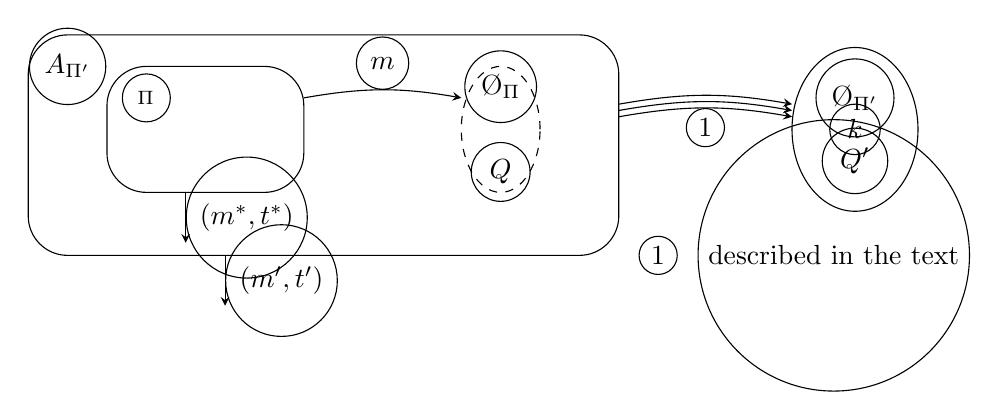
\begin{tikzpicture}[x=1cm, y=0.8cm]
		\draw[rounded corners=0.5cm] (-0.5, 0) rectangle (7, 3.5);
		\draw[rounded corners=0.5cm] (0.5, 1) rectangle (3, 3);
		\draw[dashed] (5.5, 2) ellipse (0.5 and 1);
		\draw (10, 2) ellipse (0.8 and 1.3);
		\draw[-stealth] (3, 2.5) to[bend left=10] node[midway, above] {$m$} (5, 2.5);
		\draw[-stealth]
			(7, 2.4) edge[bend left=10] (9.2, 2.4)
			(7, 2.3) edge[bend left=10] (9.2, 2.3)
			(7, 2.2) to[bend left=10] node[midway, below, draw, circle, inner sep=2pt] {1} (9.2, 2.2)
		;
		\draw[-stealth]
			(1.5, 1) edge node[midway, right] {$(m^*, t^*)$} (1.5, 0.2)
			(2, 0) -- node[midway, right] {$(m', t')$} (2, -0.8)
		;
		\draw
			(1, 2.5) node {$\A_\Pi$}
			(0, 3) node {$A_{\Pi'}$}
			(5.5, 2.1) node[above] {$\O_\Pi$}
			(5.5, 1.8) node[below] {$Q$}
			(10, 2.5) node {$\O_{\Pi'}$}
			(10, 2) node {$k$}
			(10, 1.5) node {$Q'$}
			(7.5, 0) node[draw, circle, inner sep=2pt] {1} ++(0.5, 0) node[right] {described in the text}
		;
		\end{tikzpicture}
		\item $\A'$ should pick a random $r\leftarrow \{0,1\}^{\frac{n}{4}}$, parse m into d blocks $m_1,...,m_d$ and send to its oracle $d$ queries $r\|l\|i\|m_i$ for $i = 1, \ldots, d$.
		After the $d$ queries made to its oracle $O'$, $\A'$ computes $\langle r, t_1, \ldots, t_d \rangle$ where $t_i$ is the answer of the oracle to its $i$th query. He then sends it as an answer to $\A$s query.
		\item For $\Pi$, a forgery is a pair $(m, \langle r, t_1, \ldots, t_d \rangle)$ where $m$ has not been queried before
		and $t_i = \Mac'_k(r\|l\|i\|m_i)$ for $i = 1, \ldots, d$ where $l$ is the length of $m$ and $m = m_1\| \cdots \|m_d$.
		\begin{itemize}
			\item
			If none of its previous query has the same $r$ and $l$, $r\|l\|1\|m_1$ cannot be a query made by $\A'$ and
			$(r\|l\|1\|m_1, t_1)$ is an existential forgery for $\Pi'$ that $\A'$ can output.
			\item
			If 2 previous queries have both $r$ and $l$, then we do not necessarily have an existential forgery.
			However, since $r$ is picked at random ($\A'$ could cheat and make sure that the same $r$ is not picked twice)
			the probability (birthday paradox) of this to happen (if all $m$ have the same $l$ which is the worst case) is approximately
			$\frac{q(n)^2}{2 \cdot 2^n}$ where $q(n)$ is the number of queries made by $\A$.
			\item
			If one unique previous query $m^j$ has this $r$ and $l$, since $m$ is not one of the previous query, there must be $i$
			such that $m_i \neq m_i^j$.
			We know therefore that $r\|l\|j\|m_j$ has never been queried by $\A'$ so $(r\|l\|j\|m_j, t_j)$ is an existential forgery for $\Pi$.
		\end{itemize}
		\item In conclusion, we have
		\begin{align*}
			\Pr[\MacForge_{\A,\Pi}(n) = 1]
			& \leq \Pr[\MacForge_{\A',\Pi'}(n) = 1] + \frac{q(n)}{2^{n+1}}\\
			\epsilon(n)
			& \leq \epsilon'(n) + \frac{q(n)}{2^{n+1}}
		\end{align*}
		so since $\epsilon'(n)$ and $\frac{q(n)}{2^{n+1}}$ are negligible,
		$\epsilon(n)$ is negligible.
	\end{enumerate}

	Alternative answer:
	\begin{enumerate}[start=2]
		\item When $\A_\Pi$ asks for $\Mac_k(m)$, we ($\A_{\Pi'}$) should parse $m=m_1||m_2||\dots||m_d$ with $|m_i|=\frac{n}{4} \, \forall 1\le i \le d=\lceil \frac{l}{n/4}\rceil$ and with the message zero-padded.

		Pick $r \pick \bset^{n/4}$.

		Then, do $d$ requests to $\O_{\Pi'}$ to build $t_i \define \Mac'_k(r||l||i||m_i) \, \forall 1 \le i \le d$.

		Finally, send $t=\langle r, t_1, \dots, t_d\rangle$ to $\A_\Pi$.

		An important question to answer is whether this operation keeps $\A_{\Pi'}$ PPT, with so much requests. To prove this, observe that 1) the message $m$ is generated by a PPT adversary so 2) its length must be polynomial and 3) there is thus at most a polynomial number of blocks and thus 4) we only do a polynomial number of requests to $\O_{\Pi'}$ when $\A_\Pi$ does a request to $\O_\Pi$. So, we are still PPT.

		\item When $\A_\Pi$ outputs $(m^*, t^*)$, we have $t^*=\langle r, t_1, \dots, t_d\rangle$ with $t_i=\Mac'_k(r||l||i|m_i^*)$.

		By hypothesis, there is a chance of $\negl(n)$ that $(m^*, t^*)$ is valid and $m^*$ has never been requested to $\O_\Pi$, i.e., us. Now, we need to extract a valid $(m', t')$ for $\Pi'$. There are three cases:
		\begin{itemize}
			\item If the pair $(r, l)$ has never been used in any of our requests, then $r||l||i||m_i^*$ has never been queried to $\O_{\Pi'}$, and we have our forgery: take any of $(r||l||i||m_i^*, t_i)$.
			\item If $(r, l)$ has been used before, then we need to distinguish between two cases. The first case is if $r$ has been used two or more times before: as $r$ is picked randomly, this event happens with probability $\frac{q(n)}{2^{n/4}}$. In that case, for correct $l$, $\A_\Pi$ could have just rearranged blocks from two previous messages $m^1$ and $m^2$ to build a new message $m^*$. For him, this is an existential forgery against $\Pi$. But for us, all those blocks $r||l||i||m_i^{1, 2}$ have been queried to our oracle before, and so none of them are fresh, and this is not a forgery against $\Pi'$.
			\item If $(r, l)$ has been used before and $r$ has only been used once, then there is a past message $m^1$ whose tag used this $r$. Let's compare the two messages:
			\begin{align*}
			m^1 &\rightarrow m_1^1||m_2^1||\dots||m_d^1 \rightarrow \langle r, \Mac'_k(r||l||1||m_1^1), \dots\rangle \\
			m^* &\rightarrow m_1^*||m_2^*||\dots||m_d^* \rightarrow \langle r, \Mac'_k(r||l||1||m_1^*), \dots\rangle
			\end{align*}
			As $m^*$ is a forgery against $\Pi$, $m^1 \neq m^*$, so $\exists j \suchthat m_j^1 \neq m_j^*$. For this $i$, the corresponding $(r||l||j||m_j^*, t_j)$ is a forgery against $\Pi'$.
		\end{itemize}
		If now we compute it,
		\begin{align*}
		\negl'(n) = \Pr[\MacForge_{\A_{\Pi'},\Pi'}(n)=1] &\ge \Pr[\MacForge_{\A_\Pi,\Pi}(n)=1 \\
		&\quad \wedge \text{ We can build a forgery from it}] \\
		&\ge \Pr[\MacForge_{\A_\Pi,\Pi}(n)=1] \cdot \left(1-\frac{q(n)}{2^{n/4}}\right) \\
		&= \negl(n) \left(1-\frac{q(n)}{2^{n/4}}\right)
		\end{align*}
		As we know that $\Pi'$ is EUF-CMA, then $\negl'(n)$ must be negligible, so the whole right-hand side must be negligible too, and so $\negl(n)$ must be negligible.

		Other said, if $\negl(n)$ is non-negligible, then the right-hand side is non-negligible (the term in parenthesis is negligibly close to $1$), and so $\negl'(n)$ must be non-negligible too.
	\end{enumerate}
\end{solution}



\subsection{Exercise 3 (Authenticated encryption and sPRP)}

\copypaste{4}{2}



\subsection{Exercise 4 (Authenticated encryption)}

Let $\Pi=(\Gen, \Enc, \Dec)$ be an authenticated encryption scheme where $0\not\in \C$ (that is, the string ``0'' is not a possible ciphertext for $\Pi$). Consider the following scheme $\Pi' \define (\Gen', \Enc', \Dec')$ with:
\begin{itemize}
	\item $\Gen'=\Gen$
	\item $\Enc'=\Enc$
	\item $\forall k: \Dec'(c) = \begin{cases} \Dec(c) \text{ if } c\neq 0, \\ 0 \text{ if } c=0. \end{cases}$
\end{itemize}
\begin{enumerate}
	\item Is $\Pi'$ unforgeable?
	\item Is $\Pi'$ CCA secure?
\end{enumerate}


\begin{solution}
	\begin{enumerate}
		\item It is not unforgeable. To see this, simply build the following adversary $\A$:
		\begin{enumerate}[label=(\arabic*)]
			\item The oracle-challenger chooses $k \pick \K$.
			\item We have no query to do to the oracle.
			\item Output $c=0$.
		\end{enumerate}
		By definition, $\Dec'_k(0)=0 \, \forall k$, so it is a valid message. So $\Pr[\EncForge_{\A, \Pi'}(n)=1]=1$.
		\item It is CCA-secure (sure at 95\%). To show this, let's do a reduction. If we have a PPT adversary $\A_{\Pi'}$ against $\Pi'$, we can build an adversary $\A_\Pi$ against $\Pi$ and run the following experiment (from the viewpoint of $\A_\Pi$):
		\begin{enumerate}[label=(\arabic*)]
			\item The oracle-challenger chooses $k \pick \K$.

			\item First query phase:
			\begin{itemize}
				\item When $\A_{\Pi'}$ asks for $\Enc'_k(m)$ of a message $m$, we simply forward the request to $\O_\Pi$, receive $c=\Enc_k(m)$, and return it to $\A_{\Pi'}$
				\item When $\A_{\Pi'}$ asks for $\Dec'_k(c)$ of a ciphertext $c$, if $c=0$, then we return $0$, and if $c\neq 0$, we forward the request to $\O_\Pi$, receive $m=\Dec_k(c)$ and return it to $\A_{\Pi'}$.
			\end{itemize}

			\item $\A_{\Pi'}$ outputs its messages $m_0, m_1$. We output them.

			\item The challenger-oracle picks $b\pick \bset$, returns $c^*=\Enc_k(m_b)$, sends that to us, and we forward it to $\A_{\Pi'}$.

			\item Second query phase, similar to the first one, with the exception that $\A_{\Pi'}$ cannot ask for $\Dec'_k(c^*)$.

			\item $\A_{\Pi'}$ outputs its guess $b'$, and we output $b''=b'$.
		\end{enumerate}
		The adversary $\A_{\Pi'}$ is exactly in the correct conditions, our adversary $\A_\Pi$ is PPT, and we output the same value, so $\Pr[\PrivKcca[\A_\Pi, \Pi](n)=1]=\Pr[\PrivKcca[\A_{\Pi'}, \Pi'](n)=1]=\Pr[b'=b]=\Pr[b''=b]=\negl$
		and, as we know that $\Pi$ is CCA-secure, then we have that $\Pi'$ is CCA-secure. This ``zero-filling'' has no impact on the CCA-security, only on the unforgeability.
	\end{enumerate}
\end{solution}



\subsection{Exercise 5}
% This practical session was entirely corrected by the teaching assistants so, there is no need to correct the solutions.

Let $F$ be a PRF. Below, we describe three \textit{insecure} \emph{variable-length} message authentication codes (\textit{a.k.a.} MACs), $\Pi_1$, $\Pi_2$ and $\Pi_3$, which all use the same key generation algorithm $\G$. The message space is \emph{any (non negative) number} of message blocks in $\{0,1\}^n$, where $n$ is the security parameter.
%
\begin{description}
	\item[$\G(1^n)$] outputs a random key $k\gets\bset^n$.
\end{description}
%
The scheme $\Pi_3$ is built from $\Pi_2$ which is itself built from $\Pi_1$ as an (unsuccessful) attempt to ``patch'' the previous scheme:
%
\begin{description}
	\item[$\Pi_1=(\Gen,\Mac^1,\Vrfy^1)$:]
	\emph{``Deterministic MAC -- Chaining PRFs''}

	$\Mac^1_k(m_1,\ldots,m_\ell)$ computes $t_1=F_k(m_1)$ as well as
	$t_i=F_k(m_i\oplus t_{i-1})$, for $i=2$ to $\ell$, and returns $t \define t_\ell$ (note that only the last block is returned).

	$\Vrfy^1_k((m_1,\ldots,m_{\ell}),t)$ outputs $1$ if
	$\Mac^1_k(m_1,\ldots,m_{\ell})=t$, and 0 otherwise.
	\item[$\Pi_2=(\Gen,\Mac^2,\Vrfy^2)$:]
	\emph{``Padding a random message block in the end''}

	$\Mac^2_k(m_1,\ldots,m_\ell)$ first picks a random $r\gets\{0,1\}^n$ and
	then runs $t=\Mac_k^1(m_1,\ldots,m_\ell,r)$ and outputs $(r,t)$.

	$\Vrfy^2_k((m_1,\ldots,m_{\ell}),(r,t))$ outputs $1$ if
	$\Mac^1_k(m_1,\ldots,m_{\ell},r)=t$, and 0 otherwise.

	\item[$\Pi_3=(\Gen,\Mac^3,\Vrfy^3)$:]
	\emph{``Padding a random message block in the beginning''}

	$\Mac^3_k(m_1,\ldots,m_\ell)$ first picks a random $s\gets\{0,1\}^n$ and
	then runs $(r,t)=\Mac_k^2(s,m_1,\ldots,m_\ell)$ and outputs $(r,s,t)$.

	$\Vrfy^3_k((m_1,\ldots,m_{\ell}),(r,s,t))$ outputs $1$ if
	$\Mac^1_k(s,m_1,\ldots,m_{\ell},r)=t$, and 0 otherwise.
\end{description}

\begin{enumerate}
	\item Describe $\Mac_k^3(m_1,\ldots,m_\ell)$ explicitly in term of computations
	of $F_k$ (and $\oplus$ of course).
	\item Show the correctness of $\Pi_3$.
	\item Mount a forgery attack on these MACs.
\end{enumerate}

\begin{solution}
	\begin{enumerate}
		\item For random $r,s\leftarrow \{0,1\}^n$,
		$\Mac^3_k(m_1,\ldots,m_\ell)$ computes $t_0=F_k(s)$, then $t_i=F_k(m_i \oplus t_{i-1})$ for $i=1$ to $\ell$, and finally
		$t_{\ell+1}=F_k(r\oplus t_\ell)$.
		It outputs $(r,s,t)$ where $t \define t_{\ell+1}$.

		\item Using the description of $\Mac^1_k$, on inputs $(s,m_1,\ldots,m_\ell,r)$ it gives $t'_1=F_k(s)$, for $i=1$ to $\ell$, $t'_{i+1}=F_k(m_i \oplus t'_i)$, and $t'_{\ell+2}=F_k(r \oplus t'_{\ell+1})$. $t'_{\ell+2}$ is the output, or equivalently:
		\begin{align*}
		F_k(r \oplus t'_{\ell+1}) &= F_k \bigg(r \oplus F_k \Big(m_\ell \oplus F_k \big( m_{\ell-1} \oplus \dots F_k(m_1\oplus F_k(s)) \dots \big)\Big)\bigg)\\
		&=t.
		\end{align*}

		\item These MACs are not even one-time secure:
		\begin{description}
			\item $\Pi_1$: (1) query $\Mac^1_k(m)$ on any $m\in\bset^n$ and get the tag $t=F_k(m)$;

			(2) output $((m,m\oplus t),t)$.

			$t_1=F_k(m)$, $t_2=F_k(m\oplus t \oplus t_1)= F_k(m \oplus 0)=t$.

			\item $\Pi_2$: (1) query $\Mac^2_k(m)$ on any $m\in\{0,1\}^n$ and get the tag $(r,t)$, where $t=F_k(F_k(m)\oplus r)$;

			(2) output $((m,r,m\oplus t),(r,t))$.

			$t_1=F_k(m)$, $t_2=F_k(F_k(m)\oplus r)=t$, $t_3=F_k(t\oplus m \oplus t)=F_k(m)$, $t_4=F_k(F_k(m)\oplus r)=t$.

			\item $\Pi_3$: (1) query $\Mac^3_k(m)$ on any $m\in\{0,1\}^n$ and get the tag $(r,s,t)$, where $t=F_k( F_k(F_k(s) \oplus m)  \oplus r)$

			(2) output $((m,r,s\oplus t,m),(r,s,t))$.

			$t_1=F_k(s)$, $t_2=F_k(F_k(s) \oplus m)$, $t_3=F_k(F_k(F_k(s) \oplus m) \oplus r)=t$, $t_4=F_k(t \oplus s \oplus t)= F_k(s)$, $t_5=F_k(F_k(s)\oplus m)$, $t_6=F_k( F_k(F_k(s) \oplus m)  \oplus r)=t$.
		\end{description}
	\end{enumerate}
\end{solution}



\subsection{Exercise 6}
% This practical session was entirely corrected by the teaching assistants so, there is no need to correct the solutions.

Let $F$ be a pseudorandom function, $G$ be a pseudorandom permutation, $T$ be a public $n$-bit constant, $k$ be a $n$-bit secret key, $m$ be a $n$-bit message, $IV$ be a $n$-bit random value chosen by the party computing the encryption (resp.~MAC) before each operation. Among the following constructions, determine the ones that would be acceptable and justify your answer. (Your justifications can rely on results that have been presented during the class.)

\begin{enumerate}
	\item $\Enc_k(m) \define F_k(m \oplus T)$ as an encryption scheme secure against
	eavesdropping.

	\item $\Enc_k(m) \define G_k(m \oplus T)$ as an encryption scheme secure against eavesdropping.

	\item $\Enc_k(m) \define G_k(m \oplus T)$ as an encryption scheme secure against a CPA-adversary.

	\item $\Enc_k(m) \define (IV,G_k(m \oplus T \oplus IV))$ as an encryption scheme secure against a CPA-adversary.

	\item $\Mac_k(m) \define F_k(m \oplus T)$ as a MAC scheme existentially unforgeable under an
	adaptive chosen-message attack.

	\item $\Mac_k(m) \define (IV,G_k(m\oplus IV \oplus T))$ as a MAC scheme
	existentially unforgeable under an adaptive chosen-message attack.
\end{enumerate}


\begin{solution}
	\begin{enumerate}
		\item No, decryption does not work in general, as we do not
		necessarily know how to invert a PRF.

		\item 	Yes, it is secure.  The reduction to the PRP security can work as follows:
		the reduction gets $m_0$ and $m_1$ from the eavesdropper
		adversary, picks a random bit $b$, sends $m_b \oplus T$ to the
		challenger and receives a value $c$ that it sends back to the eavesdropper
		adversary. This adversary has a probability exactly $1/2$ to
		guess $b$ if $c$ comes from a random permutation, and a
		probability $1/2 + \negl$ to guess $b$ if $c$ comes from a
		pseudorandom permutation. The reduction can therefore claim that
		it sees a PRP every time the adversary makes a successful
		guess. The difference between the two probabilities is $\negl$.
		So, if $F$ is a PRP, $\epsilon$ must be negligible.

		\item 	No: it is not probabilistic. CPA security is not achievable with deterministic encryption.

		\item We first observe that the $\oplus T$ does not matter:
		since $T$ is public, the adversary has the possibility to adapt
		its choice of $m$ in order to cancel it.  Now, if we abstract
		from $T$, this is exactly the CBC encryption mode, which we know
		to be CPA-secure.

		\item Again, we observe that the $\oplus T$ does not matter: since
		$T$ is public, the adversary has the possibility to choose exactly
		on which value $F_k$ will be applied. Now, if we abstract from $T$,
		this is exactly the basic MAC scheme from the class, which is secure.

		\item This is insecure. Given one tag $(IV, t)$ on a message
		$m$, the adversary can produce a valid tag $(IV', t)$ on the
		message $m' = m \oplus IV \oplus IV'$ for any $IV'$.
	\end{enumerate}
\end{solution}



\subsection{Exercise 7 (Blue-ray security)}

The movie industry wants to protect digital content distributed on DVD's. We study
one possible approach. Suppose there are at most a total of $n$ DVD players in the world (e.g.
$n=2^{32}$). We view these n players as the leaves of a binary tree of height $\log_2 n$.
Each node $\nu_j$ in this binary tree contains an AES key $K_j$ such that
$\mathrm{Enc}_{K_j}:\{0,1\}^l\rightarrow\{0,1\}^l$ is assumed to be a \emph{secure} encryption.
These keys are kept secret from consumers and are fixed for all time.
At manufacturing time each DVD player is assigned a serial number $i\in\left[0,n-1\right]$.
Consider the set $S_i$ of $\log_2(n+1)$ nodes along the path from the root to leaf number
$i$ in the binary tree. The manufacturer of the DVD player embeds in player number $i$ the
$\log_2(n+1)$ keys associated with the nodes in $S_i$. In this way each DVD player ships with
$\log_2(n+1)$ keys embedded in it (these keys are supposedly inaccessible to consumers).

\begin{enumerate}
	\item Since all DVD players have the key \emph{root} (noted $K_{root}$),
	      find a way to protect the content $M\in\{0,1\}^l$ of a DVD such that all players can decrypt
	      the movie (and then read it).
	\item Now suppose that a hacker has been able to extract the key $K_{root}$ embedded in his
	      DVD player and has published it on the Internet.
	      Show how the movie industry can encrypt the contents of a new DVD $M\in\{0,1\}^l$ such that only
	      the owners of a DVD player can read it.
	      Note that the movie indutry does not want to produce several encryptions of the
	      same content $M$ \emph{i.e.} there will be a single manner to protect the DVD.
	\item Suppose the $\log_2n$ keys embedded in DVD player number $r$ are exposed by hackers
	      and published on the Internet. Show that when the movie industry is about to
	      distribute a new DVD movie they can encrypt the contents of the DVD using a
	      ciphertext of size $l\!\cdot\!(1+\log_2n)$ so that all DVD players can decrypt the movie except
	      for player number $r$. In effect, the movie industry disables player number $r$.

	      \emph{Hint: the DVD will contain $\log_2n$ ciphertexts where each ciphertext is the
	      encryption of a unique K under certain $\log_2n$ keys from the binary tree.}
\end{enumerate}


\begin{solution}
  \begin{enumerate}
    \item Encrypt all the DVDs with $K_\text{root}$, i.e. build the ciphertext: $c_{root}=Enc_{K_{root}}(M)$
    \item At the beginning of the DVD, encrypt a random key $K$ twice (using $K_2$ and then $K_3$): $Enc_{K_2}(K)$ and $Enc_{K_3}(K)$.

      We then encrypt all the content $M$ of the DVD using $K$. (We suppose $K_1$ is $K_{\text{root}}$)
      $K_2$ and $K_3$ are the keys associated to the 2 childs of the root.

      \textbf{Other possibility}

      Simply encrypt the contents of the new DVD M as: $Enc_{K2}(M)||Enc_{K3}(M)$. This way, each DVD player is still able to decrypt the content, but nobody that only has $K_{root}$.
    \item
      For every node $i$ on the path from the root to $r$, we must add an encryption of $K$ with the key of its child that is not in the path.
      For example, if $r = 10$ and $n = 16$, we must include the bold keys,
      so we will include the encryption of $K_7$ in a DVD which is quite something.

      \textbf{Expressed differently}

      If we want to disable the DVD player 11 for example, we can create a new ciphertext as: $c_{disable} = Enc_{K_2}(M)||Enc_{K_7}(M)||Enc_{K_{12}}(M)||Enc_{K_{player10}}(M)$

      \begin{center}
        \Tree [.{$K_{\text{root}} = K_1$}
          [.{$\mathbf{K_2}$}
            [.{$K_4$}
              [.{$K_8$}
                [.{0} ]
                [.{1} ]
              ]
              [.{$K_9$}
                [.{2} ]
                [.{3} ]
              ]
            ]
            [.{$K_5$}
              [.{$K_{10}$}
                [.{4} ]
                [.{5} ]
              ]
              [.{$K_{11}$}
                [.{6} ]
                [.{7} ]
              ]
            ]
          ]
          [.{$K_3$}
            [.{$K_6$}
              [.{$\mathbf{K_{12}}$}
                [.{8} ]
                [.{9} ]
              ]
              [.{$K_{13}$}
                [.{\textbf{10}} ]
                [.{11} ]
              ]
            ]
            [.{$\mathbf{K_7}$}
              [.{$K_{14}$}
                [.{12} ]
                [.{13} ]
              ]
              [.{$K_{15}$}
                [.{14} ]
                [.{15} ]
              ]
            ]
          ]
        ]
      \end{center}
  \end{enumerate}
\end{solution}



\subsection{Exercise 8 (Authenticated encryption, or not)}

\copypaste{10}{1}



\subsection{Exercise 9 (Authenticated encryption)}

\copypaste{4}{1}



% TODO
\subsection{Exercise X (Mode of operation)}
Show formally that ECB-mode encryption does not have indistinguishable encryptions in the presence of an eavesdropper.
\begin{solution}
  Let say we have to split the message into $m$ messages of $n$ bits.
  Choosing $m_0 = M_0 \| M_0 \| \cdots \| M_0$ and $m_1 = M_1 \| M_2 \| \cdots \| M_m$ with $M_i \neq M_j$ for $i \neq j$,
  if $b = 0$, $\A$ will get $c = C_0 \| C_0 \| \cdots \| C_0$ for some $C_0 \in \C$. But if b=1, $\A$ will get $c = C_1 \| C_2 \| \cdots \| C_m$ for some $C_i \in \C$.

  An adversary $\A$ can output $b = 0$ iff all the $C_i$s are equals.
  We have
  \[ \Pr[\PrivK^{\text{eav}}_{\A,\text{ECB}}(nm)] = \frac{1}{2} + \frac{1}{2} = 1 \]
  since the $C_i$ cannot be equal if $b = 1$ since we use a PRP.
  If two different $M_i$ were encrypted as same $C_i$, decryption wouldn't be possible.
\end{solution}

\section{}
\subsection{Exercise 0 (Group order)}
\copypaste{3}{5}

\subsection{Exercise 1 (ElGamal Public Key Encryption and CCA Security)}
\begin{enumerate}
	\item Write the security definition of CCA security for a public key encryption scheme.
	\item Let $(c_1,c_2)$ and $(c_1',c_2')$ be two ElGamal ciphertexts, of plaintext $m$ and $m'$ respectively. Can $(c_1 c_1',c_2 c_2')$ be a ciphertext relatively to this scheme? 
	\item From $(c_1,c_2)$ a ciphertext of $m$, can you build another ciphertext valid for $m$ (remember that the public key is $(\mathbb{G},g,q,h=g^x)$)? If yes, what is its decryption? 

	\item Show that ElGamal Public Key Encryption is not CCA secure.
\end{enumerate}
\begin{solution}
\begin{enumerate}
    \item 
    Given  $\Pi := \langle$ Gen, Enc, Dec$\rangle$, and adversary $A$, define the following experiment $\text{ PrivK}^{cca}_{A, \Pi}$ : 
    \begin{enumerate}
        \item Gen probabilistically selects ($pk$, $sk$) $\leftarrow$ Gen(1$^n$). $pk / sk$ are the public/private key.
        \item $A$ is given oracle access to $Dec_{sk}(\cdot)$.
        \item $A$ outputs $m_0, m_1$ of same length.
        \item Choose $b \leftarrow$ \{0, 1\}, and send $c := Enc_{pk}(m_b)$ to $A$.
        \item $A$ is again given access to $Dec_{sk}(\cdot)$ but he cannot ask $Dec_{sk}(c)$.
        \item $A$ outputs $b'$.
        \item Define $\text{PrivK}^{cca}_{A, \Pi}(n) := 1$ iff $b=b'$
    \end{enumerate}
    $\Pi := \langle$ Gen, Enc, Dec$\rangle$ is CCA-secure for a public key encryption scheme if $\forall$ PPT $A, \exists \epsilon$ :
    $$ Pr[\text{ PrivK}^{cca}_{A, \Pi}(n)] \leq \frac{1}{2} + \epsilon(n) $$
    
    \item (c$_1$c$_1$', c$_2$c$_2$') is a valid ciphertext for the message : m $\cdot$ m'. \newline
    We can prove this like : 
    $$Dec_{sk}(c_1c_1',c_2c_2') = \frac{c_2c_2'}{c_1^xc_1'^x} = \frac{mh^{y_1}m'h^{y_2}}{g^{xy_1}g^{xy_2}} = m \cdot m'$$
    
    \item Yes, if we think about this property : $m \cdot 1 = m$ and we combine it with the property found last exercise : $Dec_{sk}(c_1c_1',c_2c_2') = m \cdot m'$, it is easy to produce a new valid ciphertext. \newline
    If we compute $Enc_{pk}(1) := (c_1', c_2')$ (we can do it since we are in a \textbf{public key encryption scheme}), the ciphertext (c$_1$c$_1$', c$_2$c$_2$') will be a valid ciphertext and its decryption will give : m.
    \newline
    \textbf{Other possibility} \newline
    We can also simply choose $y' \leftarrow \mathbb{Z}_q$ and build the ciphertext $(c_1.g^{y'},c_2.h^{y'})=(g^{y+y'},m.g^{x(y+y')})$. The decryption gives m.
    
    \item Now, we are able to see why ElGamal does not hold CCA-security with the 2 properties found. \newline
    If the adversary $A$, after received $c := (c_1, c_2)$, compute $Enc_{pk}(1) := (c_1', c_2')$ and make the following oracle access $Dec_{sk}(c_1c_1',c_2c_2') := m_x$, he will now be able to (really) easily determine b from $m_x$. Then we can say that :
    $$ Pr[\text{ PubK}^{cca}_{A, ElGamal}(n)] = 1$$
    Which means ElGamal does not hold CCA-security with public key encryption.
    \newline
    \textbf{Other possibility} \newline
    We build an attacker A as follows : 
    \begin{enumerate}
        \item A outputs $m_0$, $m_1$ $\in M$.
        \item A receives $(c_1,c_2)=Enc_{pk}(m_b)=(g^y,m_b.g^{xy})$
        \item A queries the decryption of the transformed ciphertext $(c_1.g^{y'},c_2.h^{y'})$ for some arbitrary chosen y' from $\mathbb{Z}_q$, and receives directly $m_b$ as a response from his oracle.
    \end{enumerate}
\end{enumerate}
\end{solution}

\subsection{Exercise 2 (ElGamal in \texorpdfstring{$QR_p$}{QRp})}
Let $p=2q+1$ with $q$ prime, let $\mathbb{G}=QR_p$ the group of squares modulo $p$, and $g$ be a generator of $\mathbb{G}$. 
We define ElGamal encryption scheme in this group: The private key is $(\mathbb{G},g,q,x)$, the public key is $(\mathbb{G},g,q,h=g^x)$
where $x \in \mathbb{Z}_{q}^*$ is chosen uniformly. To encrypt a message $m$ $\in \mathbb{Z}_{q}$, choose a uniform $r \in \mathbb{Z}_{q}$, compute $c_1=g^r \mod p$ and $c_2=h^r+m \mod p$ and let the ciphertext be $(c_1,c_2)$.

\begin{enumerate}
	\item What is the order of $g$?
	\item Is this scheme CPA-secure? 

	
\end{enumerate}
\begin{solution}
\begin{enumerate}
    \item As g is a generator of $\mathbb{G}$, then ord(g)=$|\mathbb{G}|$. According to \ref{subsec:4.6} and given the fact that $\mathbb{G}$ := $QR_p$, then $|\mathbb{G}| = \frac{p - 1}{2} = q =$  ord(g).
    \item The scheme is CPA-Secure and we gonna prove it by assuming that $QR_p$ holds in DDH. \newline
    Let's build a PPT adversary $\A$ which can solve $ElGamal$ in $QR_p$ with an advantage $\eta$. It works like this :
    \begin{enumerate}
        \item We send pk to $\A$ where pk = ($\mathbb{G}$, g, q, h = $g^x$).
        \item $\A$ does q(n) queries to its oracle.
        \item $\A$ is then doing the challenge : it outputs $m^*_0$, $m^*_1$ and send it to its $ElGamal$ oracle. 
        \item The $ElGamal$ oracle picks a random $b \in \{0, 1\}$ and sends back $Enc_{pk}(m_b) = (c_1^b, c^b_2)$  to $\A$
        \item $\A$ then outputs $b'$.
    \end{enumerate}
    We will use $\A$ to build a distinguisher $\D$ able to solve $DDH_{\D, \mathbb{G}}(n)$ : 
    \begin{enumerate}
        \item Run $\mathbb{G}$(n) to obtain ($\mathbb{G}$, q, g). 
        \item We choose (x, y, z) $\xleftarrow{R} \mathbb{Z}^3_q$.
        \item We set $h_1 = g^{x \cdot y}$, $h_0 = g^{z}$ and $b'' \leftarrow \{0, 1\}$. We forward then $((\mathbb{G}, q, g), (g^x, g^y, h_{b''}))$ to $\D$.
        \item $\D$ will then build $pk  = (\mathbb{G}, q, g, g^x)$ and will forward $pk$ to $\A$.
        \item $\A$ will then output its challenge queries $m^*_0$, $m^*_1$. $\D$ will pick $b \leftarrow \{0, 1\}$, and produce $c_b = (c_1^b, c^b_2) = (g^y, h_{b''} + m_b \text{ mod p})$. It will then forward $c_b$ to $\A$.
        \item $\A$ will output $b'$.
        \item $\D$ will output $ 1 \Leftrightarrow b = b'$.
    \end{enumerate}
    We analyse the chance of success to determine $Priv^{cpa}_{\A, ElGamal}$ : 
    \begin{itemize}
        \item if $b'' = 0$, then Pr[$\D$ outputs 1] = $\frac{1}{2}$.
        \item if $b'' = 1$, then Pr[$\D$ outputs 1] = $\frac{1}{2}$ + $\eta(n)$.
    \end{itemize}
    It means that $\D$ will only has advantage $\eta(n)$ to solve DDH. But as it is assumed as hard, we can conclude that $\eta(n)$ is negligible. Therefore, $$Priv^{cpa}_{\A, ElGamal}(n) = \frac{1}{2} + negl(n) $$
    By reduction, we just proved that this scheme is CPA-secure under DDH hardness assumption.
\end{enumerate}
\end{solution}


\subsection{Exercise 3 (A Variation of ElGamal in \texorpdfstring{$PKE$}{PKE})}
\label{subsec:varia-elgamal-pke}
Let consider ElGamal public encryption scheme with Encryption algorithm modified in the following way, where $\mathcal{M}=\{0,1\}$:
\begin{itemize}
	\item If $b=0$ then choose a uniform $y\in \mathbb{Z}_{q}$ set $c_1=g^y$, $c_2=h^y$, and the ciphertext is $(c_1,c_2)$.
	\item If $b=1$ then choose independent uniform $y,z \in \mathbb{Z}_{q}$ set $c_1=g^y$, $c_2=g^z$, and the ciphertext is $(c_1,c_2)$.
\end{itemize}

\begin{enumerate}
	\item How is it possible to decrypt correctly such ciphertexts with the private key?
	\item Show that this scheme is CPA secure if DDH holds in $\mathbb{G}$. 
\end{enumerate}
\begin{solution}
\begin{enumerate}
    \item We can define $Dec_{x}(c_1, c_2)$ as : $\begin{cases}
    1 \textsc{ if } c_2 \neq c_1^x \\
    0 \textsc{ if } c_2 = c_1^x\\
\end{cases}$ \newline \newline
    We observe that Pr[$Dec_{x}(c_1, c_2)$ = 0 $|$ $(c_1, c_2) \leftarrow Enc(0)$] = 1 because the decryption is always correct. \newline \newline
    On the other hand, we observe that Pr[$ Dec_{x}(c_1, c_2) \neq 1$ $|$ $(c_1, c_2) \leftarrow Enc(1)$] = Pr[$ z = xy $] = $\frac{1}{|\mathbb{G}|}$ is negligible, then we conclude that the decryption is correct
    
    \item Assuming the DDH problem is hard in $\mathbb{G}$. \newline
    Assume it exists a PPT adversary $\mathcal{A}$ for $\Pi$, we build a distinguisher D able to break DDH with non negligible probability as follows :
    \begin{enumerate}
        \item Run $(\mathbb{G},g,q) \leftarrow \mathcal{G}(1^n)$\\
        Define $n:=|q|$\\
        Choose uniformly at random $(x,y,z) \leftarrow \mathbb{Z}^3_q$\\
        Choose at random $b\leftarrow\{0,1\}$\\
        Compute $h_1:=g^{xy}\;h_0:=g^z$ and send $(\mathbb{G},g,q,g^x,g^y,h_b)$ to $\mathcal{A}'$
        
        \item $D$ defines $pk = (\mathbb{G},g,q,g^x)$ and sends it to $\mathcal{A}$
        \item $\mathcal{A}$ sends $(m_0,m_1) = (0,1)$ to $D$
        \item $D$ sends $c=(g^y,h_b)$ to $\mathcal{A}$
        \item \textcolor{red}{Olivier : Pas d'accord à partir de là. C'est la probabilité de l'output b' qui varie en fonction de $h_b$ autrement dit b", je mets ma proposition en dessous.} $\mathcal{A}$ outputs $b'$ 
            \begin{itemize}
                \item if $b'=0\Rightarrow h_b=g^{xy}$
                \item if $b'=1\Rightarrow h_b=g^z$
            \end{itemize}
            $D$ outputs $b''=\Bar{b'}$
        \item Define : $$\text{PubK}^\text{cpa}_{\mathcal{A},\Pi}(n) = 1 \Leftrightarrow b'\neq b$$ $$\text{DDH}_{\mathcal{A}',\mathcal{G}}(n) = 1 \Leftrightarrow b''=b$$
    \end{enumerate}
    If we run the experiment, we have :
    \begin{align*}
        \text{Pr}[\text{PubK}^\text{cpa}_{\mathcal{A},\Pi}(n) = 1] &= \frac{1}{2}+\epsilon(n)\\
        &= \text{Pr}[b'\neq b]\\
        &= \text{Pr}[b''=b]\\
        &= \text{Pr}[\text{DDH}_{\mathcal{A}',\mathcal{G}}(n) = 1]
    \end{align*}
    If $\epsilon(n)$ is non negligible, $\mathcal{A}'$ is a PPT adversary that can break DDH with non negligible probability, which contradicts the assumption. Therefore $\mathcal{A}$ is CPA secure if DDH is hard in $\mathbb{G}$.
\end{enumerate}

\textcolor{red}{Solution} \newline
\begin{enumerate}
    \item D outputs 1 $\Leftrightarrow b'=1$.
    \item We observe : \newline
    If $b=0 \Rightarrow Pr[D outputs 1]=\frac{1}{2}$ (as $g^z$ looks random in $\mathbb{G}$) \newline
    If $b=1 \Rightarrow Pr[D outputs 1]=\frac{1}{2}+\eta(n)$.
    \item We thus have D distinguishing between $g^z$ and $g^{xy}$ with advantage $\eta(n)$. As we assume that DDH holds in $\mathbb{G}$, $\eta(n)$ must be negligible and this scheme is CPA-secure.
\end{enumerate}

\end{solution}

\subsection{Exercise 4 (Authenticated Encryption)}
Consider the following scheme $\Pi=(\Gen,\Enc,\Dec)$ based on the strong pseudorandom permutation $\F:\mathcal{K} \times \lbrace 0,1 \rbrace^n$, defined as follow:
\begin{itemize}
\item $\mathcal{M}=\lbrace 0,1\rbrace^{\frac{n}{2}}$ (the message space)
\item $\Gen$ picks a random key $k \in \mathcal{K}$
\item $\Enc_k(m)$ picks a random value $r \in \lbrace 0,1\rbrace^{\frac{n}{2}}$, and computes $c \leftarrow \F_k(m \| r)$
\item $\Dec_k(c)$ computes $(m\|r)=\F^{-1}_k(c)$ and outputs $m$ (the first half).
\end{itemize}
Answers the following questions:
\begin{itemize}
\item is $\Pi$ unforgeable?
\item is $\Pi$ CCA-secure? (\emph{To do at home})
\item is $\Pi$ an authenticated encryption scheme? (\emph{To do at home})
\end{itemize}



\paragraph{Definition 1} \label{def: sprp} (\emph{Strong PseudoRandom Permutation})

A function $\F:\mathcal{K} \times \mathcal{M} \longmapsto \mathcal{M}$ is a $(q,t,\varepsilon)$-\emph{ strong pseudorandom permutation} ($\sprp$) if for any $(q,t)$-bounded adversary, the advantage:
$$ \mathsf{Adv}^{\sprp}_{\adv}:=
\left| \Pr\left[ \adv^{\F_k(\cdot),\F_k^{-1}(\cdot)}\Rightarrow 1 \right] -
	\Pr\left[ \adv^{\f(\cdot,\cdot),\f^{-1}(\cdot,\cdot)}\Rightarrow 1 \right] \right| 
\leq \varepsilon $$
with $k$  and $\f$ picked uniformly at random from their domains, respectively $\mathcal{K}$ and the set of permutations $\mathcal{M} \rightarrow \mathcal{M}$.
\begin{solution}
\begin{enumerate}
    \item It is not unforgeable because since $F_k$ is a PRP, it is bijective. 
    \newline Then $\forall u \in \{0, 1\}, F_k^{-1}(u) = (u_1 || u_2)$ and $EncForge_{\A, \Pi} = 1$.
    \item It is CCA-secure and we will prove it by assuming that the PRP F is strong. 
    If we build the distinguisher $\D$ using the PPT adversary $\A$ capable of breaking the scheme $\Pi$ with advantage $\eta(n)$. At the start of the game, a random key k and a random bit b are picked by the oracle.
    \begin{enumerate}
        \item When $\A$ asks for the encryption of message $m_i$, $\D$ picks a random $r_i \leftarrow \{0, 1\}^{\frac{n}{2}}$ and queries its oracle on input ($m_i || r_i$) obtaining, if b=0 $c_i = f(m_i || r_i)$, else $c_i = F_k(m_i || r_i)$. 
        $\D$ forwards $c_i$ to $\A$. This is repeated for each message $m_i$ issued for the first query phase.
        \newline Also, when $\A$ asks for the decryption of ciphertext $c_i'$, $\D$ queries its oracle on input $c_i'$ obtaining, if b=0 $(m_i'||r_i') = f^{-1}(c_i')$, else $(m_i'||r_i') = F^{-1}_k(c_i')$, which $\D$ forwards to $\A$. This is repeated for each ciphertext $c_i'$ issued for the first query phase
        \item When $\A$ does the challenge query on output $m^*_0$, $m^*_1$ with $|m^*_0| = |m^*_1|=\frac{n}{2}$ and $m^*_0 \neq m^*_1$,  $\D$ picks a random $r^* \leftarrow \{0, 1\}^{\frac{n}{2}}$ and a random $b'\leftarrow \{0, 1\}$. $\D$ queries then its oracle on input ($m^*_b || r^*$) obtaining, if b=0, $c^* = f(m^*_b || r^*)$, else $c^* = F_k(m^*_b || r^*)$.  $\D$ forwards $c^*$ to $\A$.
        \item When $\A$ asks for the encryption of message $m_i$, $\D$ picks a random $r_i \leftarrow \{0, 1\}^{\frac{n}{2}}$ and queries its oracle on input ($m_i || r_i$) obtaining, if b=0 $c_i = f(m_i || r_i)$, else $c_i = F_k(m_i || r_i)$. 
        $\D$ forwards $c_i$ to $\A$. This is repeated for each message $m_i$ issued for the second query phase.
        \newline Also, when $\A$ asks for the decryption of ciphertext $c_i'$, $\D$ queries its oracle on input $c_i'$ obtaining, if b=0 $(m_i'||r_i') = f^{-1}(c_i')$, else $(m_i'||r_i') = F^{-1}_k(c_i')$, which $\D$ forwards to $\A$. This is repeated for each ciphertext $c_i' \neq c$ issued for the second query phase
        \item At the end of the game, $\A$ outputs a bit b''. $\D$ outputs a bit $1 \Leftrightarrow b'' = b'$. 
    \end{enumerate}
    Now, Pr[$\D$] will depend on b : 
    \begin{itemize}
        \item if b = 0, Pr[$\D$ outputs 1] = $\frac{1}{2} + \frac{q(n)}{2^{\frac{n}{2}}}$ ($m||r$ found twice !)
        \item if b = 1, Pr[$\D$ outputs 1] $\leq \frac{1}{2} + \eta(n)$
    \end{itemize}
    We can see that if $F_k(m)$ is replaced by a true random function $f(m)$, the scheme is CCA-secure (since $\frac{q(n)}{2^{\frac{n}{2}}}$ is negligible). \newline \newline
    So now we check if the scheme is insecure, we can distinguish $F_k(m)$ from a true random function. $|Pr[\D^{F_k(\cdot),F_k^{-1}(\cdot)}(1^n)=1]-Pr[\D^{f(\cdot),f^{-1}(\cdot)}(1^n)=1]| \leq \eta(n) - \frac{q(n)}{2^{n/2}}$. Since $F_k(\cdot)$ is a strong PRP, then $\eta(n)$ is negligible and the scheme $\Pi$ is CCA-secure.
    \item Since the scheme $\Pi$ is CCA-Secure but not unforgeable, then it is not an authenticated encryption
\end{enumerate}
\end{solution}


\subsection{Exercise 5 (Authenticated Encryption)}
Let $\Pi=(\Gen,\Enc,\Dec)$ be an authenticated encryption scheme where $ 0 \not \in \mathcal{C}$ (that is, the string $``0"$ is not a possible ciphertext for $\Pi$). Consider the following scheme $\Pi':=(\Gen',\Enc',\Dec')$ with:

\begin{itemize}
\item $\Gen'=\Gen$
\item $\Enc'=\Enc$
\item 	$ \forall k: \left\{ 	\begin{array}{l l}
\Dec'(c)=\Dec(c) &\quad \text{ if } c \neq 0,\\
 0 &\quad  \text{ if } c = 0. 
\end{array} \right.   $ 
%\item $\Dec'(c)=\Dec(c)$ if $c \neq 0$, if $c=0$ $c \neq 0 ~ \forall$ key $k$.
\end{itemize}

\begin{enumerate}
\item Is $\Pi'$ unforgeable?
\item Is $\Pi'$ CCA secure?
\end{enumerate}
\begin{solution}
    \begin{enumerate}
        \item This is CCA-secure, since $\Pi$ is CCA-secure. (Insert proof here but it is 100\% sure it is CCA-secure).
        \item This is not unforgeable. We can forge a new valid ciphertext if the PPT adversary $\A$ outputs 0, then this ciphertext will be considered as valid and Pr[EncForge$_{\A, \Pi'}$(n) = 1] = 1.
    \end{enumerate}
\end{solution}

\subsection{Exercise 6 (Commitment scheme)}
\label{subsec:commit-scheme}
Define the bit-commitment scheme $\langle \G, \Com, \Open \rangle$ with the following PPT 
algorithms :
\begin{itemize}
\item $\Gen(1^n)$ sets $pk$ as $(\PRG,R)$, where
  \begin{itemize}
  \item $\PRG$ is a random generator $\lbrace 0,1 \rbrace^n \longmapsto \lbrace 0,1\rbrace^{3n}$
  \item $R$ is a random $3n$-bit string
  \end{itemize}
\item $\Com_{pk}(b)$ with $b\in\{0,1\}$ provides $(c,d)$ where: 
  \begin{itemize}
  \item $Y$ is an $n$-bit string
  \item  if $b=0$ $c=\PRG(Y)$
  \item if $b=1$, $c=\PRG(Y) \oplus R$
  \item $d=(b,Y)$
  \end{itemize}
\item $\Open_{pk}(c,d)$ outputs $b$ if it can recompute $c$ from $d$ and $pk$, or $\bot$ otherwise
\end{itemize}

\begin{enumerate}
  \item Is this scheme perfectly hiding?
	\item Is this scheme computationaly binding? 	
	\item If the committer choose $R$ is the scheme secure?
\end{enumerate}

\begin{solution}
\begin{enumerate}
    \item To break the hiding property, an adversary would need to enumerate all possible outputs of G (requires $2^n$ steps) if $G(Y) \oplus R \notin \{x | \forall u : x = G(u)\}$. But this kind of event has a negligible chance of probability (Pr = $\frac{|G(Y)|}{|G(Y) \oplus R|} = \frac{2^n}{2^{3n}} = \frac{1}{2^{2n}} \in negl(n)$) so an adversary with an unbounded power of calculation can easily break the property of perfectly hiding.
    \item It is computationally binding because : 
    $$Pr[G(Y) = G(Y') \oplus R] = \frac{2^n\cdot2^n}{2^{3n}} = \frac{1}{2^n} \in negl(n)$$
    Then we have Pr[Com$^{bind}_{\mathrm{A}, \Pi}$] $\leq \epsilon$, and the scheme is computationally secure. 
    \item Not secure, because if $R = G(Y)$, then the opposite player can easily deduce the value of b. If c = 0, b = 1, else b = 0. 
\end{enumerate}
\end{solution}
\section{TP 5}
%\addcontentsline{toc}{section}{TP 5}

% \section*{Rappel}

% \begin{enumerate}
% \item $\forall x \ p(x) \land q(x) \Lleftarrow\!\!\!\!\Rrightarrow (\forall x \ p(x)) \land (\forall x \ q(x))$
% \item $\exists x \ p(x) \vee q(x) \Lleftarrow\!\!\!\!\Rrightarrow (\exists x \ p(x)) \vee (\exists x \ q(x))$
% \item $\neg \exists x \ p(x) \Lleftarrow\!\!\!\!\Rrightarrow \forall x \ \neg p(x)$
% \item $\neg \forall x \ p(x) \Lleftarrow\!\!\!\!\Rrightarrow \exists x \ \neg p(x)$
% \item $(\forall x \ p(x)) \vee (\forall x \ q(x)) \Rrightarrow \forall x \ p(x) \vee q(x)$
% \item $\exists x \ p(x) \land q(x) \Rrightarrow (\exists x \ p(x)) \land (\exists x \ q(x))$
% \item $\exists x \ p(y) \land q(x) \Rrightarrow p(y) \land (\exists x \ p(x))$
% \item $\exists x, y \ p(x, y) \Rrightarrow \exists y, x \ p(x, y)$
% \end{enumerate}


% \newpage


% \section*{Exercices}


\subsection*{Exercice 1}
Expliquez ce qu'est un modèle en logique des prédicats.

    \subsubsection*{Solution}

    Un modèle est une interprétation qui rend toutes les formules vraies.

    Soit un ensemble de formules $B=\{p_1,\dots ,p_n\}$, une interprétation $I$ de B est un \textit{modèle} si et seulement si $\forall p_i \in B:VAL_I(p_i) = \text{True}$

\subsection*{Exercice 2}
Soit l'interprétation suivante:
\begin{center}
\begin{tabular}{r l}
$D_I$ & $= \mathbb{N}$ \\
$val_I(a)$ & $= 0$ \\
$val_I(f)$ & $= $ \ ''succ`` \\
$val_I(P)$ & $= $ \ ''$<$`` \\
$val_I(x)$ & $= 1$ \\
$val_I(y)$ & $= 0$ \\
\end{tabular}
\end{center}
Déterminez les valeurs de vérité des formules suivantes dans cette interprétation:
\begin{enumerate}
\item $P(x, a)$
\item $P(x, a) \land P(x, f(x))$
\item $\exists y \ P(y, x)$
\item $\exists y \ P(y, a) \vee P(f(y), y)$
\item $\forall x \ \exists y \ P(x, y)$
\item $\exists y \ \forall x \ P(x, y)$
\end{enumerate}

    \subsubsection*{Solution}

    {\setlength{\baselineskip}{1.3\baselineskip} %% CONTROLE L'INTERLIGNE (la commande englobe tout le chunk et se termine avec "\par}"

    \begin{enumerate}

    \item

    $VAL_I(P(x,a)) = T$
    \\
    \texttt{ssi} $val_I(P)(VAL_I(x),VAL_I(a)) = T$
    \\
    \texttt{ssi} $val_I(P)(val_I(x),val_I(a)) = T$
    \\
    \texttt{ssi} $val_I(x) < val_{I}(a) = T$
    \\
    \texttt{ssi} $1<0$
    \\
    \texttt{or} $1<0 = F$
    \\
    $\Rightarrow VAL_I(P(x,a)) = $\texttt{ False}

    \item


    $VAL_I[P(x,a) \land P(x, f(x))] = T$
    \\
    \texttt{ssi} $VAL_I(P(x,a)) \land VAL_I(P(x,f(x))) = T$
    \\
    \texttt{or} $VAL_I(P(x,a)) = $\texttt{ False}
    \\
    $\Rightarrow VAL_I[P(x,a) \land P(x, f(x))] = $\texttt{ False}

	\item

    $VAL_I(\exists y P(y,x)) = T$
    \\
    \texttt{ssi} $\exists d\in \mathbb{N}: VAL_{I'}(P(y,x)) = T$ où $I' = I\{y\rightarrow d\}$
    \\
    \texttt{ssi} $\exists d\in \mathbb{N}: val_{I'}(P)(VAL_{I'}(y),VAL_{I'}(x)) = T$
    \\
    \texttt{ssi} $\exists d\in \mathbb{N}: val_{I'}(P)(val_{I'}(y),val_{I'}(x)) = T$
    \\
    \texttt{ssi} $\exists d\in \mathbb{N}: d < 1$.
    \\
    $\Rightarrow VAL_I(\exists y P(y,x)) = $\texttt{ True}, si $d=0$


	\item
	    $VAL_I[\exists x \ P(y,a)\lor P(f(y), y)] = T$
    \\
    \texttt{ssi} $\exists d\in D_{I}:VAL_{I'}[P(y,a)\lor P(f(y),y)] = T$ avec $I' = I \{y \rightarrow d\}$
    \\
    \texttt{ssi} $\exists d\in D_{I}:VAL_{I'}[P(y,a)]\lor VAL_{I'}[P(f(y),y)] = T$
    \\
    \texttt{ssi} $\exists d\in D_{I}:val_{I'}(P)[val_{I'}(y), val_{I'}(a)]\lor val_{I'}(P)[VAL_{I'}(f(y)), val_{I'}(y)] = T$
    \\
    \texttt{ssi} $\exists d\in D_{I}:(d<0)\lor [val_{I'}(f)(val_{I'}(y)) < d]$
    \\%coucouuu heyy
    \texttt{ssi} $\exists d\in \mathbb{N}:(d<0)\lor (succ(d) < d)$
    \\
    \texttt{ssi} $\exists d\in \mathbb{N}: (d<0)\lor (d+1 < d)$
    \\
    $\Rightarrow  VAL_I[\exists P(y,a)\lor P(f(y), y)] = $\texttt{ False}

    \item
    $VAL_I[\forall x \exists y P(x,y)] = T$
    \\
	$\forall d\in \mathbb{N}, VAL_{I'}[\exists yP(x,y)] = T$ avec $I' = I\{x \rightarrow d\}$
	\\
	$\forall d\in \mathbb{N} \exists e \in \mathbb{N} : VAL_{I''}[P(x,y)] = T$ avec $I'' = I'\{y \rightarrow e\}$
	\\
	$\forall d\in \mathbb{N} \exists e \in \mathbb{N} : val_{I''}(P)[val_{I''}(x), val_{I''}(y)] = T$
	\\
	$\forall d\in \mathbb{N} \exists e \in \mathbb{N} : d<e$
	\\
	Si on prend e = d+1 $\in \mathbb{N}$, on a d < d + 1 ce qui est vrai $\forall d \in \mathbb{N}$
	\\
	$\Rightarrow  VAL_I[\forall x \exists y P(x,y)] = $\texttt{ True}

    \item
    $VAL_I[\exists y \forall x P(x,y)] = T$
    \\
	$\exists d\in \mathbb{N}, VAL_{I'}[\forall xP(x,y)] = T$ avec $I' = I\{y \rightarrow d\}$
	\\
	$\exists d\in \mathbb{N} \forall e \in \mathbb{N} : VAL_{I''}[P(x,y)] = T$ avec $I'' = I'\{x \rightarrow e\}$
	\\
	$\exists d\in \mathbb{N} \forall e \in \mathbb{N} : val_{I''}(P)[val_{I''}(x), val_{I''}(y)] = T$
	\\
	$\exists d\in \mathbb{N} \forall e \in \mathbb{N} : d<e$
	\\
	Si on prend e = 0, on a d < 0 ce qui n'est vrai pour aucun $d \in \mathbb{N}$
	\\
	$\Rightarrow  VAL_I[\exists y \forall x P(x,y)] = $\texttt{ False}

    %\par}
    %% NE PAS EFFACER
    %% SINON QUOI HEIN??

	\end{enumerate}

\subsection*{Exercice 3}
On considère une grille $3 \times 3$ et
$$
P = \{(1, 1), (1, 2), (1, 3), (2, 1), (2, 2), (2, 3), (3, 1), (3, 2), (3, 3) \}
$$
l'ensemble des positions de la grille. De plus, on considère les prédicats $\t{carre}, \t{circle}, \t{vide}$ et $\t{adj}$
qui représentent les choses suivantes:
\vspace{0.2cm}
\begin{center}
\begin{tabular}{| l l |}
\hline
carre$(x)$ & la forme de la position $x$ est un carré. \\
circle$(x)$ & la forme de la position $x$ est un cercle. \\
vide$(x)$ & la position $x$ est vide. \\
adj$(x, y)$ & les positions $x$ et $y$ sont adjacentes \\
\hline
\end{tabular}
\end{center}
\vspace{0.2cm}

Pour chaque configuration, dites quelles sont les formules vraies.

\begin{center}
\begin{tabular}{ c c c c c }

A
\begin{tabular}{|c|c|c|}
 \hline
 $\bigcirc$ & & \\
 \hline
 $\Box$ & & \\
 \hline
  & & $\bigcirc$ \\
 \hline
\end{tabular}

&

B
\begin{tabular}{|c|c|c|}
 \hline
 $\Box$ & & \\
 \hline
 $\bigcirc$ &$\Box$ & \\
 \hline
  & &$\Box$ \\
 \hline
\end{tabular}

&
C
\begin{tabular}{|c|c|c|}
 \hline
  & $\Box$ & \\
 \hline
 $\Box$ & & $\Box$ \\
 \hline
  & $\Box$ & \\
 \hline
\end{tabular}

&

D
\begin{tabular}{|c|c|c|}
 \hline
 $\bigcirc$ & $\Box$ & $\bigcirc$ \\
 \hline
 $\Box$ & $\bigcirc$ & $\Box$ \\
 \hline
 $\bigcirc$ & $\Box$ & $\bigcirc$ \\
 \hline
\end{tabular}

&

E
\begin{tabular}{|c|c|c|}
 \hline
 $\bigcirc$ &  & $\Box$ \\
 \hline
 $\Box$ & $\bigcirc$ & $\Box$ \\
 \hline
 $\Box$ & $\Delta$ & $\bigcirc$ \\
 \hline
\end{tabular}

\end{tabular}
\end{center}


\begin{enumerate}
  \item $\exists x : P \ \t{vide}(x)$
  \item $\exists x : P \ \neg \t{vide}(x)$
  \item $\exists x : P \ \t{circle}(x)$
  \item $\exists x : P \ \t{carre}(x)$
  \item $\forall x : P \ \t{vide}(x) \vee \t{carre}(x) \vee \t{circle}(x)$
  \item $\forall x : P \ \t{carre}(x) \Rightarrow \exists y : P \ (\t{adj}(x, y) \land \t{circle}(y))$
  \item $\forall x : P \ \t{carre}(x) \Rightarrow \exists y : P \ (\t{adj}(x, y) \land \t{carre}(x))$
  \item $\exists x, y, z : P \ \t{vide}(x) \land \t{vide}(y) \land \t{vide}(z)$
  \item $\exists x : P \ (\forall x : P \ \t{circle}(x)) \vee \t{carre}(x)$
  \item $\forall x : P \ \exists y : P \ \neg \t{vide}(x) \land \t{vide}(y)$
  \item $\forall x : P \ \exists y : P \ \t{vide}(x) \land \neg \t{vide}(y)$
  \item $\forall x : P \ \exists y : P \ \neg \t{vide}(x) \Rightarrow \t{vide}(y)$
  \item $\forall x : P \ \exists y : P \ \neg \t{vide}(y) \Rightarrow \t{vide}(x)$
  \item $\forall x : P \ \t{circle}(x) \Rightarrow \exists y, z : P \ \t{carre}(y) \land \t{carre}(z) \land \t{adj}(x, y) \land \t{adj}(x, z)$
  \item $\exists x : P \ \t{vide}(x) \Rightarrow (\forall y : P \ \neg \t{vide}(x) \Rightarrow \t{carre}(y)$)
 \end{enumerate}

    \subsubsection*{Solution}

    \begin{itemize}
        \item \textbf{A :} 1, 2, 3, 4, 5, 6, 8 , 9, 10, 11, 12, 13
        \item \textbf{B :} 1, 2, 3, 4, 5, 8, 9, 10, 11, 12, 13, 14
        \item \textbf{C :} 1, 2, 4, 5, 8, 9 , 10, 11, 12, 13, 14, 15
        \item \textbf{D :} 2, 3, 4, 5, 6, 9, 14
        \item \textbf{E :} 1, 2, 3, 4, 7, 9, 10, 11, 12, 13
    \end{itemize}

\subsection*{Exercice 4}
Faites une preuve formelle de:

\begin{enumerate}

	\item \enter
\begin{flushleft}
\begin{tabular}{l}
$\exists x \ p(x)$ \\
$\forall x \ p(x) \Rightarrow q(x)$ \\
\hline
$\exists x \ q(x)$
\end{tabular}
\end{flushleft}

	\item \enter
\begin{flushleft}
\begin{tabular}{l}
$\forall x \ p(x) \vee r(x) \Rightarrow \neg q(x)$ \\
$\exists x \ \neg (\neg p(x) \land \neg r(x))$ \\
\hline
$\exists x \ \neg q(x)$
\end{tabular}
\end{flushleft}

	\item \enter
\begin{flushleft}
\begin{tabular}{l}
$\forall x \ p(x) \vee q(x) \Rightarrow r(x) \land s(x)$ \\
$\neg \forall x \ r(x) \land s(x)$ \\
\hline
$\neg \forall x \ p(x)$
\end{tabular}
\end{flushleft}

%\newpage

	\item \enter
\begin{flushleft}
\begin{tabular}{l}
$\forall x \ q(x) \vee s(x) \Rightarrow r(x) $ \\
$\neg \forall z \ p(z) \vee \neg s(z)$ \\
\hline
$\exists x \ r(x)$
\end{tabular}
\end{flushleft}

	\item \enter
\begin{flushleft}
\begin{tabular}{l}
$\forall x \ p(x) \Rightarrow \neg q(x)$ \\
$\exists x \ r(x) \land q(x)$ \\
\hline
$\exists x \ r(x) \land \neg p(x)$
\end{tabular}
\end{flushleft}

	\item \enter
\begin{flushleft}
\begin{tabular}{l}
$p(a)$ \\
$\forall x \ p(x) \Rightarrow q(x, b)$ \\
\hline
$\exists x \ q(a, x)$
\end{tabular}
\end{flushleft}

	\item \enter
\begin{flushleft}
\begin{tabular}{l}
$\forall x \ \forall y \ p(x, y)$ \\
\hline
$\exists x \ p(x, x)$
\end{tabular}
\end{flushleft}

	\item \enter
\begin{flushleft}
\begin{tabular}{l}
$\forall x \ \neg p(x, x) \land \forall x \ \forall y \ \forall z \ p(x, y) \land p(y, z) \Rightarrow p(x, z)$ \\
\hline
$\forall x \ \forall y \ \neg (p(x, y) \land p(y, x))$
\end{tabular}
\end{flushleft}

\end{enumerate}


    \subsubsection*{Solution}
    \begin{enumerate}

     \item \hspace{1pt}\\
            \begin{tabular}{|l|l|}
            \hline
            1. $\exists x \  p(x)$ & prémisse \\
            2. $\forall x \  p(x) \Rightarrow q(x)$ & prémisse \\
            3. $p(a)$ & $\exists$ élim(1) \\
            4. $p(a) \Rightarrow q(a)$ & $\forall$ élim(2) \\
            5. $q(a)$ & Modus ponens(3,4) \\
            6. $\exists x \  q(x)$ & intro(5) \\
            \hline
            \end{tabular}

        \item \hspace{1pt}\\
            \begin{tabular}{|l|l|}
            \hline
            1. $\forall x \  p(x) \lor r(x) \Rightarrow \neg q(x)$ & prémisse \\
            2. $\exists x \  \neg (\neg p(x) \land \neg r(x))$ & prémisse \\
            3. $\exists x \  p(x) \lor r(x)$ & DeMorgan(2) \\
            4. $p(a) \lor r(a)$ & $\exists$ élim(3) \\
            5. $p(a) \lor r(a) \Rightarrow \neg q(a)$ & $\forall$ élim(1) \\
            6. $\neg \ q(a)$ & Modus ponens (4,5)\\
            7. $\exists x \  \neg q(x)$ & $\exists intro(6)$\\
            \hline
            \end{tabular}

        \item \hspace{1pt}\\
            \begin{tabular}{|l|l|}
            \hline
            1. $ \forall x \ p(x) \lor q(x) \Rightarrow r(x) \land s(x) $ & prémisse \\
            2. $ \lnot \forall x \ r(x) \land s(x) $ & prémisse \\
            3. $ \exists x \ \neg  (r(x) \land s(x)) $ & "rentrer" négation (2) \\
            4. $ \neg r(a) \lor \neg s(a) $ & $\exists$ élim + DeMorgan (3) \\
            5. $ p(a) \lor q(a) \Rightarrow r(a) \land s(a) $ & $\forall$ élim(1) \\
            6. $ \neg (p(a) \lor q(a)) $ & Modus Tollens (5,4) \\
            7. $ \neg p(a) \land \neg q(a) $ & DeMorgan(6) \\
            8. $ \neg p(a) $ & Simplif(7)\\
            9. $ \exists x \ \neg p(x) $ & $\exists$ Intro(8) \\
            10. $ \neg \forall x \ p(x) $ & "mis en avant" négation (9)\\
            \hline
            \end{tabular}


        \item \hspace{1pt}\\
            \begin{tabular}{|l|l|}
            \hline
            1. $\forall x \  q(x) \lor s(x) \Rightarrow r(x)$ & prémisse\\
            2. $\neg \forall z \  p(z) \lor \neg s(z)$ & prémisse\\
            3. $\exists z \  \neg (p(z) \lor \neg s(z))$ & prémisse\\
            4. $\exists z \  \neg p(z) \land s(z)$ & DeMorgan(3)\\
            5. $\neg p(a) \land s(a)$ & $\exists$ élim(4)\\
            \indent 6. $\neg \exists x \  r(x)$ & hypothèse\\
            \indent 7. $\forall x \neg r(x)$ & (6)\\
            \indent 8. $\neg r(a)$ & $\forall$ elim(7) \\
            \indent 9. $q(a) \lor s(a) \Rightarrow r(a) $ & $\forall$ elim(1) \\
            \indent 10. $ \neg (q(a) \lor s(a)) $ & Modus Tolens(8,9) \\
            \indent 11. $ \neg q(a) \land \neg s(a) $ & DeMorgan (10) \\
            \indent 12. $ \neg s(a) $ & Simplification(11) \\
            \indent 13. $ s(a) $ & Simplification(5) \\
            14. $\neg \neg \exists x \ r(x) $ &  Réduction à l'absurde(6-13) \\
            15. $\exists x \ r(x) $ & Double négation (14)\\

            \hline
            \end{tabular}


        \item \hspace{1pt}\\
            \begin{tabular}{|l|l|}
            \hline
            1. $ \forall x \ p(x) \Rightarrow \neg q(x) $ & prémisse\\
            2. $ \exists x \ r(x) \land \neg q(x) $ & prémisse\\
            3. $ r(a) \land \neg q(a) $ & $\exists$ élim(2)\\
            4. $ p(a) \Rightarrow \neg q(a) $ & $\forall$ élim(1)\\
            \indent 5. $ p(a) $ & Hypothèse \\
            \indent 6. $ \neg q(a) $ & Modus Ponens (4,5) \\
            \indent 7. $ q(a) $ & Simplif(3) \\
            8. $ \neg p(a) $ & Réduction à l'absurde (5-7)\\
            9. $ r(a) $ & Simplif (3) \\
            10. $ r(a) \land \neg p(a) $ & conjonction (8,9)\\
            11. $ \exists x \ r(x) \land \neg p(x) $ & $\exists$ Intro(10) \\

            \hline
            \end{tabular}

        \item \hspace{1pt}\\
            \begin{tabular}{|l|l|}
            \hline
            1. p(a) & prémisse \\
            2. $ \forall x \ p(x) \Rightarrow q(x,b) $ & prémisse \\
            3. $ p(a) \Rightarrow q(a,b) $ & $\forall$ Elim(2) \\
            4. $ \neg p(a) \lor q(a,b) $ & loi implication (3) \\
            5. $ q(a,b) $ & syllogisme disjoint (1,4) \\
            6. $ \exists x \ q(a,x) $ & $\exists$ Intro(5) \\
            \hline
            \end{tabular}


        \item \hspace{1pt}\\
            \begin{tabular}{|l|l|}
            \hline
            1. $\forall x \ \forall y \ p(x,y)  $ & prémisse \\
            2. $ p(a,a) $ & 2x $\forall$ Elim(1) \\
            3. $ \exists x \ p(x,x) $ & $\exists$ Intro(2) \\
             \hline
            \end{tabular}


         \item \hspace{1pt}\\
            \begin{tabular}{|l|l|}
            \hline
            1. $ (\forall x \ \neg p(x,x)) \land (\forall x \  \forall y \  \forall z \ p(x,y) \land p(y,z) \Rightarrow p(x,z)) $ & prémisse \\
            \indent 2. $ \neg \forall x \  \forall y \ \neg (p(x,y) \land p(y,x))  $ & Hypothèse \\
            \indent 3. $  \exists x \  \exists y \ \neg \neg (p(x,y) \land p(y,x))  $ & "rentrer" négation(2) \\
            \indent 4. $  \exists x \  \exists y \ (p(x,y) \land p(y,x))  $ & double négation(3) \\
            \indent 5. $  p(a,b) \land p(b,a) $ & 2x $\exists $ élim(4) \\
            \indent 6. $  \forall x \  \forall y \  \forall z \ p(x,y) \land p(y,z) \Rightarrow p(x,z) $ & Simplif(1) \\
            \indent 7. $  p(a,b) \land p(b,a) \Rightarrow p(a,a) $ & 3x $\forall$ Elim(6) [$x\rightarrow a ; y\rightarrow b ; z\rightarrow a $] \\
            \indent 8. $ p(a,a) $ & Modus Ponens(5,7) \\
            \indent 9. $ \forall x \ \neg p(x,x) $ & Simplif(1) \\
            \indent 10. $ \neg p(a,a) $ & $\forall$ Elim(9)  \\
            10. $ \neg \neg \forall x \  \forall y \ \neg (p(x,y) \land p(y,x))  $ & Réduction à l'absurde (2-10) \\
            11. $ \forall x \  \forall y \ \neg (p(x,y) \land p(y,x))  $ & double négation \\


            \hline
            \end{tabular}

            \end{enumerate}







\section{TP 6}
%\addcontentsline{toc}{section}{TP 6}

\subsection*{Exercice 1}
Pour chacune des affirmations suivantes, démontrez-la ou trouvez un contre-exemple.
\begin{enumerate}
	\item $\neg \exists x \ \forall y \ p(x, y) \Lleftarrow\!\!\!\!\Rrightarrow \forall x, y \ \neg p(x, y)$
	\item $\exists x \ p(x) \vee q(x) \Rrightarrow (\exists x \ p(x)) \vee (\exists x \ q(x))$
	\item $(\exists x \ p(x)) \wedge (\exists x \ q(x)) \Rrightarrow \exists x \ p(x) \wedge q(x)$
	\item $\forall x \ \exists y \ p(x, y) \Lleftarrow\!\!\!\!\Rrightarrow \exists x \forall y \ p(x, y)$
	\item $(\exists x \ p(x)) \vee (\exists x \ q(x)) \Rrightarrow \exists x \ p(x) \vee q(x)$
\end{enumerate}

    \subsubsection*{Solution}
  \begin{enumerate}

    \item \hspace{1pt}\\
        \begin{tabular}{|l|l|}
        \hline
        $\forall$ x $\neg$ $\forall$ y p(x,y) $\Lleftarrow \Rrightarrow$ $\forall$ x,y $\neg$ p(x,y) & $\neg$ vers l'intérieur\\
        $\forall$ x $\exists$ y $\neg$ p(x,y) $\ne$ $\forall$ x,y $\neg$ p(x,y)& $\neg$ vers l'intérieur\\
        \hline
        \end{tabular}

    \item \hspace{1pt}\\
        \begin{tabular}{|l|l|}
        \hline
        1. $\exists$x p(x) $\lor$ q(x) & hypothèse \\
        $\qquad$ 2. $\neg$ [$\exists$x p(x) $\lor$ $\exists$x q(x)] & hypothèse absurde\\
        $\qquad$ 3. $\neg$ $\exists$x p(x) $\land$ $\neg$ $\exists$x q(x) & Morgan\\
        $\qquad$ 4. $\forall$x $\neg$ p(x) $\land$ $\forall$x $\neg$ q(x) & $\neg$ vers l'intérieur\\
        $\qquad$ 5. $\forall$x $\neg$ p(x) & simplification\\
        $\qquad$ 6. $\neg$ p(x) & élimination $\forall$\\
        $\qquad$ 7. p(x) $\lor$ q(x) & élimination $\exists$ (1)\\
        $\qquad$ 8. q(x) & Syllogisme disjoint (6,7)\\
        $\qquad$ 9. $\forall$x $\neg$ q(x) & simplification (4)\\
        $\qquad$ 10. $\neg$ q(x) & \\
        11. $\neg \neg$ ( $\exists$x p(x) $\lor$ $\exists$x q(x)) & Preuve par contradiction\\
        12. $\exists$x p(x) $\lor$ $\exists$x q(x)& Simplification\\
        13. $\exists$x p(x) $\lor$ q(x) $\Rrightarrow$ ($\exists$x p(x) $\lor$ ($\exists$x q(x)) & Preuve\\
        \hline
        \end{tabular}

    \item \hspace{1pt}\\
        Faux, par exemple soit p(x) = x est petit;
        soit q(x) = x est grand. Il existe un $x$ petit, et il existe un $x$ grand, mais pas de $x$ petit et grand à la fois. Il s'agit ici de comprendre que dans le premier cas, la variable $x$ n'est pas la même à cause de la portée de deux quantificateurs, alors que dans le second, c'est bien le même $x$.

    \item \hspace{1pt}\\
        Faux, par exemple:
        Soit P(x,y) = y est le père de x.
        Si pour tout $x$, il existe un $y$ tel que $y$ est le père de $x$, ce n'est pas pour autant qu'un $x$ aura pour père tous les $y$ possibles.

    \item \hspace{1pt}\\
        \begin{tabular}{|l|l|}
        \hline
        1. $(\exists xp(x)) \lor (\exists xq(x))$ & Prémisse \\
        \indent 2. $\neg \exists xp(x) \lor q(x)$ & Hypothèse absurde\\
        \indent 3. $\forall x\neg (p(x) \lor q(x))$ & Loi de la négation(2)\\
        \indent 4. $\forall x(\neg p() \land \neg q(x))$ & De Morgan(3) \\
        \indent 5. $\neg p(a) \land \neg q(a)$ & Élimination $\forall$(4) \\
        \indent 6. $\neg p(a)$ & Simplification(5) \\
        \indent 7. $\forall x(\neg p(x)) $ & Introduction $\forall$(6) \\
        \indent 8. $\neg \exists x p(x)$ & Loi de la négation(7) \\
        \indent 9. $\exists x q(x)$ & Syllogisme Disjoint(1, 6)\\
        \indent 10. $q(a)$ & Élimination $\exists$(9)\\
        \indent 11. $\neg q(a)$ & Simplification(5)\\
        12. $\neg \neg \exists xp(x) \lor q(x)$ & Réduction à l'absurde \\
        13. $\exists xp(x) \lor q(x)$ & Simplification(11)\\
        \hline
        \end{tabular}
        \end{enumerate}
\subsection*{Exercice 2}
Mettez les formules suivantes en forme normale prenexe puis en forme normale de Skolem et finalement en forme clausale.
\begin{enumerate}
\item $(p(x) \vee \exists x \ q(x)) \Rightarrow \forall z \ r(z)$
\item $(\forall x \ (p(x) \Rightarrow q(x))) \wedge (\exists z \ p(z)) \wedge (\exists z \ (q(z) \Rightarrow r(t)))$
\item $\forall x \ ( ((\exists y \ r(x, y)) \wedge (\forall y \  \neg s(x, y)) \Rightarrow \neg (\exists y \ r(x, y) \wedge P)) )$
\item $\neg \forall x \ \exists y \ f(u, x, y) \Rightarrow (\exists x \ \neg \forall y \ g(y, v) \Rightarrow h(x))$
\end{enumerate}

    \subsubsection*{Solution}
    \begin{enumerate}
    \item \hspace{1pt}\\
    \begin{center}
    \begin{tabular}{|l|l|c|}
    \hline
    $(p(x) \lor \exists x \ q(x)) \Rightarrow \forall z \ r(z)$ & Départ & Expression de base \\
    $\neg (p(x) \lor \exists x \ q(x)) \lor (\forall z \ r(z))$ & Suppression de $\Rightarrow$ & \\
    $\neg (p(y) \lor \exists x \ q(x)) \lor (\forall z \ r(z))$ & Renommage des variables & \\
    $(\neg p(y) \land \neg \exists x \ q(x)) \lor (\forall z \ r(z))$ & De Morgan 2 & \\
    $(\neg p(y) \land \forall x \ \neg q(x)) \lor (\forall z \ r(z))$ & $\neg \exists x$ devient  $\forall x \neg$ & \\
    $\forall x \ \forall z \ [(\neg p(y) \land \neg q(x)) \lor r(z)]$ & Extraction des quantificateurs & Forme prénexe\\
    $\forall x \ \forall z \ [(\neg p(y) \land \neg q(x)) \lor r(z)]$ & Pas de changements & Forme de Skolem\\
    $\forall x \ \forall z \ [(\neg p(y) \lor r(z)) \land (\neg q(x) \lor r(z))]$ & Distribution & Forme clausale\\
    \hline
    \end{tabular}
    \end{center}

    \item \hspace{1pt}\\

    \begin{center}
    \begin{tabular}{|l|l|c|}
    \hline
    $(\forall x \ (p(x) \Rightarrow q(x))) \land (\exists z \ p(z)) \land (\exists z \ (q(z) \Rightarrow r(t)))$ & Départ & Expression de base \\
    $(\forall x \ (\neg p(x) \lor q(x))) \land (\exists z \ p(z)) \land (\exists z \ (\neg q(z) \lor r(t)))$ & Suppression $\Rightarrow$ & \\
    $(\forall x \ (\neg p(x) \lor q(x))) \land (\exists y \ p(y)) \land (\exists z \ (\neg q(z) \lor r(t)))$ & Renommage & \\
    $\forall x \ \exists y \ \exists z \ [(\neg p(x) \lor q(x)) \land p(y) \land (\neg q(z) \lor r(t))]$ & Extraction & Forme prénexe \\
    $\forall x \ [(\neg p(x) \lor q(x)) \land p(f(x)) \land (\neg q(g(x)) \lor r(t))]$ & Élimination $\exists$ & Forme de Skolem \\
    $\forall x \ [(\neg p(x) \lor q(x)) \land p(f(x)) \land (\neg q(g(x)) \lor r(t))]$ & Pas de changements & Forme clausale \\
    \hline
    \end{tabular}
    \end{center}

    \item \hspace{1pt}\\
    \begin{center}
    \begin{tabular}{|l|l|c|}
    \hline
    $\forall x \ [ (\exists y \ r(x, y)) \land (\forall y \  \neg s(x, y)) \Rightarrow \neg (\exists y \ r(x, y) \land P) ]$ & Départ & Expression de base \\
    $\forall x \ [ \neg ((\exists y \ r(x, y)) \land (\forall y \  \neg s(x, y))) \lor \neg (\exists y \ r(x, y) \land P) ]$ & Suppression $\Rightarrow$ & \\
    $\forall x \ [ \neg ((\exists y \ r(x, y)) \land (\forall u \  \neg s(x, u))) \lor \neg (\exists v \ r(x, v) \land P) ]$ & Renommage & \\
    $\forall x \ [ \neg(\exists y \ r(x, y)) \lor \neg (\forall u \  \neg s(x, u)) \lor ( \neg \exists v \ r(x, v) \lor \neg P) ]$ & De Morgan 1 & \\
    $\forall x \ [ (\forall y \ \neg r(x, y)) \lor (\exists u \  s(x, u)) \lor ( \forall v \ \neg r(x, v) \lor \neg P) ]$ & Simplification $\neg$ & \\
    $\forall x \ \forall y \ \exists u \   \forall v \ [ \neg r(x, y) \lor s(x, u) \lor (\neg r(x, v) \lor \neg P) ]$ & Extraction & Forme prénexe \\
    $\forall x \ \forall y \ \exists u \   \forall v \ [ \neg r(x, y) \lor s(x, u) \lor \neg r(x, v) \lor \neg P ]$ & Associativité $\lor$ & \\
    $\forall x \ \forall y \ \exists u \ [ \neg r(x, y) \lor s(x, u) \lor \neg P ]$ & Simplification & \\
    $\forall x \ \forall y \ [ \neg r(x, y) \lor s(x, f(x, y)) \lor \neg P ]$ & Élimination $\exists$ & Forme de Skolem \\
    $\forall x \ \forall y \ [ \neg r(x, y) \lor s(x, f(x, y)) \lor \neg P ]$ & Pas de changements & Forme clausale \\
    \hline
    \end{tabular}
    \end{center}

    \item \hspace{1pt}\\
    \begin{center}
    \begin{tabular}{|l|l|c|}
    \hline
    $\neg \forall x \ \exists y \ f(u, x, y) \Rightarrow (\exists x \ \neg \forall y \ g(y, v) \Rightarrow h(x))$ & Départ & Expression de base \\
    $\neg \forall x \ \exists y \ [\neg f(u, x, y) \lor (\exists x \ \neg \forall y \ (\neg g(y, v) \lor h(x)))]$ & Suppression $\Rightarrow$ & \\
    $\neg \forall x \ \exists y \ [\neg f(u, x, y) \lor (\exists w \ \neg \forall z \ (\neg g(z, v) \lor h(w)))]$ & Renommage & \\
    $\exists x \ \forall y \ \neg [\neg f(u, x, y) \lor (\exists w \ \exists z \ \neg (\neg g(z, v) \lor h(w)))]$ & Simplification & \\
    $\exists x \ \forall y \ [\neg \neg f(u, x, y) \land \neg (\exists w \ \exists z \ \neg (\neg g(z, v) \lor h(w)))]$ & De Morgan 2 & \\
    $\exists x \ \forall y \ [f(u, x, y) \land (\forall w \ \forall z \ (\neg g(z, v) \lor h(w)))]$ & Simplification & \\
    $\exists x \ \forall y \ \forall w \ \forall z \ [f(u, x, y) \land (\neg g(z, v) \lor h(w))]$ & Extraction & Forme prénexe \\
    $\forall y \ \forall w \ \forall z \ [f(u, x, y) \land (\neg g(z, v) \lor h(w))]$ & Élimination $\exists$ & Forme de Skolem \\
    $\forall y \ \forall w \ \forall z \ [f(u, x, y) \land (\neg g(z, v) \lor h(w))]$ & Pas de changements & Forme clausale \\
    \hline
    \end{tabular}
    \end{center}
    \end{enumerate}

\subsection*{Exercice 3}
Montrez avec l'algorithme de r\'{e}solution que $p_1 \wedge p_2 \wedge p_3$ est une contradiction o\`{u}
\begin{align*}
p_1 & \equiv \forall x \ p(x, f(x)) \Rightarrow q(x) \\
p_2 & \equiv \forall x \ \forall y \ p(f((x), f(y)) \\
p_3 & \equiv \exists x \ \neg q(f(x))
\end{align*}

    \subsubsection*{Solution}

    \textbf{\textit{ 1. Mise en Forme Clausale (FC)}} \\
    . $p_1 \equiv \forall x \ \neg p(x, f(x)) \lor q(x) $\\
    . $p_2 \equiv \forall x \ \forall y \ p(f((x), f(y)) $\\
    . $p_3 \equiv \neg q(f(a_x))$ \\

    \textbf{\textit{2. Itérations }} \\
    $ S = Input = \{ \neg p(x, f(x)) \lor q(x), p(f((x), f(y)), \neg q(f(a_x) \} $ \\
    $ \sigma_1 = \{ (x, f(a_x)) \} $ \\
    $ Res( \ ( \neg p(x, f(x)) \lor q(x))\sigma_1, \neg q(f(a_x) \ ) = Res( \ ( \neg p[f(a_x), f(f(a_x))] \lor q[f(a_x)] ), \neg q(f(a_x)  \ ) \\ = \neg p(f(a_x), f(f(a_x))) $  [ajouter cette formule dans S] \\
    $ S = Input = \{ \neg p(x, f(x)) \lor q(x), p[f(x), f(y)], \neg q(f(a_x), \neg p[f(a_x), f(f(a_x))] \} $

    \noindent $ \sigma_{2} = \{ (x,a_x), (y,f(a_x) ) \}$\\
    $ Res( \ (p[f(x), f(y)])\sigma_2, \neg p[f(a_x), f(f(a_x))] \ ) \\ = Res( \ p[f(a_x), f(f(a_x))], \neg p[f(a_x), f(f(a_x))] \ ) = FALSE $\\



\subsection*{Exercice 4}
Montrez avec l'algorithme de r\'{e}solution que si $\forall x \ q(x) \Leftrightarrow p(x)$ et $\exists x \ \neg q(x)$ alors $\exists x \ \neg p(x)$.

    \subsubsection*{Solution}
    \begin{enumerate}

   \item\textbf{\textit{Mise en Forme Clausale (FC)}} \\
    . $\forall x \ q(x) \Leftrightarrow p(x)$ et $\exists x \ \neg q(x) \equiv \forall x \ (p(x) \Rightarrow q(x)) \land (q(x) \Rightarrow p(x))
     \equiv \forall x \ (\neg p(x) \lor q(x)) \land (\neg q(x) \lor p(x)) $ \\
    . $\exists x \ \neg q(x) \equiv \neg q(a_{x}) $  \\
    . $\neg \exists x \ \neg p(x) \equiv \forall x \ \neg \neg p(x) \equiv \forall x \ p(x) $ [négation de la formule à prouver] \\

    \item \textbf{\textit{Itérations }} \\
    $ S = \{ \neg p(x) \lor q(x) , \neg q(x) \lor p(x) ,  \neg q(a_{x}) , p(x) \}  $ \\
    $ \sigma = \{(x, a_{x}) \} $ \\
    $ Res( (\neg p(x) \lor q(x))\sigma , \neg q(a_{x}) ) = \neg p(a_{x}) $ [ajouter cette formule dans S] \\
    $ S = \{ \neg p(x) \lor q(x) , \neg q(x) \lor p(x) ,  \neg q(a_{x}) , p(x), \neg p(a_{x}) \}$  \\
    $ Res( (p(x))\sigma, \neg p(a_{x}) ) = FALSE $ \\

\end{enumerate}
\subsection*{Exercice 5}
Montrez avec l'algorithme de r\'{e}solution que si $\forall x \ p(x) \Rightarrow q(x, y)$, $\forall x \ p(x) \vee r(x)$ et $\neg r(a)$ alors $\exists x \ q(a, x)$.

    \subsubsection*{Solution}
     \begin{enumerate}

   \item\textbf{\textit{ Mise en Forme Clausale (FC)}} \\
     . $\forall x \ p(x) \Rightarrow q(x, y) \equiv \forall x \ \neg p(x) \lor q(x,y) \equiv \forall x \ \neg p(x) \lor q(x,b)  $ \\
     . $\forall x \ p(x) \lor r(x) $ \\
     . $\neg r(a) $ \\
     . $\neg \exists x \ q(a, x) \equiv \forall x \ \neg q(a,x) $ [négation de la formule à prouver] \\


    \item\textbf{\textit{Itérations }} \\
    $ S = \{ \neg p(x) \lor q(x,b), p(x) \lor r(x), \neg r(a), \neg q(a,x) \} $\\
    $ \sigma_{1} = \{ (x,a) \}$\\
    $ Res( (p(x) \lor r(x))\sigma_{1}, \neg r(a) ) = p(a) $\\
    $ S = \{ \neg p(x) \lor q(x,b), p(x) \lor r(x), \neg r(a), \neg q(a,x), p(a) \} $\\
    $ Res( (\neg p(x) \lor q(x,b))\sigma_{1}, p(a) )= q(a,b) $\\
    $ S = \{ \neg p(x) \lor q(x,b), p(x) \lor r(x), \neg r(a), \neg q(a,x), p(a), q(a,b) \} $

    \noindent $ \sigma_{2} = \{ (x,b) \}$\\
    $ Res( (\neg q(a,x))\sigma_{2}, q(a,b) )= FALSE $\\


\end{enumerate}

\section{TP 7}

\subsection*{Exercice 1}
La th\'{e}orie OPS est d\'{e}finie au moyen du symbole de pr\'{e}dicat $P$ et des axiomes:
\begin{enumerate}
\item[Ax1:] $\forall x \ \neg P(x, x)$
\item[Ax2:] $\forall x \ \forall y \ \forall z \ P(x, y) \wedge P(y, z) \Rightarrow P(x, z)$
\end{enumerate}

\begin{enumerate}
\item Montrez que cette th\'{e}orie est consistante.
\item Prouvez que
$$
\forall x \ \forall y \ P(x, y) \Rightarrow \neg P(y, x)
$$
est un th\'{e}or\`{e}me de la th\'{e}orie OPS.
\end{enumerate}

    \subsubsection*{Solution}
    \begin{enumerate}
    
	\item Une théorie est consistante si elle possède au moins un modèle.\\
    Soit $D_I = \Re$, $Val_I(P) = '<'$\\
    \\
    Axiome 1: $Val_I (\forall x \ \neg P(x,x)) = True$ ssi $\forall d \in \Re$, $Val_{I'} ( P(x,x)) = false$, avec $I' = I \circ \{x \rightarrow d\}$ ; c'est-à-dire que $d<d$, qui est toujours faux.\\
    Donc $Val_I (\forall x \ \neg P(x,x)) = True$\\
    \\
    Axiome 2: $\forall x \ \forall y \ \forall z \ P(x, y) \wedge P(y, z) \Rightarrow P(x, z)= True$ \\
    ssi $\forall a,b,c \in \Re $  si $a <b$ et $b<c$ alors $a<c$ ce qui est toujours vrai.\\
    Conclusion : I est un modèle de OPS et OPS est donc consistant.
    
    \item \hspace{1pt}
    \begin{center}
    \begin{tabular}{|l|l|}
    \hline
    1. $\forall x \ \neg P(x, x)$ & Axiome 1 \\
    2. $\forall x \ \forall y \ \forall z \ P(x, y) \wedge P(y, z) \Rightarrow P(x, z)$ & Axiome 2 \\
    \hspace{0.5cm} 3. $\neg \forall x \ \forall y \  P(x, y) \Rightarrow \neg P(y,x)$ & Hypothèse \\
    \hspace{0.5cm} 4. $ \exists x \exists y \ \neg \ \left( P(x, y) \Rightarrow \neg P(y,x) \right) $ & $\neg \exists z \Lleftarrow \Rrightarrow \forall z \neg$ \\
    \hspace{0.5cm} 5. $ \exists x \exists y \ \neg \ \left(\neg P(x, y) \lor \neg P(y,x) \right) $ & Implication \\
    \hspace{0.5cm} 6. $ \exists x \exists y \ P(x, y) \land P(y,x) $ & De Morgan 2 \\
    \hspace{0.5cm} 7. $ \ P(a, b) \land P(b,a) $ & Élimination $\exists$ \\
    \hspace{0.5cm} 8. $ \ P(a, b) \land P(b,a) \Rightarrow P(a,a) $ & Axiome 2 \\
    \hspace{0.5cm} 9. $ \ P(a,a) $ & Modus Ponens (8, 2) \\
    \hspace{0.5cm} 10. $ \neg P(a, a) $ & Élimination $\forall$ (1) \\
    11. $ \neg\neg \ \forall x \ \forall y \ (P(x, y) \Rightarrow \neg P(y,x) $ & Réduction à l'absurde (3, 10) \\
    12. $ \forall x \ \forall y P(x,y) \Rightarrow \neg P(x,y) $ & Négation \\


\hline
\end{tabular}\\
\end{center}
\end{enumerate}
\subsection*{Exercice 2}
Est-ce que
$$
\forall x \ \forall y \ P(x, y) \vee P(y, x)
$$
est un th\'{e}or\`{e}me de la th\'{e}orie OPS?

    \subsubsection*{Solution}
    \noindent Soit $D_I = \Re$, $Val_I(P) = '<'$\\
    \\
    On a déjà montré à l'exercice précédent que $Val_I (\text{Axiome 1}) = True$ et $Val_I (\text{Axiome 2}) = True$.\\
    \\
    $Val_I (\forall x \ \forall y \ P(x, y) \lor P(y, x)) = True$ ssi $\forall a$, $b \in \Re \ Val_{I'}(P(x, y) \lor P(y, x)) = True$, avec $I' = I \circ \{x \rightarrow a, y \rightarrow b\}$ ; c'est à dire ssi $\forall a$, $b \in \Re \ a<b$ or $b<a$, ce qui est faux : on peut prendre comme contre-exemple $a = b$.\\
    On conclut donc que $\forall x \ \forall y \ P(x, y) \lor P(y, x)$ n'est pas un théorème de la théorie OPS.


\subsection*{Exercice 3}
Expliquez ce qu'est une th\'{e}orie du premier ordre \textit{consistante} et \textit{minimale}.% et \textit{compl\`{e}te}.

    \subsection*{Solution}
    \begin{enumerate}
    \item Une théorie est consistante si elle possède au moins un modèle.
    \item Une théorie est minimale si aucun de ses axiomes ne peut être prouvé à partir des autres.
    \end{enumerate}

\subsection*{Exercice 4}
La th\'{e}orie FAM est d\'{e}finie au moyen des symboles de pr\'{e}dicats $P, GP, GM$, des symboles de fonction $p$ et $m$ et des axiomes:
\begin{enumerate}
\item[Ax1:] $\forall x \ P(x, p(x))$
\item[Ax2:] $\forall x \ P(x, m(x))$
\item[Ax3:] $\forall x \ \forall y \ P(x, y) \Rightarrow GP(x, p(y))$
\item[Ax4:] $\forall x \ \forall y \ P(x, y) \Rightarrow GM(x, m(y))$
\end{enumerate}
Est-ce que
$$
\exists y \ \forall x \ \neg P(x, y) 
$$
est un th\'{e}or\`{e}me de la th\'{e}orie FAM?
%Est-ce que cela veut necessairement dire que si on pose
%\begin{enumerate}
%\item[Ax5:] $\exists y \ \forall x \ \neg P(x, y)$
%\end{enumerate}
%alors FAM + Ax5 est minimale?


    \subsubsection*{Solution}
    \noindent Soit $D_I =$ ensemble des humains qui ont un enfant, $Val_I(p) = $ 'père de', $Val_I(m) = $ 'mère de', $Val_I(P) = $ 'parent de', $Val_I(GP) = $ 'grand-père de', $Val_I(GM) = $ 'grand-mère de'\\
    \\
    $Val_I (\exists y \ \forall x \ \neg P(x, y)) = True$ ssi $\exists b \in D_I$, $\forall a \in D_I \ Val_{I'}(\neg P(x, y)) = True$, avec $I' = I \circ \{x \rightarrow a, y \rightarrow b\}$ ; c'est à dire ssi $\exists b \in D_I$ qui n'a pas d'enfant, ce qui est faux.\\
    On conclut donc que $\exists y \ \forall x \ \neg P(x, y) $ n'est pas un théorème de la théorie FAM.
    

\subsection*{Exercice 5}
Soit T une th\'{e}orie du premier ordre minimale. Supposons que $\not\models_\text{T}$ Ax.
Est-ce que T + Ax est toujours minimale?


    \subsubsection*{Solution}
    Rappel : Une théorie est \textbf{minimale} si aucun de ses axiomes ne peut être prouvé à partir des autres.\\

%Ici, comme l'axiome Ax ne peut pas être démontré à partir des axiomes existants dans T, rajouter l'axiome à la théorie préserve la minimalité. \\
\textbf{A vérifier : si $\{x_a,\dots ,x_{n-1}\} \not\models_{T} x_n$, est-ce que pour autant $\{x_a,\dots ,x_{k-1},x_{k+1},\dots ,x_n\} \not\models_{T} x_k$?}
Soit cette règle est tout le temps vérifiée dans le cas d'une théorie minimale, dans ce cas la réponse est oui, soit ce n'est que parfois vérifié alors la réponse est "Ca dépend de si c'est vérifié ou non"\\
\textbf{Zack dit} : Faux, T + Ax n'est pas toujours minimal. Il suffit de prendre un contre exemple ou T est compris dans Ax, par exemple $T=\forall x P(x) \Rightarrow G(x)$ et $Ax = \forall x P(x) \Leftrightarrow G(x)$ et rajouter un exemple d'interpretation où Ax est toujours faux.

\subsection*{Exercice 6}
Montrez que 
$$
\forall x \ \exists y \ P(x, y)
$$
est un th\'{e}or\`{e}me de la th\'{e}orie FAM.


    \subsubsection*{Solution}
    \begin{tabular}{|l|l|}
    \hline 
        Ax1: $\forall x \ P(x, p(x))$ & axiome th\'{e}orie FAM \\
        Ax2: $\forall x \ P(x, m(x))$ & axiome th\'{e}orie FAM \\
        Ax3: $\forall x \ \forall y \ P(x, y) \Rightarrow GP(x, p(y))$ & axiome th\'{e}orie FAM  \\
        Ax4: $\forall x \ \forall y \ P(x, y) \Rightarrow GM(x, m(y))$ & axiome th\'{e}orie FAM \\
        \indent 5. $ a $ & soit \textit{a} une constante arbitraire \\
        \indent 6. $ P(a, p(a)) $ & $\forall$ \ Elim(1)\\
        \indent 7.  $\exists y \ P(a,y) $ & $\exists$ \ Intro(6)\\
        8. $ \forall x\ \exists y \ P(x,y) $ & $\forall$ \ Intro(7)\\ 
    \hline
    \end{tabular}\\

\subsection*{Exercice 7}
Est-ce que la formule
$$
\forall x \ \forall z \ GP(x, z) \Rightarrow \exists y \ P(x, y) \wedge P(y, z).
$$
est un th\'{e}or\`{e}me de la th\'{e}orie FAM?


    \subsubsection*{Solution}

\subsection*{Exercice 8}
Dans la th\'{e}orie de l'ordre partiel, d\'{e}montrez
\begin{enumerate}
\item $\models_{OP} \forall x \ \forall y \ x == y \Leftrightarrow x \leq y \wedge y \leq x$
\item $\models_{OP} \forall x \ \forall y \ x \leq y \wedge \neg (x == y) \Rightarrow \neg (y \leq x)$
\end{enumerate}

    \subsubsection*{Solution}
    \begin{enumerate}
    
	\item \textbf{TODO}
	   
    \item 
     $\models_{OP} \forall x \ \forall y \ x \leq y \wedge \neg (x == y) \Rightarrow \neg (y \leq x)$ \\
     
    \begin{tabular}{|l|l|}
    \hline 
    Ax1: $ \forall x \ x \leq x $ & Axiomes th\'{e}orie OP \\
    Ax2: $ \forall x \ \forall y \ x \leq y \land y \leq x \Rightarrow (x == y)  $ & \\
    Ax3: $ \forall x \ \forall y \ \forall z \ x \leq y \land y \leq z \Rightarrow (x \leq z)  $ & \\
    Ax4: $ \forall x_1 \ \forall x_2 \ \forall x \ x_1 == x \Rightarrow x_1 \leq x_2 \Leftrightarrow x \leq x_2  $ & \\
    Ax5: $ \forall x_1 \ \forall x_2 \ \forall x \ x_2 == x \Rightarrow x_1 \leq x_2 \Leftrightarrow x_1 \leq x $ & \\
    \indent 6. x , y $ x \leq y \land \neg (x==y) $ & On prend x, y arbitraires \\ 
    \indent \indent 7. $ y \leq x $ & Supposition \\
    \indent \indent 8. $ x \leq y $ & Simplification (6) \\
    \indent \indent 9. $ x \leq y \land y \leq x $ & Conjonction (7,8)\\
    \indent \indent 10. $ x \leq y \land y \leq x \Rightarrow x==y $ & $\forall$ \ Elimination (2) \\
    \indent \indent 11. $x == y $ & Modus Ponen s(9,10)\\
    \indent \indent 12. $ \neg(x==y) $ & simplif(6)\\
    \indent 13. $ \neg(y \leq x) $ & Réduction à l'absurde (7-12)\\
    14. $ x \leq y \land \neg (x==y) \Rightarrow \neg(y \leq x)  $ & Théorème de la déduction (6-13)\\
    15. $\forall x \ \forall y \ x \leq y \land \neg (x==y) \Rightarrow \neg(y \leq x)  $ & $\forall$ \ Intro(14)\\
    \hline
    \end{tabular}\\
    
    
    
    \item
\end{enumerate}
\section{TP 8}
%\addcontentsline{toc}{chapter}{TP 8}



% \subsection*{Exercice }
% Soit l'interpr\'{e}tation suivante: \\
% \begin{center}
% \begin{tabular}{r l}
% $D_I$ & $= \mathbb{N}$ \\
% $val_I(a)$ & $= 0$ \\
% $val_I(f)$ & $= $ \ ''succ`` \\
% $val_I(P)$ & $= $ \ ''$<$`` \\
% $val_I(x)$ & $= 1$ \\
% $val_I(y)$ & $= 0$ \\
% \end{tabular}
% \end{center}
% D\'{e}terminez les valeurs de v\'{e}rit\'{e} des formules suivantes dans cette interpr\'{e}tation:
% \begin{enumerate}
% \item $P(x, a)$
% \item $P(x, a) \wedge P(x, f(x))$
% \item $\exists y \ P(y, x)$
% \item $\exists y \ P(y, a) \vee P(f(y), y))$
% \item $\forall x \ \exists y \ P(x, y)$
% \item $\exists y \ \forall x \ P(x, y)$
% \end{enumerate}
%
%
% \vspace{0.5cm}

\subsection*{Exercice 1}
Modelisez les propositions suivantes en prolog.
\footnotesize
\begin{enumerate}
\item $\forall \ X, Y, Z \ american(X) \ \wedge \ weapon(Y) \ \wedge \ sells(X, Y, Z) \ \wedge \ hostile(Z) \Rightarrow criminal(X)$
\item $owns(nono, m1)$
\item $missile(m1)$
\item $\forall X \ missile(X) \ \wedge \ owns(nono, X) \Rightarrow sells(west, X, nono)$
\item $\forall X \ missile(X) \ \Rightarrow weapon(X)$
\item $\forall X \ enemy(X, america) \Rightarrow hostile(X)$
\item $american(west)$
\item $enemy(nono, america)$
\end{enumerate}
\normalsize
Quelles sont les \'{e}tapes que prolog fait pour r\'{e}pondre \`{a} la requ\^{e}te \texttt{criminal(west)}?

    \subsubsection*{Solution}

    \begin{lstlisting}
    criminal(X) :- american(X), weapon(Y), sells(X, Y, Z), hostile(Z).
    owns(nono, m1).
    missile(m1).
    sells(west, X, nono) :- missile(X), owns(nono, X).
    weapon(X) :- missile(X).
    hostile(X) :- enemy(X, america).
    american(west).
    enemy(nono, america).
    \end{lstlisting}

    \paragraph{Étapes d'exécution} \hspace*{1pt}

    \begin{tabular}{l|l}
    \textit{Requête initiale}& \\
    r0 = <criminal(west)>& \\
    \textit{Résolution 1}& \\
    s1 = {(X,west)} & \textit{X} de \textit{criminal} vaut \textit{west}\\
    r1 = <american(west),weapon(Y),sells(west,Y,Z),hostile(Z)> & Développement de \textit{criminal} \\
    \textit{Résolution 2} &\\
    s2 = s1 & Pas de changement\\
    r2 = <weapon(Y),sells(west,Y,Z),hostile(Z)>  & \textit{american(west)} vaut \textit{true}\\
    \textit{Résolution 3} &\\
    s3 = s2 & Pas de changement\\
    r3 = <missile(Y),sells(west,Y,Z),hostile(Z)> & Développement de \textit{weapon}\\
    \textit{Résolution 4} &\\
    s4 = s3 U {(Y,m1)} & \textit{Y} de \textit{missile} vaut \textit{m1}\\
    r4 = <sells(west,m1,Z),hostile(Z)> & \textit{missile(m1)} vaut \textit{true}\\
    \textit{Résolution 5} &\\
    s5 = s4 U {(Z, nono)} & \textit{Z} de \textit{sells} vaut \textit{nono}\\
    r5 = <missile(m1),owns(nono,m1),hostile(nono)> & Développement de \textit{sells}\\
    \textit{Résolution 6} &\\
    s6 = s5 & Pas de changement\\
    r6 = <owns(nono,m1),hostile(nono)> & \textit{missile(m1)} vaut \textit{true}\\
    \textit{Résolution 7} &\\
    s7 = s6 & Pas de changement\\
    r7 = <hostile(nono)> & \textit{owns(nono,m1)} vaut \textit{true}\\
    \textit{Résolution 8} &\\
    s8 = s7 & Pas de changement\\
    r8 = <enemy(nono,america)> & Développement de \textit{hostile}\\
    \textit{Résolution 9} &\\
    s9 = s8 & Pas de changement\\
    r9 = < > & \textit{ennemy(nono, america)} vaut \textit{true}\\
    \end{tabular}

    \noindent La résolvante finale est vide, la requête renvoie \textit{true}


\subsection*{Exercice 2}
Dans cet exercice on va voir comment d\'{e}finir des pr\'{e}dicats pour l'arithmétique en prolog. On
d\'{e}finit 0 par le symbole \texttt{0}, 1 par \texttt{s(0)}, 2 par \texttt{s(s(0))} etc. On d\'{e}finit
$-x$ par \texttt{negative(x)}. Par example, $-2$ est represent\'{e} par \texttt{negative(s(s(0)))}.

\begin{enumerate}
 \item \'{E}crivez un programme qui fait la somme de deux nombres.
 \item \'{E}crivez un programme qui fait la soustraction de deux nombres.
 \item Comment vous faites pour calculer $a - b$ si $a < b$?.
\end{enumerate}

    \subsubsection*{Solution}

    Pour réaliser un programme en Prolog, l'idéal est de réfléchir d'abord au cas de base, puis au cas récursif.

    \begin{lstlisting}
    /* Addition */
    add(0, X, X).                            % 0+X=X
    add(s(X), Y, Z) :- add(X, s(Y), Z).      % (X+1)+Y=Z  <==  X+(Y+1)=Z

    /* Soustraction */
    minus(X, 0, X).                          %  X-0=X
    minus(s(X), s(Y), Z) :- minus(X, Y, Z).  % (X+1)-(Y+1)=Z  <==  X-Y=Z
    minus(0, X, negative(X)).                % Cas a < b
    \end{lstlisting}


\subsection*{Exercice 3}
Dans cette exercice on va voir comment d\'{e}finir des pr\'{e}dicats pour des op\'{e}rations sur des listes en
prolog. \'{E}crivez un programme qui:
\begin{enumerate}
 \item ajoute un \'{e}l\'{e}ment dans une liste.
 \item retire le premier \'{e}l\'{e}ment d'une liste.
 \item v\'{e}rifie si une liste contient un \'{e}l\'{e}ment donn\'{e}.
 \item fait la somme des \'{e}l\'{e}ments d'une liste.
 \item fait la concat\'{e}nation de deux listes.
 \item calcule la taille d'une liste.
 \item v\'{e}rifie si deux listes sont les m\^{e}mes.
 \item obtient le $i$-\`{e}me \'{e}l\'{e}ment d'une liste.
\end{enumerate}

    \subsubsection*{Solution}

    \begin{lstlisting}
    /* Ajout/Suppression */
    add(X, L, [X|L]).
    remove([X|L], L).

    /* Contient */
    contains(X, [X|L]).
    contains(X, [Y|L]) :- contains(X,L).

    /* Somme */
    sum([], 0).
    sum([X|L], R) :- sum(L, R1), R is X + R1.

    /* Concatenation */
    concat([], L, L).
    concat([X|L1], L2, [X|L3]) :- concat(L1, L2, L3).

    /* Taille */
    size([], 0).
    size([X|L], R) :- size(L, R1), R is 1 + R1.

    /* Comparaison */
    equal([],[]).
    equal([X|L1],[X|L2]) :- equal(L1, L2).

    /* Recuperation element */
    get([X|L], 1, X).
    get([X|L], I, R) :- H is I - 1, get(L, H, R).
    \end{lstlisting}


\subsection*{Exercice 4}
Quel est le r\'{e}sultat de la requ\^{e}te \texttt{concat(X, Y, [1, 2, 3])} pour votre op\'{e}ration \texttt{concat} de l'exercice 3?

    \subsubsection*{Solution}
    \noindent On obtient les résultats suivants :
    \begin{description}
    \item \texttt{X = [\ ],}
    \item \texttt{Y = [1, 2, 3]}
    \end{description}
    \begin{description}
    \item \texttt{X = [1],}
    \item \texttt{Y = [2, 3]}
    \end{description}
    \begin{description}
    \item \texttt{X = [1,2],}
    \item \texttt{Y = [3]}
    \end{description}
    \begin{description}
    \item \texttt{X = [1, 2, 3],}
    \item \texttt{Y = [\ ]}
    \end{description}


\subsection*{Exercice 5}
On peut mod\'{e}liser un graphe en prolog avec des pr\'{e}dicats \texttt{link(a, b)} pour les ar\^{e}tes du graphe. Par example,
le graphe
\begin{center}
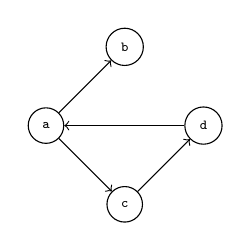
\begin{tikzpicture}
\node[draw, circle] (b) at (0, 0) {\tiny \texttt{b}};
\node[draw, circle] (a) at (-1, -1) {\tiny \texttt{a}};
\node[draw, circle] (d) at (1, -1) {\tiny \texttt{d}};
\node[draw, circle] (c) at (0, -2) {\tiny \texttt{c}};
\draw[->] (a) -- (b);
\draw[->] (a) -- (c);
\draw[->] (c) -- (d);
\draw[->] (d) -- (a);
\end{tikzpicture}
\end{center}
est repr\'{e}sent\'{e} par: \\

\noindent \texttt{link(a, b)}. \\
\texttt{link(a, c)}. \\
\texttt{link(c, d)}. \\
\texttt{link(d, a)}.

\begin{enumerate}
 \item \'{E}crivez un pr\'{e}dicat \texttt{path(X, Y)} qui est vrai s'il exsite un chemin de X \`{a} Y.
 \item Est-ce que l'ordre des pr\'{e}dicats dans votre programme a de l'importance?
 \item Comment calculer le chemin, et pas juste savoir s'il y en a un? Vous pouvez calculer le
 chemin dans l'ordre inverse si c'est plus simple.
 \item Comment on fait pour calculer tous les chemins entre X et Y?
\end{enumerate}

    \subsubsection*{Solution}
    \begin{enumerate}
    \item \textbf{TODO}
    \item \textbf{TODO}
    \item
    \begin{lstlisting}

    /* Partie 1 : Existence */

    link(a, b).
    link(a, c).
    link(c, d).
    link(d, a).

    path(X, Y) :- link(X, Y).
    path(X, Y) :- link(X, Z), path(Z, Y).

    /* Partie 2 : Ordre *

    path(X,Y) :- path(Z, Y), link(X, Z).
    %*\text{\% Fonctionne aussi, mais moins efficace.}*)
    %*\text{\% L’ordre des predicats n’a de l’importance que pour les performances.} *)

    /* Partie 3 : Chemin */

    link(a, b, [a, b]).
    link(a, c, [a, c]).
    link(c, d, [c, d]).

    path(X, Z, P) :- link(X, Z, P).
    path(X, Z, [X|P2]) :- link(X, Y, P1), path(Y, Z, P2).
    \end{lstlisting}

    \item Pour calculer tous les chemins, il suffit de lancer le programme de la partie 3, puis d'attendre une réponse.
    Lorsqu'on a une solution, on peut demander au programme de revenir en arrière et de modifier son dernier choix pour trouver une solution différente.
    En pratique, cela peut se faire en répondant à la réponse du programme par un ";" au lieu d'un ".".
    Il n'y a qu'à réitérer l'opération jusqu'à ce que le programme n'ait plus de choix disponible et qu'il se termine pour de bon.

   \end{enumerate}
\subsection*{Exercice 6}
Le programme suivant d\'{e}cide si un nombre est premier ou pas.

\begin{verbatim}
isPrime(2).
isPrime(3).
isPrime(P) :- P > 3, P mod 2 =\= 0, \+ hasFactor(P,3).
hasFactor(N,L) :- N mod L =:= 0.
hasFactor(N,L) :- L * L < N, L2 is L + 2, hasFactor(N,L2).
\end{verbatim}
Montrez les \'{e}tapes que prolog fait pour r\'{e}pondre aux requ\^{e}tes \texttt{isPrime(15)} et \texttt{isPrime(17)}.

    \subsubsection*{Solution}

    \begin{lstlisting}
    /* Requête initiale */
    r0 = < isPrime(15). >


    /* Résolution 1 */
    s1 = {(P, 15)}        % On sait que la variable P
                          % de la fonction isPrime vaut 15
    r1 = < 15>3, 15 mod 2 =\= 0, \+ hasFactor(15, 3). >
    % On developpe la fonction isPrime

    /* Résolution 2 */
    s2 = s1
    r2 = < 15 mod 2 =\= 0, \+ hasFactor(15, 3). >
    %15 est bien strictement superieur a 3

    /* Résolution 3 */
    s3 = s2
    r3 = < \+ hasFactor(15, 3). >
    %15 n'est pas divisible par 2

    /* Résolution 4 */
    s4 = s3 U {(L, 3)}     %On developpe hasFactor
    r4 = < \+ 3*3 < 15, L2 is 3+2, hasFactor(15, L2). >

    /* Résolution 5 */
    s5 = s4
    r5 = < \+ L2 is 3+2, hasFactor(15, L2). >

    /* Résolution 6 */
    s6 = s5 U {(L2, 5)}
    r6 = < \+ hasFactor(15, 5). >

    /* Résolution 7 */
    s7 = s6
    r7 = < \+ 15 mod 5 =:= 0. >
    %On passe dans le cas de base

    /* Résolution 8 */
    s8 = s7
    r8 = < \+ true >

    %La resolvante s'arrete car on a \+ true
    %(\+ implique que ce qui suit doit etre false)
    \end{lstlisting}

    \begin{lstlisting}
    /* Requête initiale */
    r0 = < isPrime(17). >


    /* Résolution 1 */
    s1 = {(P, 17)}        % Meme debut
    r1 = < 17>3, 17 mod 2 =\= 0, \+ hasFactor(17, 3). >

    /* Résolution 2 */
    s2 = s1
    r2 = < 17 mod 2 =\= 0, \+ hasFactor(17, 3). >

    /* Résolution 3 */
    s3 = s2
    r3 = < \+ hasFactor(17, 3). >

    /* Résolution 4 */
    s4 = s3 U {(L, 3)}     %On developpe hasFactor
    r4 = < \+ 3*3 < 17, L2 is 3+2, hasFactor(17, L2). >

    /* Résolution 5 */
    s5 = s4
    r5 = < \+ L2 is 3+2, hasFactor(17, L2). >

    /* Résolution 6 */
    s6 = s5 U {(L2, 5)}
    r6 = < \+ hasFactor(17, 5). >

    /* Résolution 7 */
    s7 = s6
    r7 = < \+ 5*5 < 17, L2' is 5+2, hasFactor(17, L2'). >
    %25 n'est pas inferieur a 17; false

    /* Résolution 8 */
    s8 = s7
    r8 = < \+ false >

    /* Résolution 9 */
    s9 = s8
    r9 = < >
    %La resolvante est vide
    %La requete renvoie true
    \end{lstlisting}


\section{TP 9}


\subsection*{Exercice 1}
Soient $x, y$ et $z$ trois n\oe{}uds distincts. On dit que $x$ est un \emph{n\oe{}ud pivot} pour $y$ et $z$ si tous les chemins les plus courts entre $y$ et $z$ passent par $x$.

\begin{enumerate}
\item Donnez un exemple d'un graphe o\`{u} tous les n\oe{}uds sont un n\oe{}ud pivot pour au moins une paire de n\oe{}uds.
\item Donnez un exemple d'un graphe o\`{u} tous les n\oe{}uds sont un n\oe{}ud pivot pour au moins trois paires de n\oe{}uds.
\item Soit $G$ un graphe qui repr\'{e}sente les liens d'amiti\'{e} d'un groupe de personnes. Si on suppose que la probabilit\'{e}e que deux personnes qui ne sont pas amies au
temps $t$ deviennent amies au temps $t + 1$ est inversement proportionelle a la distance entre elles, quel est l'effet sur la probabilit\'{e} de retirer un personne pivot du graphe?
\item Montrez qui si tous les n\oe{}uds sont un n\oe{}ud pivot pour au moins une paire de n\oe{}uds alors le graphe poss\'{e}de au moins un cycle.
\end{enumerate}

\subsubsection*{Solution}

\begin{enumerate}
	\item On prend $G = $
\begin{center}
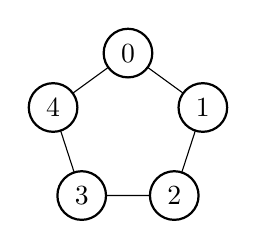
\begin{tikzpicture}
\tikzstyle{node}=[circle,draw,thick,fill=white]
\draw (90:1) node[node]{0}
-- (162:1) node[node]{4}
-- (234:1) node[node]{3}
-- (306:1) node[node]{2}
-- (378:1) node[node]{1}
-- cycle;
\end{tikzpicture}
\end{center}
$\forall i$ le noeud $i$ est pivot de $(i-1)\&(i+1)$ (modulo 5).

	\item On prend $G = $
\begin{center}
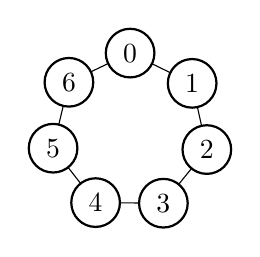
\begin{tikzpicture}
\tikzstyle{node}=[circle,draw,thick,fill=white]
\draw (90:1) node[node]{0}
-- (141:1) node[node]{6}
-- (192:1) node[node]{5}
-- (244:1) node[node]{4}
-- (295:1) node[node]{3}
-- (347:1) node[node]{2}
-- (398:1) node[node]{1}
-- cycle;
\end{tikzpicture}
\end{center}

$\forall i$ le noeud $i$ est pivot de :
$(i-1) \& (i+1)$, $(i-1) \& (i+2)$ et $(i-2) \& (i+1)$
(modulo 7).
	\item Retirer le noeud pivot augmente la distance entre 2 personnes. Donc la probabilité que celles ci deviennent amies au temps $t+1$ diminue.

	\item On prouve d'abord que si un graphe n'a pas de cycle alors il possède au moins un noeud de degré 1.

Supposons que $G$ n'a pas de cycle et $V$ l'ensemble fini de ses noeuds.
Soit $x \in V$. On construit une séquence $P = (x_1, x_2, x_3, ...)$. Pour choisir $x_i (i>1)$, on prend un voisin de $x_{i-1}$ qiu n'a pas encore été choisi. Comme $V$ est fini, ce processus doit finir et on obtient $P= (x_1, x_2, x_3,...,x_k)$.
Le noeud $k$ a un degré 1 car sinon il a un voisin $y\neq x_{k-1}$. Si $y \in P$ : Contradiction.
Si $y \notin P$, $x_k$ n'est pas la fin de la séquance : Contradiction.

On prouve ensuite que un noeud de degré un ne peu pas etre pivot.

Soit $x\in V$ tel que deg$(x)=1$.
Par hypothèse $x$ est pivot d'une paire $(y,z)$.
Donc il existe un chemin le plus court entre $y$ et $z$ qui passe bien par $x$.
Soit $w$ le seul voisin de $x$.
Mais alors il existe un chemin encore plus court : $(y, ..., w,...,z)$ qui ne passe pas par $x$.

% Insérer graphe

\end{enumerate}
\subsection*{Exercice 2}
Soient $x, y$ et $z$ trois n\oe{}uds distincts. On dit que $x$ est un \emph{gardien} de $y$ et $z$ si tous les chemins entre $y$ et $z$ passent par $x$.
On dit qu'un n\oe{}ud $x$ est un \emph{gardien locale} s'il existent deux voisins de $x$ qui ne sont pas connect\'{e}s directement.

\begin{enumerate}
\item Donnez un exemple d'un graphe o\`{u} au moins la moiti\'{e} des n\oe{}uds sont
gardiens.
\item Donnez un exemple d'un graphe o\`{u} il n'y a pas de gardiens mais chaque n\oe{}ud est un gardien locale.
\item Quel est l'impacte sur un graphe de retirer un gardien?
\end{enumerate}

\subsubsection*{Solution}
\begin{enumerate}
	\item Les noeuds 1 et 2 sont gardien entre 0 et 3

\begin{center}
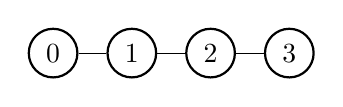
\begin{tikzpicture}
    \tikzstyle{node}=[circle,draw,thick,fill=white]
    \node[node] (0) at (0,0) {0};
    \node[node] (1) at (1,0) {1};
    \node[node] (2) at (2,0) {2};
    \node[node] (3) at (3,0) {3};

    \draw (0) -- (1);
    \draw (1) -- (2);
    \draw (2) -- (3);
\end{tikzpicture}
\end{center}

	\item  \hspace{1em}
	\vspace{1em}

\begin{center}
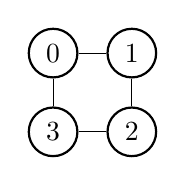
\begin{tikzpicture}
\tikzstyle{node}=[circle,draw,thick,fill=white]
    \node[node] (0) at (0,0) {0};
    \node[node] (1) at (1,0) {1};
    \node[node] (2) at (1,-1) {2};
    \node[node] (3) at (0,-1) {3};

    \draw (0) -- (1);
    \draw (1) -- (2);
    \draw (2) -- (3);
    \draw (3) -- (0);
\end{tikzpicture}
\end{center}

	\item Le graphe n'est plus connexe
\end{enumerate}

\subsection*{Exercice 3}

\begin{enumerate}
 \item Comment peut-on faire pour calculer efficacement les distances d'un n\oe{}uds a tout les autres?
 \item Un graphe est biparti si on peut s\'{e}parer les n\oe{}uds en deux ensembles $V_1$ et $V_2$ tells que
 $V_1 \cap V_2 = \emptyset$, $V_1 \cup V_2 = V$ et il n'y a pas d'ar\^{e}tes entre aucune paire de n\oe{}uds de $V_1$ et
 pas d'ar\^{e}tes entre aucune paire de n\oe{}uds de $V_2$. Soit $G$ un graphe connexe et $d_0(x)$ la distance du n\oe{}ud
 $0$ au n\oe{}ud $x$. Comment peut-on v\'{e}rifier que $G$ est bipartit a partir de $d_0$?
\end{enumerate}

\subsubsection*{Solution}
\begin{enumerate}

	\item On utilise l'algorithme BFS qui utilise une \texttt{Queue FIFO}
\begin{enumerate}
    \item Mettre le n\oe{}ud dans la Queue.
    \item Retirer le n\oe{}ud du début de la Queue pour l'examiner.
    \item Mettre tous les voisins non explorés dans la Queue.
    \item Si la file n'est pas vide reprendre à l'étape 2.
\end{enumerate}

Exemple :

\begin{tabular}{lll}
    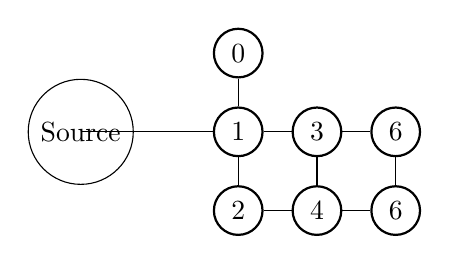
\begin{tikzpicture}
    \tikzstyle{node}=[circle,draw,thick,fill=white]
    \node[node] (2) at (0,0) {2};
    \node[node] (1) at (0,1) {1};
    \node[node] (0) at (0,2) {0};
    \node[node] (4) at (1,0) {4};
    \node[node] (3) at (1,1) {3};
    \node[node] (5) at (2,1) {6};
    \node[node] (6) at (2,0) {6};
    \node[] (S) at (-2,1) {Source};

    \draw (S) |- (1.west);
    \draw (0) -- (1);
    \draw (1) -- (2);
    \draw (3) -- (1);
    \draw (2) -- (4);
    \draw (4) -- (3);
    \draw (3) -- (5);
    \draw (6) -- (4);
    \draw (5) -- (6);
\end{tikzpicture}
&

&
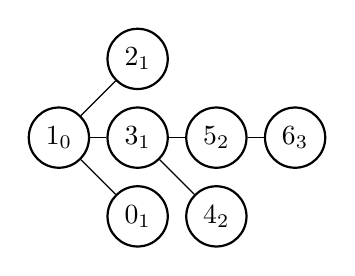
\begin{tikzpicture}
    \tikzstyle{node}=[circle,draw,thick,fill=white]
    \node[node] (1) at (0,1) {$1_{0}$};
    \node[node] (0) at (1,0) {$0_{1}$};
    \node[node] (3) at (1,1) {$3_{1}$};
    \node[node] (2) at (1,2) {$2_{1}$};
    \node[node] (5) at (2,1) {$5_{2}$};
    \node[node] (4) at (2,0) {$4_{2}$};
    \node[node] (6) at (3,1) {$6_{3}$};

    \draw (1) -- (0);
    \draw (1) -- (3);
    \draw (1) -- (2);
    \draw (3) -- (5);
    \draw (3) -- (4);
    \draw (5) -- (6);
\end{tikzpicture}
\end{tabular}

\item On vérifie qu'il n'existe pas d'arètes $(x,y)$ tel que $d_0(x)$ et $d_0(y)$ ont la meme parité

\end{enumerate}

% \vspace{0.5cm}
%
% \subsection*{Exercice }
% Soient $x, y$ et $z$ trois n\oe{}uds distincts. On dit que $x$ est un \emph{gardien} de $y$ et $z$ si tous les chemins entre $y$ et $z$ passent par $x$.
% On dit qu'un n\oe{}ud $x$ est un \emph{gardien locale} s'il existent deux voisins de $x$ qui ne sont pas connect\'{e}s directement.
%
% \begin{enumerate}
% \item Donnez un exemple d'un graphe o\`{u} au moins la moiti\'{e} des n\oe{}uds sont
% gardiens.
% \item Donnez un exemple d'un graphe o\`{u} il n'y a pas de gardiens mais chaque n\oe{}ud est un gardien locale.
% \end{enumerate}
%

\subsection*{Exercice 4}
Le \emph{diam\`{e}tre} d'un graphe connexe est la distance maximum entre toutes les paires de n\oe{}uds.
La \emph{distance moyenne} d'un graphe connexe c'est la moyenne des distances entre toutes les paires de n\oe{}uds. Formellement
$$
diam(G) = \max_{u, v} d(u, v)
$$
et
$$
l_G = \frac{1}{V (V - 1)} \sum_{u \neq v} d(u, v)
$$
o\'{u} $V$ est le nombre de n\oe{}uds de $G$.
\begin{enumerate}
\item Calculez le diam\`{e}tre et la distance moyenne du graphe $G_n$ suivant:
\begin{center}
\begin{tikzpicture}
\node[draw, circle] (A) at (0, 0) {0};
\node[draw, circle] (B) at (2, 0) {1};
\node[draw, circle] (C) at (4, 0) {2};
\node[draw, circle] (D) at (6, 0) {3};
\draw (A) -- (B) -- (C) -- (D);
\draw[dashed] (7, 0) circle (2);
\node at (9.5, 1) {$K_n$};
\draw (D) -- (7, 1);
\node at (7, 0.4) {$\vdots$};
\draw (D) -- (7, -0.5);
\draw (D) -- (7, -1);
\end{tikzpicture}
\end{center}
o\`{u} $K_n$ est le graphe complet avec $n$ n\oe{}uds. Par example, $G_4$ est le graphe:
\begin{center}
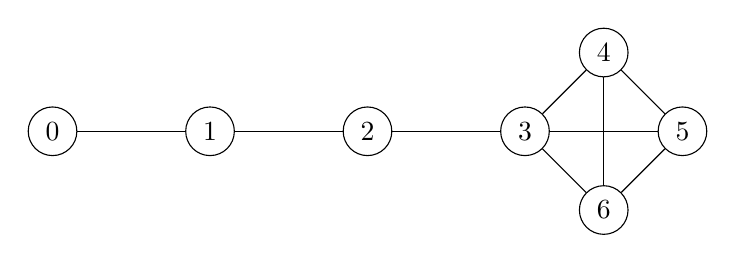
\begin{tikzpicture}
\node[draw, circle] (A) at (0, 0) {0};
\node[draw, circle] (B) at (2, 0) {1};
\node[draw, circle] (C) at (4, 0) {2};
\node[draw, circle] (D) at (6, 0) {3};
\node[draw, circle] (E) at (7, 1) {4};
\node[draw, circle] (F) at (8, 0) {5};
\node[draw, circle] (G) at (7, -1) {6};

\draw (A) -- (B) -- (C) -- (D);
\draw (D) -- (E);
\draw (D) -- (F);
\draw (D) -- (G);
\draw (E) -- (F);
\draw (E) -- (G);
\draw (G) -- (F);
\end{tikzpicture}
\end{center}


\item Montrez qu'il existe un graphe $G$ avec plus de $7$ n\oe{}uds tel que
$$\frac{diam(G)}{l_G} = 2$$

\end{enumerate}


% \subsection*{Exercice }
% Calculez le coefficient regroupement de A et de B dans le graphe suivant:
% \begin{center}
% \begin{tikzpicture}
% \node[draw, circle] (A) at (0, 0)   {A};
% \node[draw, circle] (B) at (-2, 1)  {B};
% \node[draw, circle] (C) at (2, 1)   {C};
% \node[draw, circle] (D) at (2, -1)  {D};
% \node[draw, circle] (E) at (-2, -1) {E};
% \node[draw, circle] (F) at (-4, 0)  {F};
% \draw (A) -- (B);
% \draw (A) -- (C) -- (D);
% \draw (A) -- (D);
% \draw (A) -- (E) -- (B);
% \draw (B) -- (F) -- (E);
% \end{tikzpicture}
% \end{center}
%
%
% \vspace{0.5cm}

\subsubsection*{Solution}
\begin{enumerate}

	\item dim$(G) = 4$

Selon la table des distance:

\begin{tabular}{c|ccccc}
    &0&1&2&3& >3 \\
    \hline
    0 & 0& 1& 2& 3& 4\\
    1 & 1& 0&1& 2& 3\\
    2 & 2& 1& 0& 1&2\\
    3 & 1& 2& 3& 0&1\\
    >3 & 4& 3& 2& 1& 1 (0 si lui meme)\\
\end{tabular}

On peut calculer $\sum_{u\neq v} d(u,v)$.

\begin{align*}
    \sum_{u\neq v} d(u,v) =& 6 + 4(n-1)\\
    &+ 4 + 3(n-1)\\
    &+4+2(n-1)\\
    &+6+(n-1)\\
    &+(n-1)(10 + (n-2))\\
    =& 20 + (n-1)(4+3+2+1) + (n-1)(9 + (n-2))\\
    =& 20 + 10(n-1) + 9(n-1) + (n-1)^2\\
    =& 20 + 19(n-1) + (n-1)^2\\
    & \Rightarrow l_G (n) = \dfrac{n^2 + 17n + 2}{n^2 + 5n + 6}
\end{align*}


	\item $\dfrac{\text{diam}(G)}{l_G} = \dfrac{4}{l_G} =2$
\begin{align*}
    & \dfrac{4n^2 + 20n + 24}{n^2 + 17n + 2} = 2\\
    & \Rightarrow 4n^2 + 20n + 24 = 2n^2 + 34n + 4\\
    & \Rightarrow 2n^2 - 14n + 2\\
    & \Rightarrow n = 5\hspace{1em}\&\hspace{1em} n = 2\\
\end{align*}

Or $G$ doit comporter au moins 7 noeuds donc $G(5)$.

\end{enumerate}

\subsection*{Exercice 5}
On suppose qu'on est dans une communaut\'{e} ou les amiti\'{e}s sont repr\'{e}sent\'{e}es par un graphe $G$ connexe avec $n$ n\oe{}uds.
Si chaque jour les amis des amis se rencontrent et deviennent amis, on s'interesse au nombre de jours $T(G)$ n\'{e}cessaires
pour que tout le monde deviennent ami, c'est-\`{a}-dire, pour le graphe deviennent $K_n$ (un graphe complet).
\begin{enumerate}
\item Supposons que $G = P_n$ (le chemin avec $n$ n\oe{}uds) et $T(P_n)$.
\item M\^{e}me question pour $G = C_n$ (le cycle avec $n$ n\oe{}uds).
\item Quel est la valeur de $T(G)$ en g\'{e}neral?
\end{enumerate}

\subsubsection*{Solution}
\begin{enumerate}

	\item Soit $A(i)$, les amis de $0$ au jour $i$.
\begin{align*}
    A(0) =& \{1 \} \\
    A(1) =& \{1,2 \}\\
    A(2) =& \{1,2,3,4 \}\\
    A(3) =& \{1,2,3,4,5,6,7,8, \}\\
    A(i) =& \{x+y | x,y \in A(i-1) \} \\
         =& \{1,2,3,..., 2^i \} \\
    T(P_n) =& \lceil \log_2 (n) \rceil
\end{align*}


	\item Le noeud le plus loin de $0$ dans un cycle de $n$ noeuds, est le noeud $\left\lfloor \dfrac{n}{2} \right\rfloor$
$$ T(C_n) = \left\lceil \log_2 \left(\left\lfloor \dfrac{n}{2} \right\rfloor \right) \right\rceil $$

	\item En général les noeuds à distance maximum prennent le plus de temps. Cette distance est le diamètre du graphe. Donc :
$$ T(G) = \left\lceil \log_2 \left( \text{dim}(G) \right) \right\rceil $$


\end{enumerate}
%
% \subsection*{Exercice }
% Calculez le coefficient de regroupement d'un n\oe{}ud de $C_n$, o\`{u} $n \geq 3$. Calculez le coefficient de regroupement de ce n\oe{}ud ap\`{e}s avoir ajout\'{e} les ar\^{e}tes entre les amis des amis dans le graphe. Commentez.
%
%
%
% \subsection*{Exercice }
% \'{E}noncez la propri\'{e}t\'{e} de fermeture triadique forte. Est-ce que le graphe suivant poss\`{e}de cette propri\'{e}t\'{e}?
%
% \begin{center}
% \begin{tikzpicture}
% \node[draw, circle] (A) at (0, 0) {A};
% \node[draw, circle] (B) at (2, 0) {B};
% \node[draw, circle] (C) at (0, -2) {C};
% \node[draw, circle] (D) at (-2, 0) {D};
% \node[draw, circle] (E) at (0, -4) {E};
% \node[draw, circle] (F) at (2, -2) {F};
% \node[draw, circle] (G) at (-2, -4) {G};
% \draw (G) -- (D) -- (A) -- (C) -- (F);
% \draw (C) -- (E);
% \draw[dashed] (G) -- (A) -- (B) -- (F) -- (E) -- (G);
% \draw[dashed] (D) -- (C);
%
% \draw (4, -1) -- (5, -1) node[anchor = west] {lien fort};
% \draw[dashed] (4, -2) -- (5, -2) node[anchor = west] {lien faible};
% \end{tikzpicture}
% \end{center}
%
% Supposons qu'un graphe poss\`{e}de la propri\'{e}t\'{e} de fermeture triadique forte. Si un lien faible devient fort, est-ce que cette propri\'{e}t\'{e} se maintien toujours? Et si un lien fort devient faible?
%
%


\section{}

% From TP4
\subsection{Exercise 1 (Authenticated encryption, or not; August Exam)}

Let $\Pi \define \langle \Gen, \Enc, \Dec\rangle$ be an authenticated encryption
scheme such that $\Enc$ encrypts messages of $n$ bits.
%
Do the following systems provide authenticated encryption?  For those
that do, briefly explain why.  For those that do not, present an
attack that breaks one of the security properties of an authenticated
encryption scheme.

\begin{enumerate}
	\item $\Pi' \define \langle \Gen, \Enc', \Dec'\rangle$ with
	$\Enc'_k(m) = (\Enc_k(m), \Enc_k(m \oplus (0^{n-1}\|1)))$ and
	$\Dec'_k(c_1, c_2) = \Dec_k(c_1)$ if
	$\Dec_k(c_1) \oplus \Dec_k(c_2) = 0^{n-1}\|1$ and $\bot$ otherwise.

	\item $\Pi' \define \langle \Gen, \Enc', \Dec'\rangle$ with
	$\Enc'_k(m) = (\Enc_k(m), \Mac_k(m))$ and $\Dec'_k(c_1, c_2) = \Dec_k(c_1)$

	if $\Vrfy_k(\Dec_k(c_1), c_2)=1$ and $\bot$ otherwise. Here, $\Mac$
	and $\Vrfy$ are deterministic algorithms that are part of a secure
	MAC scheme that is compatible with $\Gen$.
\end{enumerate}

\begin{solution}
	$\Pi \define \langle \text{Gen, Enc, Dec} \rangle$ is an authenticated encryption scheme (AE) if it is CCA-secure and unforgeable.
	\begin{enumerate}
		\item The system $\Pi'$ is not AE because it is \textbf{forgeable} and we can show it with this example. If the adversary A asks for the message $m$ ($m'$ corresponds to the message m with the last bit changed) to the oracle access, he will receive the cipher text $(c_1, c_2)$, where $c_1 = \Enc_k(m)$ and $c_2 = \Enc_k(m\xor 0^{n-1}||1) = \Enc_k(m')$.

		If $\A$ outputs the pair (m',$(c_2, c_1)$), this is a forgery.

		$\Dec_k'(c_2,c_1) = \Dec_k(c_2) = \Dec_k(\Enc_k(m')) = m' \neq \bot $ because $\Dec_k(c_2) \oplus \Dec_k(c_1) = m' \oplus m = m \oplus 0^{n-1}||1 \oplus m = 0^{n-1}||1 $.
		And $m'$ has not been requested before.

		Then we have EncForge$_{A, \Pi'}$(n) = 1  and Pr[EncForge$_{A, \Pi'}$(n)] = 1. $\Pi'$ is then forgeable and it is not an AE.

		With the same technique, an adversary can break the CCA-security of this scheme by querying two different messages $m_1$ and $m_2$, obtaining their encryption, sending \newline
		($m'_1,m'_2$) = ($m_1 \oplus 0^{n-1}||1, m_2 \oplus 0^{n-1}||1$) for the challenge, and compare the encryption of $m'_b$ with the two previously received ciphertexts.

		Note that this doesn't break CPA-security; indeed, the scheme is still CPA-secure.

		\item The sytem $\Pi'$ is not AE because it is not \textbf{CCA-secure} and we can show it because $Mac_k(m)$ does not assure any security (only authentication). So if We use as Mac:
		\[ \Mac_k(m) = m||\Mac'_k(m) \]
		It is a good mac but it is trivial to show that it is not CCA-Secure. $\Pi'$ is then not an AE.

		\strong{Stronger argument}:

		The adversary can send two different messages $m_0$ and $m_1$ to the encryption oracle to get $(\Enc_k(m_0), \Mac_k(m_0))$ and $(\Enc_k(m_1), \Mac_k(m_1))$.

		We then output the same $m_0$ and $m_1$, and receive $(\Enc_k(m_b), \Mac_k(m_b))$.

		As $\Pi$ is an athenticated encryption scheme, we know that $\Enc$ is probabilistic and secure.
		However, $\MAC$ is said to be deterministic, and this causes $\Mac_k(m_b)$ to be the same as one of the $\Mac_k(m_0)$, $\Mac_k(m_1)$ received earlier.
		We can thus just compare the tags, and output the corresponding $b'$.

		The probability of success is $\Pr[b'=b] = \Pr[\Mac_k(m0) \neq \Mac_k(m_1)]=1-\negl(n)$ which is clearly well above what it should be.
	\end{enumerate}
\end{solution}



\subsection{Exercise 2 (Derandomizing signatures)}

Let $S=(\Gen, \Sign, \Vrfy)$ be an EUF-CMA signature scheme defined over $(M, \Sigma)$, where the signing algorithm $\Sign$ is probabilistic.
In particular, algorithm $\Sign$ uses randomness chosen from a space $R$.
We let $\mathsf{S}(sk, m; r)$ denote the execution of algorithm $\mathsf{S}$ with randomness $r$.
Let $F$ be a secure PRF defined over $(K, M, R)$.
Show that the following signature scheme with deterministic signing $S'=(\Gen', \Sign', \Vrfy)$ is EUF-CMA:
\[ \mathsf{G}'(1^n) \define \left\{ (pk, sk) \pick \G(1^n), \qquad k \pick K, \qquad sk' \define (sk, k), \qquad \text{output } (pk, sk') \right\}; \]
\[ \Sign'((sk, k), m) \define \left\{ r \pick F_k(m), \qquad \sigma \pick \mathsf{S}(sk, m; r), \qquad \text{output } \sigma \right\}. \]

\emph{(Hint: Define $S''$ which is like $S'$ byt uses a perfect random function. Make a reduction of the security of $S''$ to the security of $S$, then build a PRF distinguisher based on a adversary against the signature. Finally, compute the link of the advantages of three relevant games.)}


\begin{solution}
	We will prove this in two steps.
	\begin{itemize}
		\item The first step defines $S''$ so that the PRF is replaced by a true random function.
		We will show that in this case, if $S$ is secure, then $S''$ is secure.
		\item The second step proves by reduction that if $S''$ is secure and $F$ is a secure PRF, then $S'$ is secure.
		The reduction proceeds by constructing an adversary $\A_{PRF}$ against the PRF, able to distinguish between the PRF and a random function, given an adversary $\A_{S'}$ against $S'$.
	\end{itemize}

	First, let's define $S''$.
	The only change is that
	\[ \Sign''((sk, k), m) \define \{ r \define f(m), \quad \sigma \define \mathsf{S}''(sk, m), \quad \text{output } \sigma \} \]
	where $\mathsf{S}''(sk, m) = \mathsf{S}(sk, m; f(m))$.

	If we have an adversary against $S''$, we can build an adversary against $S$, simply by relaying oracle calls to $\mathsf{S}_f''(sk, m)$ to our oracle $\mathsf{S}(sk, m; f(m))$.
	As $f$ is a random function, $S$ sees the same randomness as with an $r$, so nothing changes.
	The probabilities are exactly the same:
	\[ \Pr[\Sigforge_{S''}=1] = \Pr[\Sigforge_{S}=1] = \negl(n) \]
	for some $\negl$ negligible.

	Now, let's do the reduction from $F$ to $S'$.
	So, we have an adversary $\A_{S'}$ against $S'$, and we build an adversary against the PRF $\A_F$ as follows:
	\begin{enumerate}
		\item The oracle for the PRF problem $\O_F$ picks $k \pick \K$, kept secret.
		\item $\O_F$ picks $b \pick \bset$, kept secret.
		The oracle defines a challenge function $g=F_k$ if $b=1$, $g=f$ a random function if $b=0$.
		\item $\A_F$ runs $\Gen'$ to create a public key $pk$ and a secret key $sk'=(sk, k)$.
		It discards $k$ as it is not used by $\A_{S'}$ and is defined by $\O_F$.
		It keeps $sk$ secret and sends $pk$ to $\A_{S'}$.
		\item When $\A_{S'}$ asks for $\Sign'((sk, k), m)$, we ask the oracle for $w=g(m)$.
		$w=F_k(m)$ if $b=1$, or $w=f(m)$ with $f$ a random function, if $b=0$.
		We then run $\mathsf{S}(sk, m; r)$ and return the result to $\A_{S'}$.
		\item When $\A_{S'}$ outputs $(m, \sigma)$, its forgery, we outputs $b'=1$ iff $(m, sigma)$ is a valid forgery (we can verify it using $\Vrfy_{pk}$), $b'=0$ otherwise.
	\end{enumerate}
	If $b=0$, we're playing against a true random function, and so we're actually running the scheme $S''$.
	As $\A_{S'}$ is not designed to handle this scheme, its security is the same as the one of $S''$, which is the same as the one of $S$.

	If $b=1$, we're playing the true game for $\A_{S'}$, and so its advantage $\negl'(n)$ is active.

	Then, the difference in probabilities for the distinguishing is:
	\[ |\Pr[\A_F^{F_k}(n)] - \Pr[\A_F^{f}(n)]| = |\negl'(n) - \frac12 \negl(n)| \ge \negl'(n)-\negl(n) \]
	As this difference has to be negligible, as $F$ is a PRF, and $\negl$ is negligible, then $\negl'$ is negligible, and thus the scheme $S'$ is secure.
\end{solution}



\subsection{Exercise 3 (Jan 11 evaluation)}

\copypaste{9}{1}


\section{TP 11}
%\addcontentsline{toc}{section}{TP 11}

% \section*{Rappel}

% Structure du web:

% \begin{center}
% 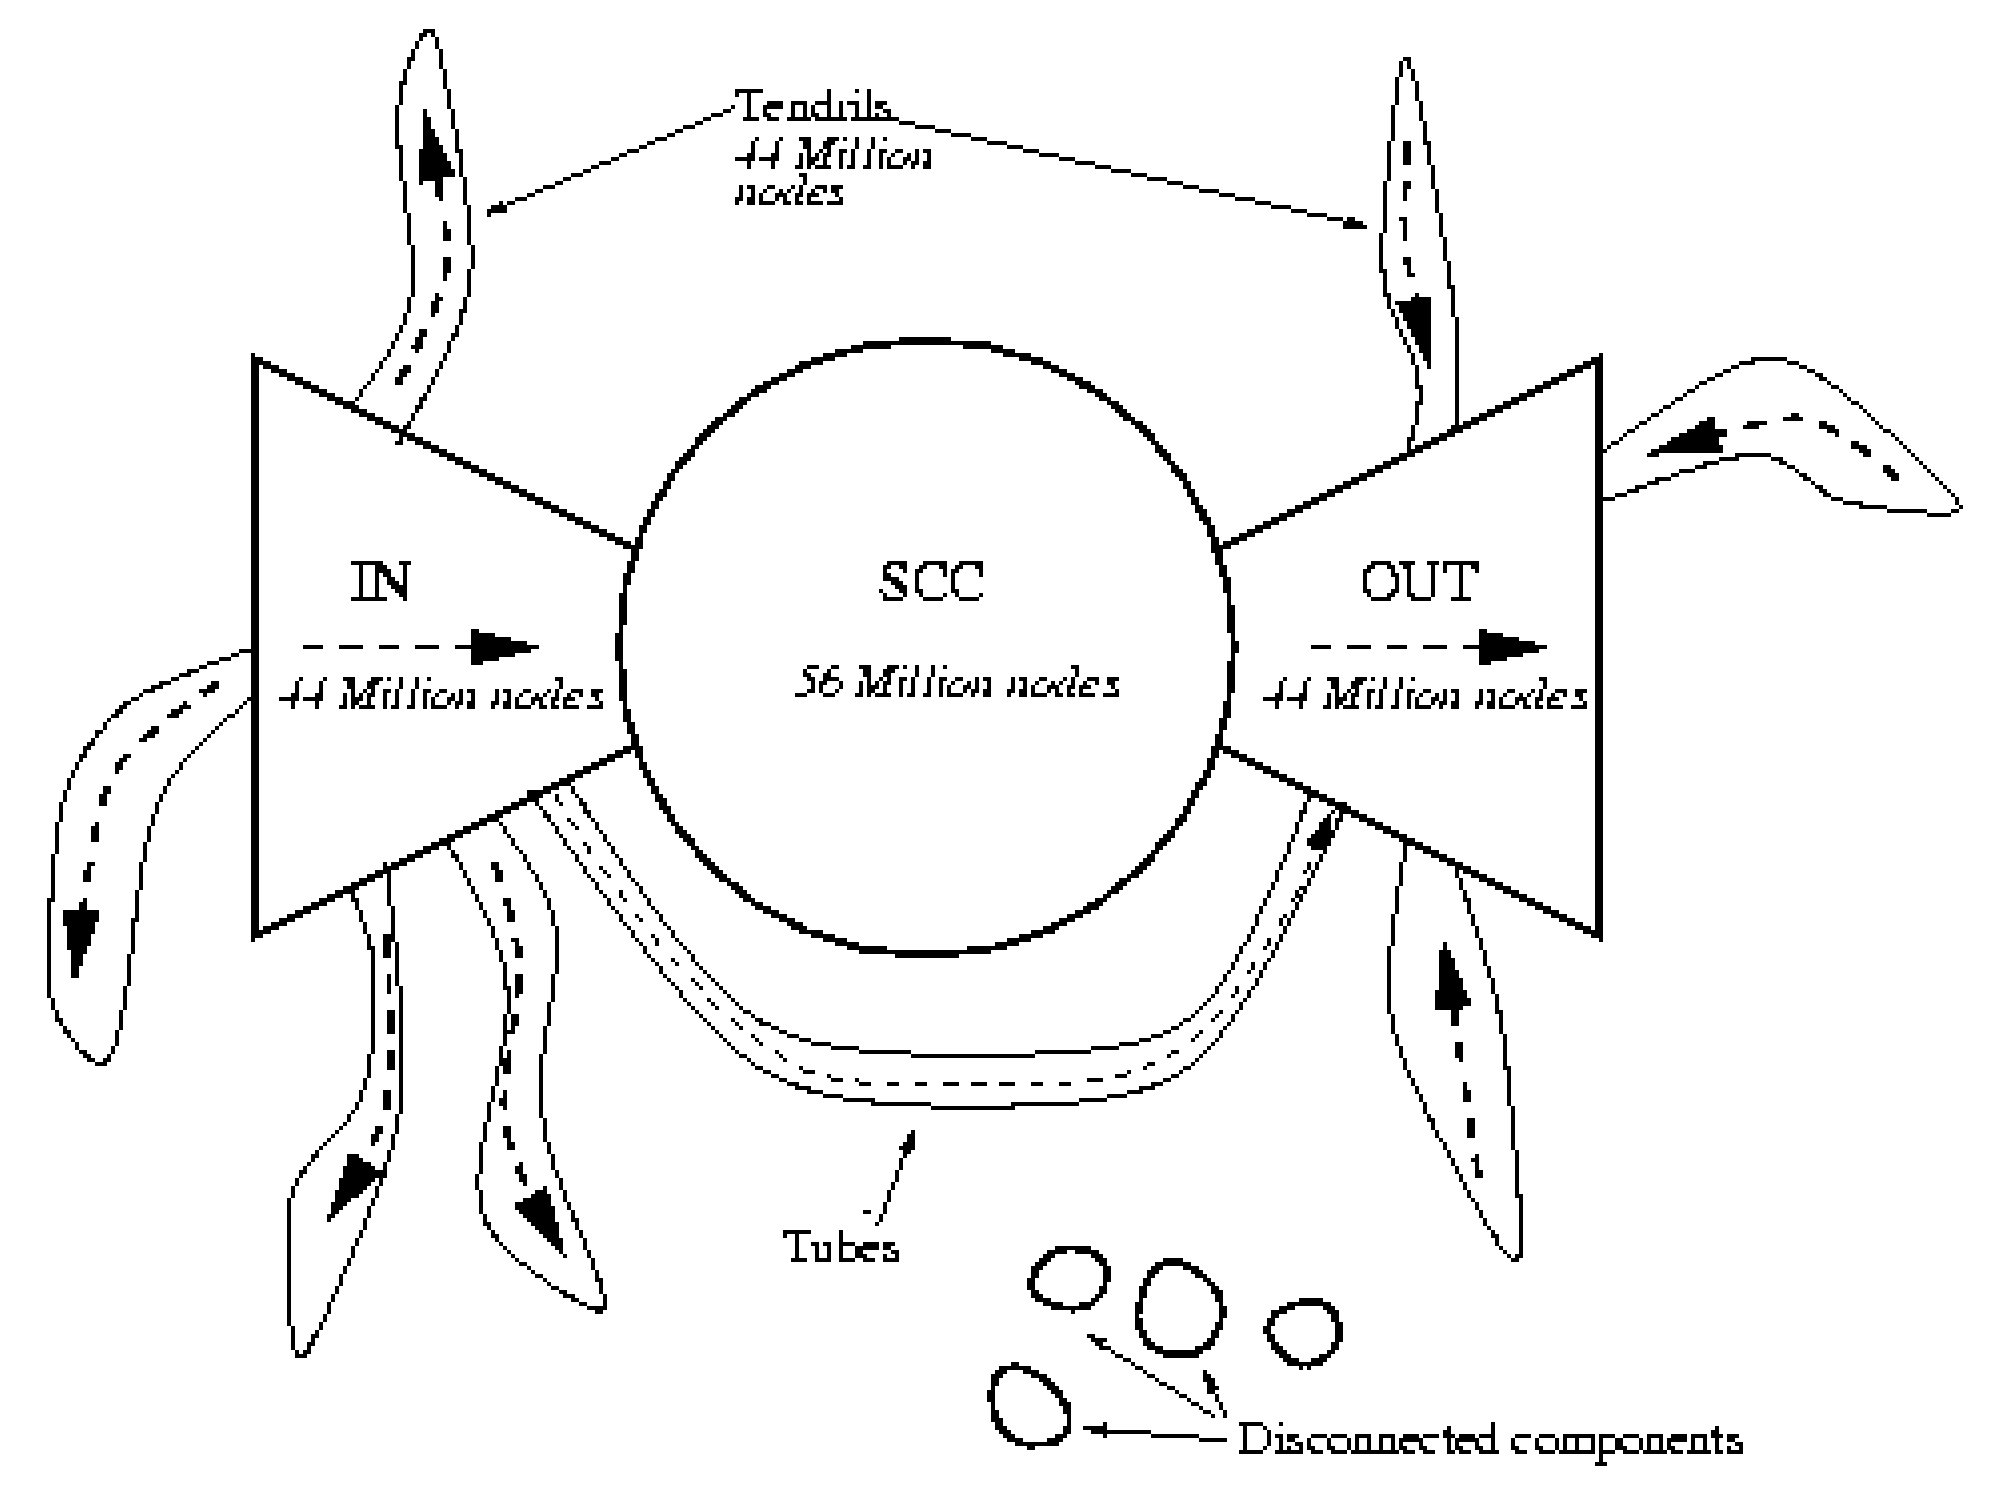
\includegraphics[scale = 0.5]{figs/web.png}
% \end{center}

% On repère trois composants principaux:
% \begin{itemize}
%  \item Un composant \textbf{in}, qui contient des liens hypertextes sortants.
%  \item Un composant fortement connecté principal, qui forme un \textbf{noyau} (SCC).
%  \item Un composant \textbf{out}, qui contient beaucoup de liens hypertextes entrants.
% \end{itemize}


% \newpage

% \section*{Exercices}


\subsection*{Exercice 1}
Considèrer de graphe avec 18 pages Web dans la Figure \ref{fig:webg}. Quels sont les noeuds qui font partie du noyau, les noeuds IN et les noeuds
OUT ? 

    \begin{figure}[h!]
    \begin{center}
    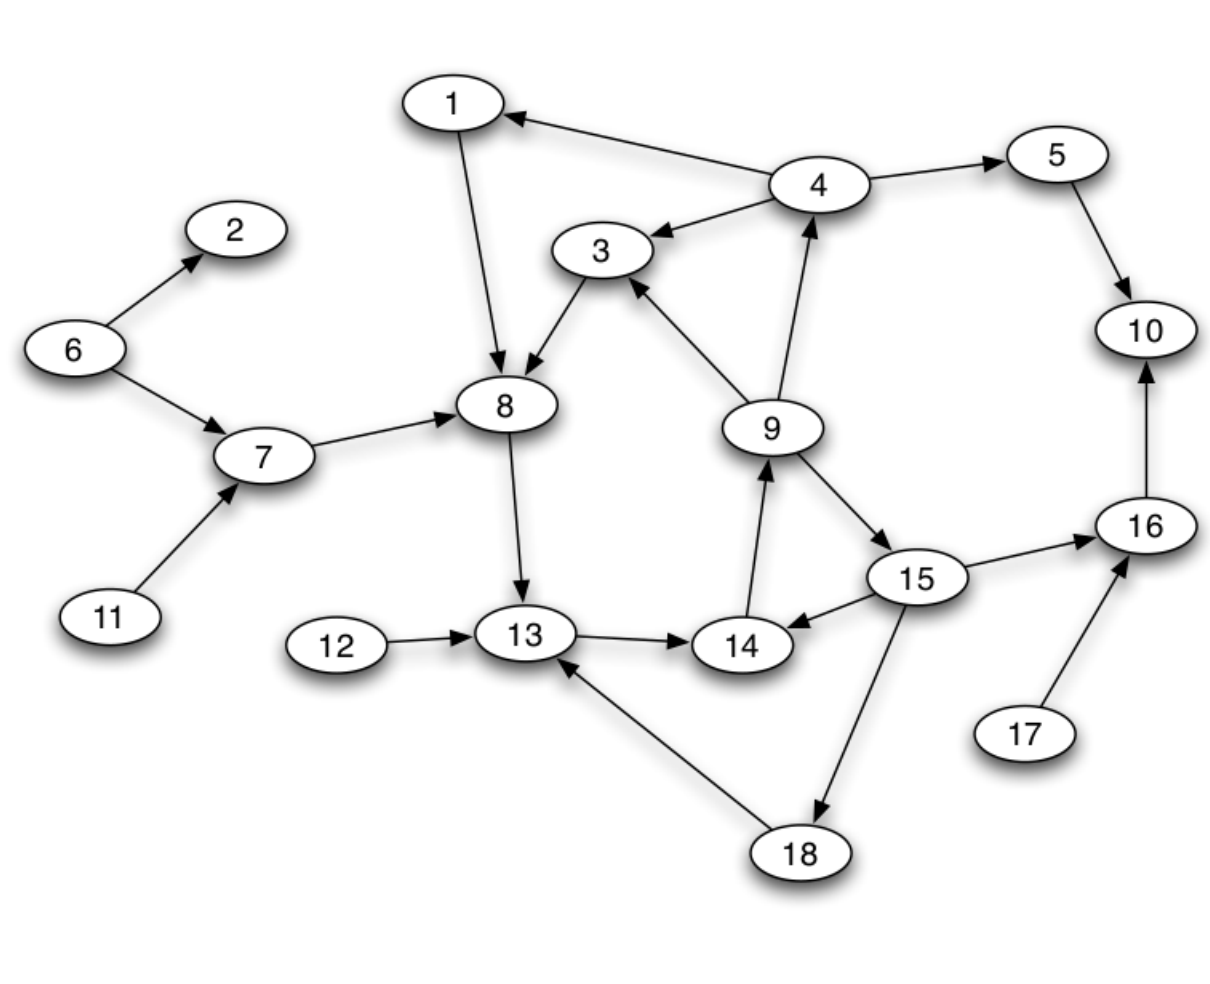
\includegraphics[scale = 0.3]{figs/graph.png}
    \end{center}
    \caption{Un graphe des pages web.}
    \label{fig:webg}
    \end{figure}

    \subsubsection*{Solution}

    \begin{center}
    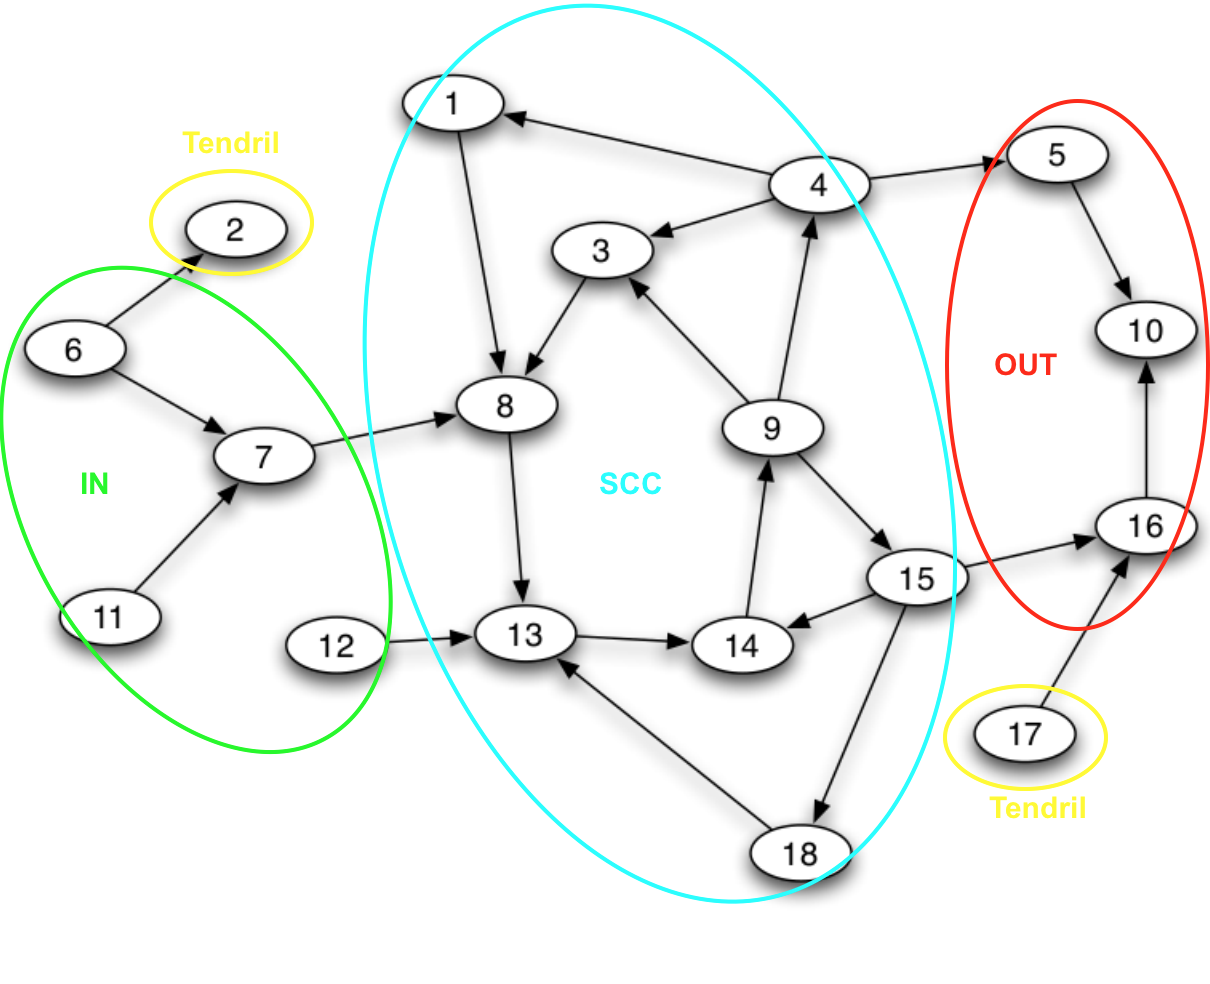
\includegraphics[scale=0.5]{figs/TP11Q1.png}
    \end{center}


\subsection*{Exercice 2}
Pour le graphe de la Figure \ref{fig:webg}.
\begin{enumerate}
 \item Montrez une arête tel que si on l'ajoute ou on la retire, on augmente la taille du noyau.
 \item Montrez une arête tel que si on l'ajoute ou on la retire, on augmente la taille de IN.
 \item Montrez une arête tel que si on l'ajoute ou on la retire, on augmente la taille de OUT.
\end{enumerate}

    \subsubsection*{Solution}

    \begin{center}
    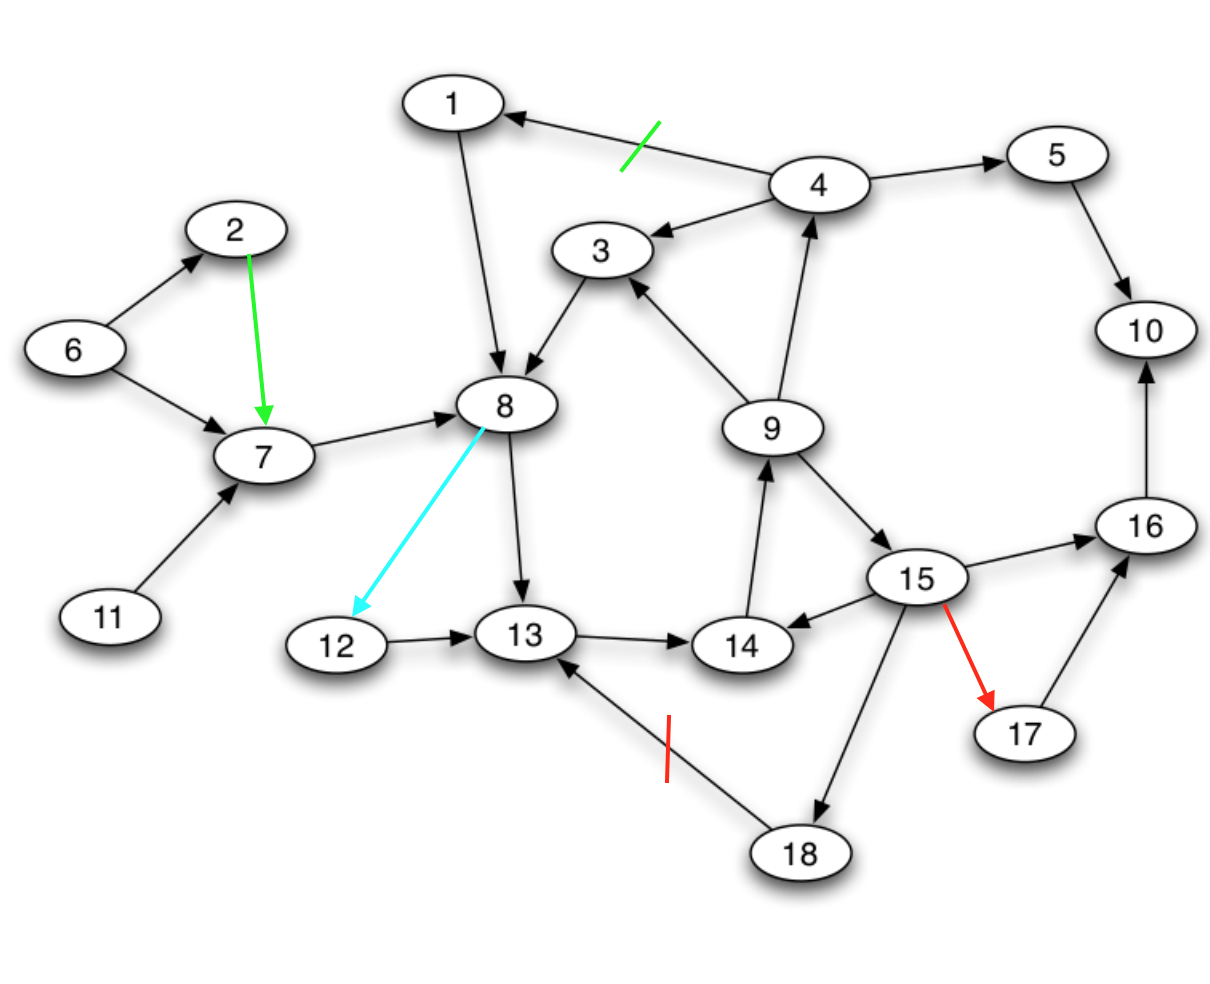
\includegraphics[scale=0.5]{figs/TP11Q2.png}
    \end{center}
    
    \begin{itemize}
        \item Le vert indique une arête à rajouter/retirer pour augmenter la taille du IN.
        \item Le rouge indique une arête à rajouter/retirer pour augmenter la taille du OUT.
        \item Le bleu indique une arête à rajouter pour augmenter la taille du SCC. Il n'est pas possible d'augmenter la taille du SCC en retirant une arête.
    \end{itemize}
    Il y a bien sûr d'autres possibilités que celles-là.


\subsection*{Exercice 3}
Décrivez un graphe tel qu'il existe une arête dont le retrait diminue la taille du noyeau d'au moins 1000 noeuds.

    \subsubsection*{Solution}
    Il faut pour cela un noyau qui possède un ensemble de 1000 noeuds ou plus qui n'est pas relié au IN ni au OUT et qui est relié au reste du noyau par seulement 2 arêtes : une entrante et une sortante.
    Supprimer l'arête qui va de cet ensemble au reste revient à rajouter l'ensemble au IN, tandis que supprimer l'autre arête revient à l'ajouter au OUT.


\subsection*{Exercice 4}
Décrivez un graphe tel qu'il existe une arête dont l'ajout diminue la taille de OUT d'au moins 1000 noueds.

    \subsubsection*{Solution}
    Il faut que le OUT possède une chaîne de 1000 noeuds ou plus et dont au moins un des noeuds de départ est directement lié au noyau.
    Il suffit de rajouter une arête au dernier noeud de cette chaîne pour qu'elle fasse partie intégrante du noyau, et donc pour diminuer la taille de OUT.

\subsection*{Exercice 5}
	\begin{enumerate}
	\item Calculez les valeurs de concentrateurs et d'autorités pour les pages dans le graphe présenté à la Figure \ref{fig:auth} après deux itérations.
	\item Quelles sont les valeurs une fois que la normalisation a été effectuée.
\end{enumerate}

\begin{figure}[!h]
	\centering
	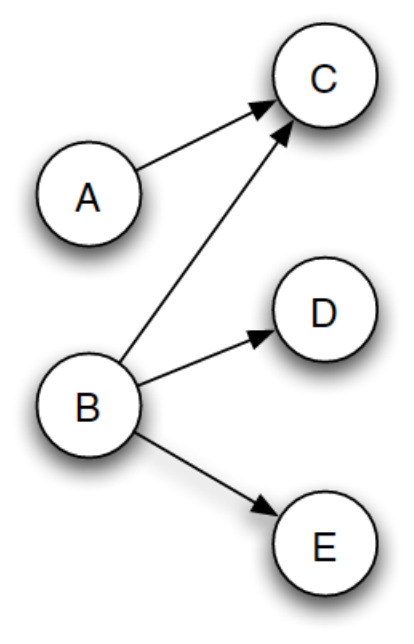
\includegraphics[scale=0.4]{figs/auth-hub.png}
	\caption{graphe de page web}
	\label{fig:auth}
\end{figure}

    \subsubsection*{Algorithme de normalisation}
    
    \begin{itemize}
        \item \textbf{Init} :  $ \forall x \: auth(x) = hub(x) = 1 $
        \item \textbf{Steps}: \\
            $\forall x \: auth(x) = \sum_{y \in hub(x)} hub(y)  $ \\
            $\forall x \: hub(x) = \sum_{y \in auth(x)} auth(y)  $
        \item \textbf{Normalisation} : \\
            $ \forall x \: auth(x) = \frac{auth(x)}{\sum auth} $ \\
            $ \forall x \: hub(x) = \frac{hub(x)}{\sum hub} $
    \end{itemize}

    \subsubsection*{Solution}
    \begin{itemize}
        \item \textbf{Auth} : authorité : liens entrants
        \item \textbf{Conc} : concentrateur : liens sortants
    \end{itemize}

    \begin{center}
    	\begin{tabular}{c|ccccc}
    	     & A & B & C & D & E\\ \hline
    	Auth & 1 & 1 & 1 & 1 & 1\\
    	Conc & 1 & 1 & 1 & 1 & 1\\ \hline
    	Auth & 0 & 0 & 2 & 1 & 1\\
    	Conc & 1 & 3 & 0 & 0 & 0\\ \hline
    	Auth & 0 & 0 & 4 & 3 & 3\\
    	Conc & 2 & 4 & 0 & 0 & 0\\ \hline
    	\end{tabular}
    \end{center}
    
    Normalisation :
    \begin{center}
    	\begin{tabular}{c|ccccc}
    	     & A & B & C & D & E\\ \hline
    	Auth & 0 & 0 & 0.4 & 0.3 & 0.3\\
    	Conc & $\frac{1}{3}$ & $\frac{2}{3}$ & 0 & 0 & 0\\ \hline
    	\end{tabular}
    \end{center}
    
    
\subsection*{Exercice 6}
Calculez les valeurs de PageRank pour chaque page dans le graphe présenté à la Figure \ref{fig:pagerank} après deux itérations avec S = 1.


\begin{figure}[ht!]
	\centering
	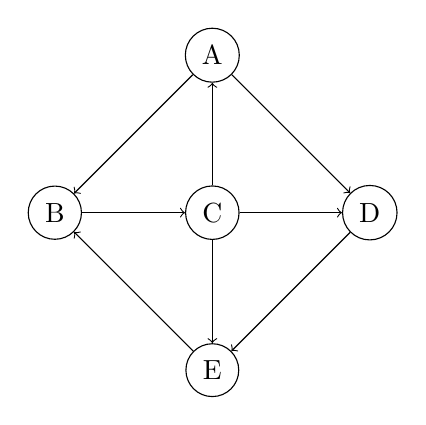
\begin{tikzpicture}[node distance=2cm]
		\tikzstyle{every node}=[draw=black,shape=circle]
		\node (c) at (0,0){C};
		\node[above of=c](a){A};
		\node[below of=c](e){E};
		\node[right of=c](d){D};
		\node[left of=c](b){B};

		\draw[->](a) -- (b);
		\draw[->](a) -- (d);
		\draw[->](b) -- (c);
		\draw[->](c) -- (a);
		\draw[->](c) -- (d);
		\draw[->](c) -- (e);
		\draw[->](d) -- (e);
		%\draw[->](d) -- (c);
		\draw[->](e) -- (b);
	\end{tikzpicture}
	\caption{graphe de page web}
	\label{fig:pagerank}
\end{figure}

    \subsubsection*{Solution}
    Règle de mise à jour : $Pr'(p) = S\ Pr(p) + (1-S) \frac{1}{n} = Pr(p)$.
    Seule la probabilité de suivre un lien à partir d'une page web entre en compte ici.\\
    À chaque itération k, on effectue les mises à jour suivantes :
    \begin{description}
        \item $Pr(A) = \frac{1}{3} Pr(C)$
        \item $Pr(B) = \frac{1}{2} Pr(A) + Pr(E)$
        \item $Pr(C) = Pr(B)$
        \item $Pr(D) = \frac{1}{2} Pr(A) + \frac{1}{3} Pr(C)$
        \item $Pr(E) = \frac{1}{3} Pr(C) + Pr(D)$
    \end{description}
    
    \begin{center}
        \begin{tabular}{c|ccccc}
        k & A & B & C & D & E\\ \hline 
    	0 & $\frac{1}{5}$ & $\frac{1}{5}$ & $\frac{1}{5}$ & $\frac{1}{5}$ & $\frac{1}{5}$\\ \\
    	1 & $\frac{1}{15}$ & $\frac{3}{10}$ & $\frac{1}{5}$ & $\frac{1}{6}$ & $\frac{4}{15}$\\ \\
    	2 & $\frac{1}{15}$ & $\frac{3}{10}$ & $\frac{3}{10}$ & $\frac{1}{10}$ & $\frac{7}{30}$\\
    	\end{tabular}
    \end{center}

\subsection*{Exercice 7}
Dans la Figure \ref{fig:equi}, les nombres à coté des noeuds représentent la valeur de PageRank de la page. Avec ce graphe, les valeurs de PageRank forment-elles un ensemble équilibré? Si oui pourquoi? Si non pourquoi?

\begin{figure}[ht!]
	\centering
	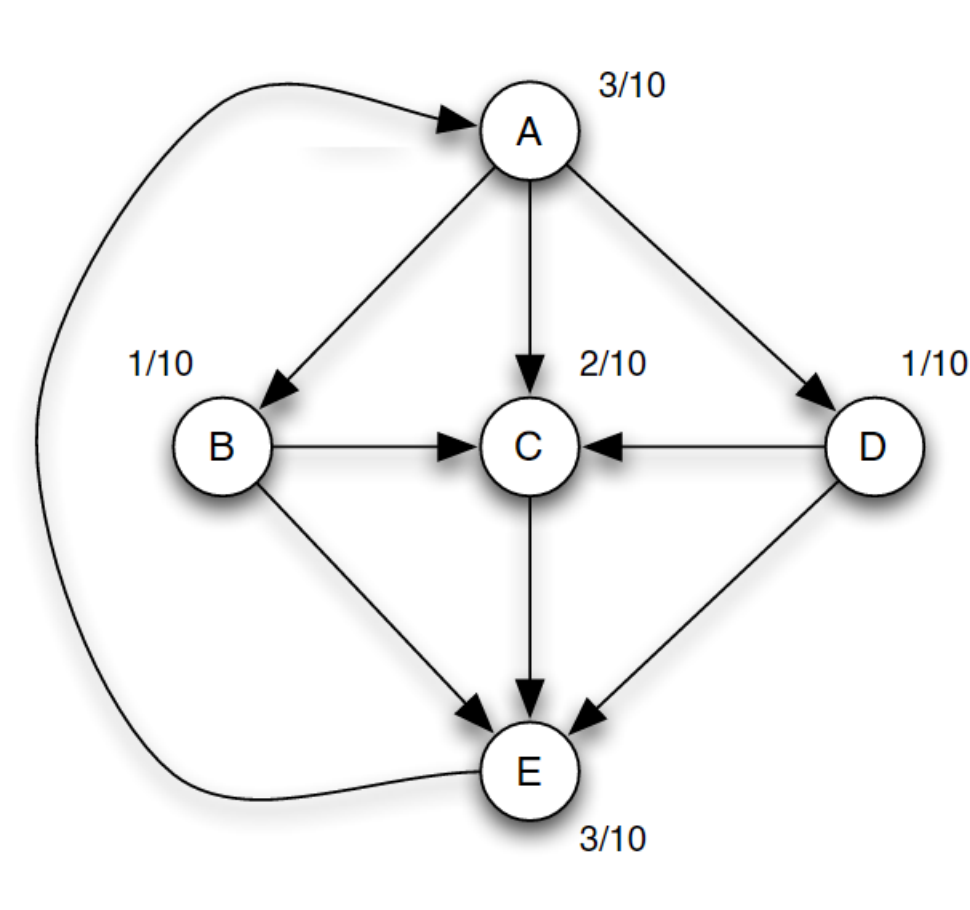
\includegraphics[scale=0.3]{figs/equi.png}
	\caption{graphe de page web}
	\label{fig:equi}
\end{figure}

    \subsubsection*{Solution}
    Il y a deux conditions à respecter pour que les valeurs de PageRank d'un graphe forment un ensemble équilibré :
    \begin{enumerate}
        \item La somme des valeurs doit valoir 1 : $\sum Pr(p_i) = 1$
        \item Une nouvelle itération doit donner les mêmes valeurs : $Pr'(p_i) = Pr(p_i) \ \forall p_i$\\
    \end{enumerate}
    
    Vérifions tout d'abord la première condition :
    $$ \sum Pr(p_i) = \frac{3}{10} + \frac{1}{10} + \frac{2}{10}  + \frac{1}{10}+  \frac{3}{10} = \frac{10}{10} = 1 $$

    Ensuite la seconde :
    \begin{description}
        \item $Pr'(A) = Pr(E) = \frac{3}{10} = Pr(A)$
        \item $Pr'(B) = \frac{1}{3} Pr(A) = \frac{1}{10} = Pr(B)$
        \item $Pr'(C) = \frac{1}{3} Pr(A) + \frac{1}{2} Pr(B) + \frac{1}{2} Pr(D) = \frac{2}{10} = Pr(C)$
        \item $Pr'(D) = \frac{1}{3} Pr(A) = \frac{1}{10} = Pr(D)$
        \item $Pr'(E) = \frac{1}{2} Pr(B) + Pr(C) + \frac{1}{2} Pr(D) = \frac{3}{10} = Pr(E)$\\
    \end{description}

    Nous pouvons donc conclure que nous cet ensemble de valeurs PageRank forme bien un ensemble équilibré.
    

\subsection*{Exercice 8}
		\begin{enumerate}
				\item Calculez les valeurs de PageRank pour chaque page dans le graphe présenté à la Figure \ref{fig:blackhole} après trois itérations avec S = 1.
				\item Que remarquez-vous? Selon vous comment vont évoluer les valeurs
						de PageRank pour un nombre d'itérations de plus en plus grand
				\item Calculez à nouveau les valeurs de PageRank pour chaque page mais pour 2 itérations avec S = 0.5.
		\end{enumerate}
		
    \begin{figure}[ht!]
	\centering
	
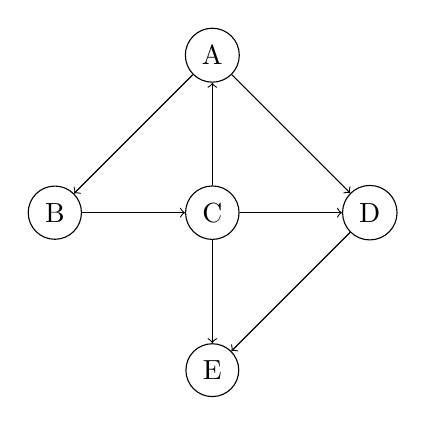
\begin{tikzpicture}[node distance=2cm]
	\tikzstyle{every node}=[draw=black,shape=circle]
	\node (c) at (0,0){C};
	\node[above of=c](a){A};
	\node[below of=c](e){E};
	\node[right of=c](d){D};
	\node[left of=c](b){B};

	\draw[->](a) -- (b);
	\draw[->](a) -- (d);
	\draw[->](b) -- (c);
	\draw[->](c) -- (a);
	\draw[->](c) -- (d);
	\draw[->](c) -- (e);
	\draw[->](d) -- (e);
	%\draw[->](d) -- (c);
	%\draw[->](e) -- (b);
\end{tikzpicture}
\caption{graphe de page web}
\label{fig:blackhole}
\end{figure}
		
    \subsubsection*{Solution}
    \begin{enumerate}
    
    \item Pour S=1, à chaque itération k, on effectue les mises à jour suivantes :
    \begin{description}
        \item $Pr(A) = \frac{1}{3} Pr(C)$
        \item $Pr(B) = \frac{1}{2} Pr(A)$
        \item $Pr(C) = Pr(B)$
        \item $Pr(D) = \frac{1}{2} Pr(A) + \frac{1}{3} Pr(C)$
        \item $Pr(E) = \frac{1}{3} Pr(C) + Pr(D) + Pr(E)$ \\
        \textit{(On ajoute $Pr(E)$ au calcul de E car c'est un noeud "cul-de-sac". Lors d'une itération, il faut prendre en compte le fait qu'une transition est bloquée au niveau de E et retombera donc vers E.)}
    \end{description}
    
    On obtient le résultat qui suit :
    \begin{center}
        \begin{tabular}{c|ccccc}
        k & A & B & C & D & E\\ \hline 
    	0 & $\frac{6}{30}$ & $\frac{6}{30}$ & $\frac{6}{30}$ & $\frac{6}{30}$ & $\frac{6}{30}$\\ \\
    	1 & $\frac{2}{30}$ & $\frac{3}{30}$ & $\frac{6}{30}$ & $\frac{5}{30}$ & $\frac{14}{30}$\\ \\
    	2 & $\frac{2}{30}$ & $\frac{1}{30}$ & $\frac{3}{30}$ & $\frac{3}{30}$ & $\frac{21}{30}$\\ \\
    	3 & $\frac{1}{30}$ & $\frac{1}{30}$ & $\frac{1}{30}$ & $\frac{2}{30}$ & $\frac{25}{30}$\\
    	\end{tabular}
    \end{center}
    
    \item On remarque qu'il y a une accumulation au niveau du noeud E.
    Sa valeur va tendre vers 1 alors que toutes les autres tendent vers 0.
    
    \item Pour S=0.5, à chaque itération k, on effectue les mises à jour suivantes :
    \begin{description}
        \item $Pr'(A) = \frac{1}{6} Pr(C) + \frac{1}{10}$
        \item $Pr'(B) = \frac{1}{4} Pr(A) + \frac{1}{10}$
        \item $Pr'(C) = \frac{1}{2} Pr(B) + \frac{1}{10}$
        \item $Pr'(D) = \frac{1}{4} Pr(A) + \frac{1}{6} Pr(C) + \frac{1}{10}$
        \item $Pr'(E) = \frac{1}{6} Pr(C) + \frac{1}{2} Pr(D) + \frac{1}{2} Pr(E) + \frac{1}{10}$
    \end{description}
    
    Le tableau résultant est :
    \begin{center}
        \begin{tabular}{c|ccccc}
        k & A & B & C & D & E\\ \hline 
    	0 & $\frac{6}{30}$ & $\frac{6}{30}$ & $\frac{6}{30}$ & $\frac{6}{30}$ & $\frac{6}{30}$\\ \\
    	1 & $\frac{4}{30}$ & $\frac{4.5}{30}$ & $\frac{6}{30}$ & $\frac{5.5}{30}$ & $\frac{10}{30}$\\ \\
    	2 & $\frac{4}{30}$ & $\frac{4}{30}$ & $\frac{5.25}{30}$ & $\frac{5}{30}$ & $\frac{11.75}{30}$\\
    	\end{tabular}
    \end{center}


\end{enumerate}

\end{document}
